\documentclass[a4paper,10pt,english]{article}
%\documentclass[12pt,preprint]{aastex}
\usepackage[utf8]{inputenc}
\usepackage[margin=0.5in]{geometry} % narrow margins

% Document formatting
\setlength{\parindent}{0mm}
\setlength{\parskip}{1.5mm}

\usepackage{amsfonts}
\usepackage{graphicx}
\usepackage{float}
\usepackage{cite}
\usepackage{amsmath}
\usepackage{epsfig,floatflt}
\usepackage{hyperref}
\usepackage{listings}
\usepackage[table,xcdraw]{xcolor}
\usepackage{booktabs}
\usepackage{subfig}
\usepackage{algpseudocode}
\usepackage{algorithm}
%\usepackage{amsmath,graphicx,varioref,verbatim,amsfonts,geometry,amssymb,dsfont,blindtext}
\hypersetup{colorlinks=true}
\usepackage{xcolor}
\usepackage{hhline}
\usepackage[export]{adjustbox}
\definecolor{LightGray}{gray}{0.95}
\definecolor{dkgreen}{rgb}{0,0.6,0}
\definecolor{gray}{rgb}{0.5,0.5,0.5}
\definecolor{mauve}{rgb}{0.58,0,0.82}
\definecolor{mygray}{rgb}{0.9,0.9,0.9}
\definecolor{LightGray}{gray}{0.95}
\lstset{frame=tb,
	language=Python,
	aboveskip=3mm,
	belowskip=3mm,
	showstringspaces=false,
	columns=flexible,
	basicstyle={\small\ttfamily},
	numbers=none,
	numberstyle=\tiny\color{gray},
	keywordstyle=\color{blue},
	commentstyle=\color{dkgreen},
	stringstyle=\color{mauve},
	backgroundcolor=\color{mygray},
	breaklines=true,
	postbreak=\mbox{\textcolor{red}{$\hookrightarrow$}\space}
	%breakatwhitespace=true,
	%tabsize=3
}

%\usepackage[english]{babel}
%\usepackage{fancyhdr}
%\usepackage{lastpage}
%
%\pagestyle{fancy}
%\fancyhf{}
%
%\rfoot{Page \thepage \hspace{1pt} of \pageref{LastPage}}
\pagenumbering{arabic}

\begin{document}
\title{FYS-STK4155 Project 1}
\author{Bendik Steinsvåg Dalen \& Gabriel Sigurd Cabrera}
%\maketitle

\twocolumn[
\maketitle
\begin{abstract}
	dtcfvgbjhkgvfcdxszeasxrdtgyubhnijhugfvcdfguhij ftufykubhk nj jkdsi jkjk dsjknslj fd,nøj ka n,sdf jknm bnjdsajk nmnj mbfdjksa ,nfdsa mn n,asdf\\\\
\end{abstract}
]

%\begin{@twocolumnfalse}
%%	\maketitle
%	\begin{abstract}
%		dtcfvgbjhkgvfcdxszeasxrdtgyubhnijhugfvcdfguhij ftufykubhk nj jkdsi jkjk dsjknslj fd,nøj ka n,sdf jknm bnjdsajk nmnj mbfdjksa ,nfdsa mn n,asdf
%	\end{abstract}
%\end{@twocolumnfalse}

\section*{Introduction}
\label{sec:introduction}

The purpose of this report is to analyze the performance of several regression methods – Ordinary Least Squares (OLS), Ridge Regression, and \textsc{lasso}\footnote{Short for \textit{least absolute shrinkage and selection operator}.} Regression.  In addition to implementing these regression methods, we will be validating (and cross-validating) our results by calculating the \textit{mean squared error}, \textit{bias}, and \textit{variance}, giving us an understanding of how these models' predictive capabilities vary as functions of complexity.

Once we have a clear picture of how these regression models behave, we hope to determine which model best fits our input data.  This will require analyzing our validation data and determining what complexity and hyperparameter minimizes our total error.

To actually implement all of this, we will use \texttt{python} and create a \texttt{class Regression}, initialized with a set of inputs $\mathbf{X} \in \mathbb{R}^{n \times p}$ and $\mathbf{y} \in \mathbb{R}^n$.  Once an instance of the object is created, methods such as \texttt{Regression.poly(degree, alpha)} or \texttt{Regression.\textsc{lasso}(degree, alpha)} can be called in order to perform OLS/Ridge regression or \textsc{lasso} regression, respectively.  Other methods, such as \texttt{Regression.mse()} will give us our \textit{mean squared error}.

We will be using two datasets – the first will be generated by the sum of the \textit{Franke function} and some normally distributed noise, and the second will consist of real data taken from the \textit{U.S. Geological Survey}.

%Things we need to write about:
%
%Background on regression analysis and resampling methods.
%Mention:
%	OLS
%	Ridge
%	\textsc{lasso}
%	k-fold cross-validation
%	Bias-Variance trade of?
%
%We will first study how they preform for the two dimensional Franke function. (A bit about the Franke function, maybe a tldr for the method).
%
%We will then implement them for some real terrain data for Møsvatn Austfjell in Norway. mm. (biggest lake in Norway ) %\cite{https://no.wikipedia.org/wiki/Møsvatn}


%Discuss background, physical importance and possibly some history of
%the problem that is being studied in this paper.

\section*{Data}
\label{sec:data}

\subsection*{The Franke Function}

The first dataset will be given by the \textit{Franke function}, which is defined as follows:

\begin{align*}
f(x,y) &= \frac{3}{4} \exp \left( -\frac{(9x-2)^2}{4} -\frac{(9y-2)^2}{4} \right) \\ &+ \frac{3}{4} \exp \left( -\frac{9x+1}{49} -\frac{9y+1}{10} \right) \\ &+ \frac{1}{2} \exp \left( -\frac{(9x-7)^2}{4} -\frac{(9y-3)^2}{4} \right) \\ &- \frac{1}{5} \exp \left( -(9x-4)^2 - (9y-7)^2 \right)
\end{align*}

We will be solving the Franke function for 100 $x$-values and 100 $y$-values in the range $[0,1]$, leaving us with a grid containing a total of 10000 $xy$ coordinate pairs.  This leaves us with the values plotted in Figure \ref{fig_Franke}.

\begin{figure}[H]
	\centering
	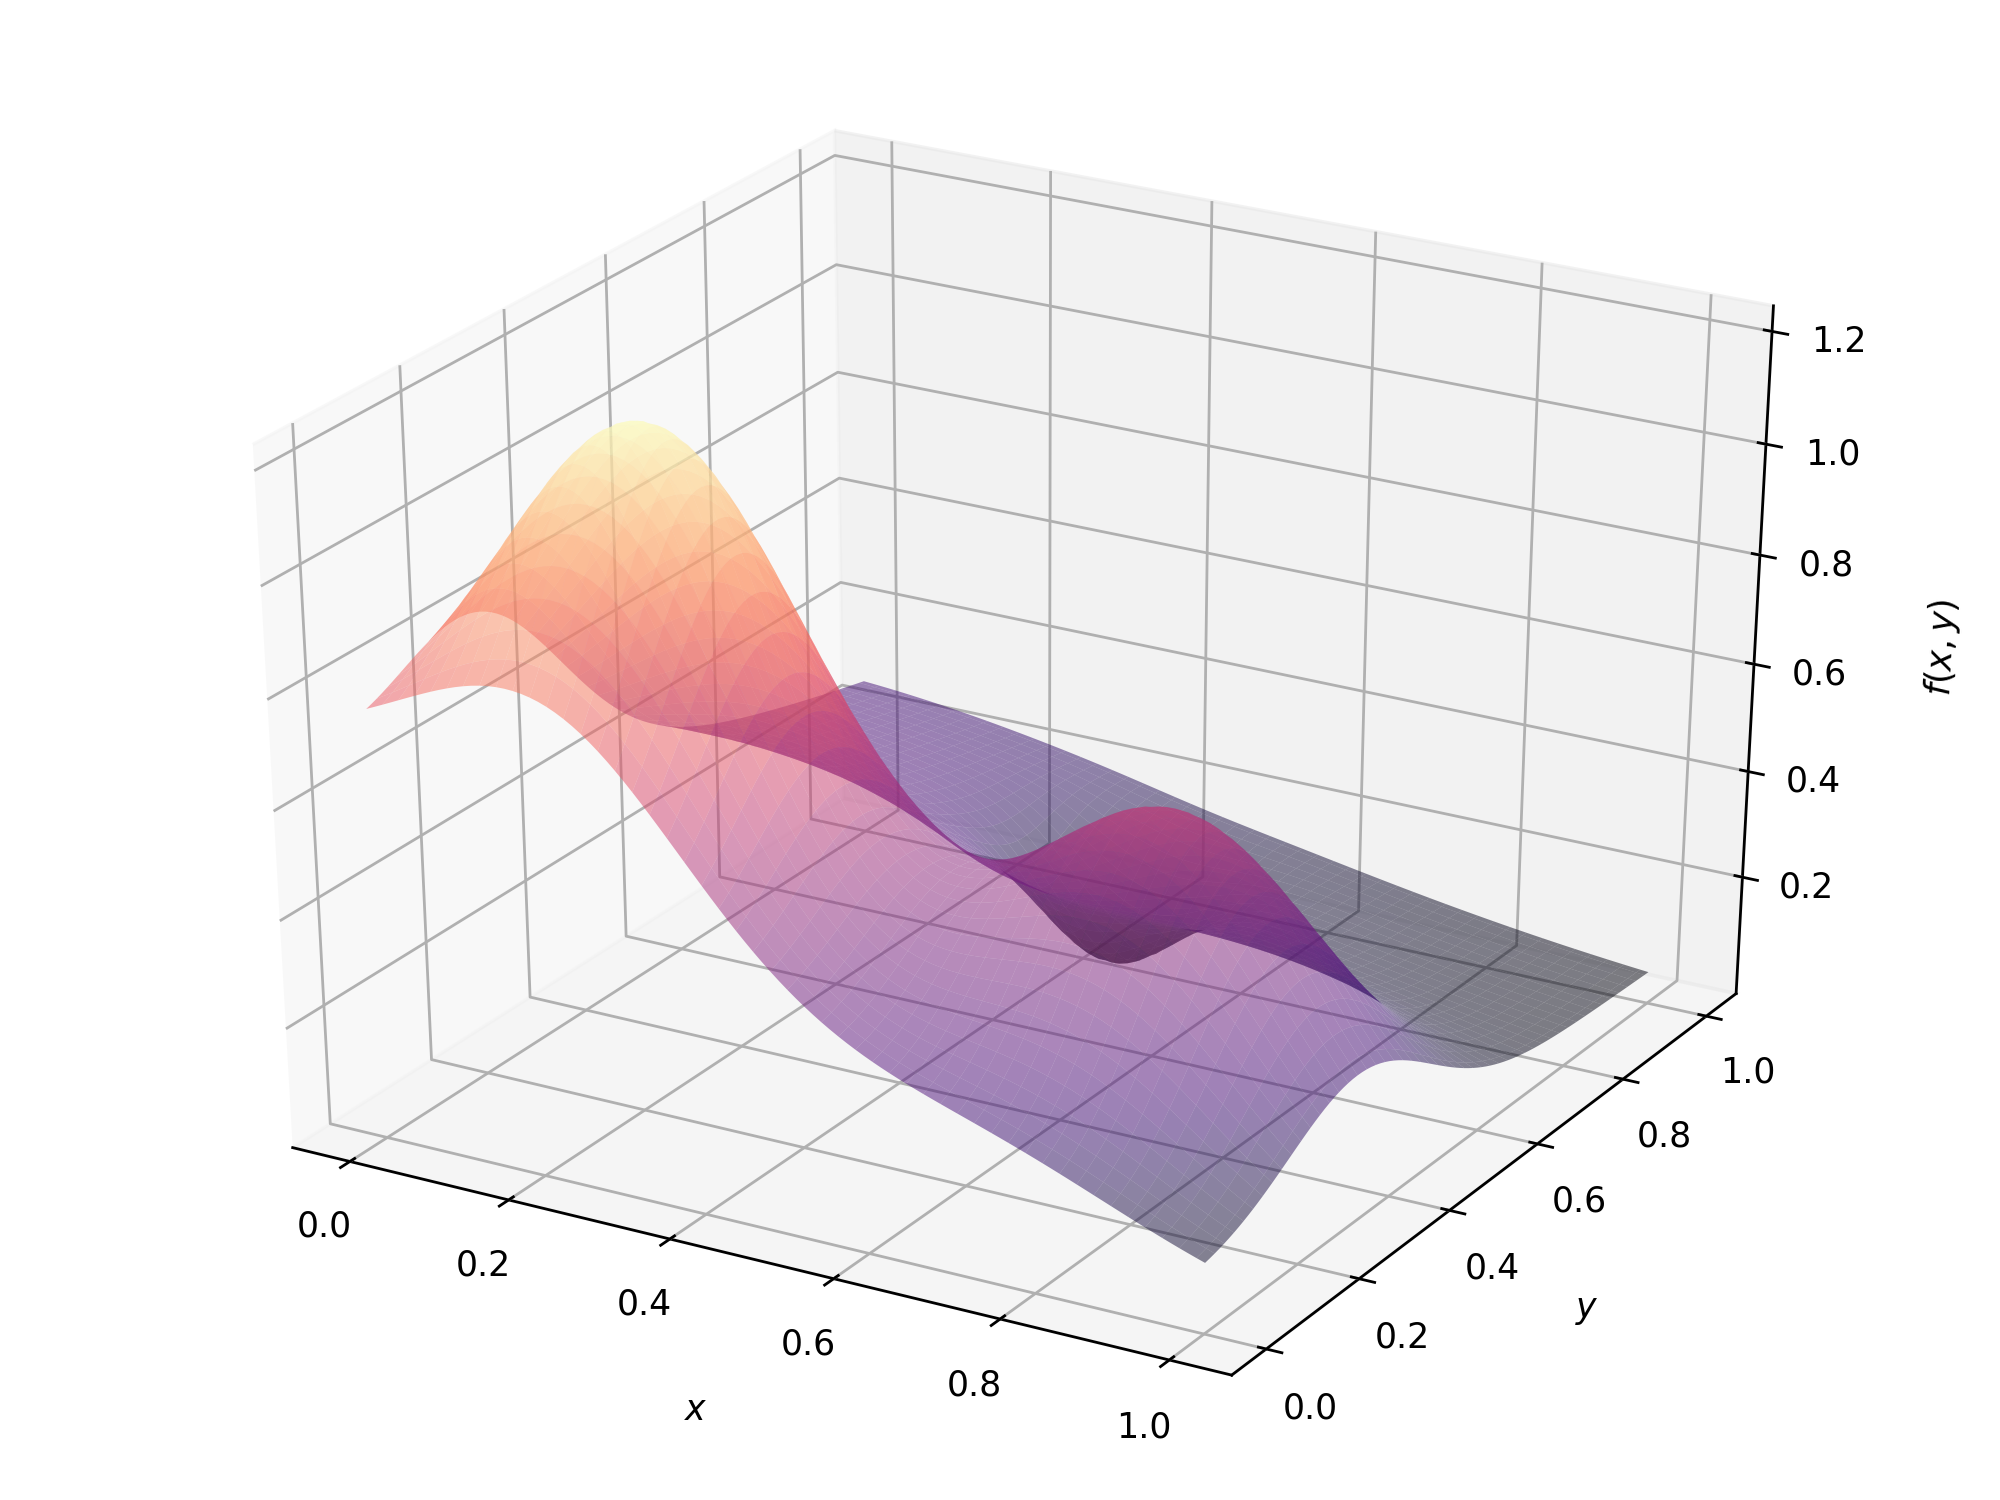
\includegraphics[width = 0.5\textwidth, center]{../franke_output/Franke.png}
	\caption{The \textit{Franke function} for $x$ and $y$ values ranging from zero to one. \label{fig_Franke}}
\end{figure}

In addition, we will also be adding \textit{Gaussian noise} to each value $f(x,y)$, such that we are left with values as seen in Figure \ref{fig_Franke_noise}.

\begin{figure}[H]
	\centering
	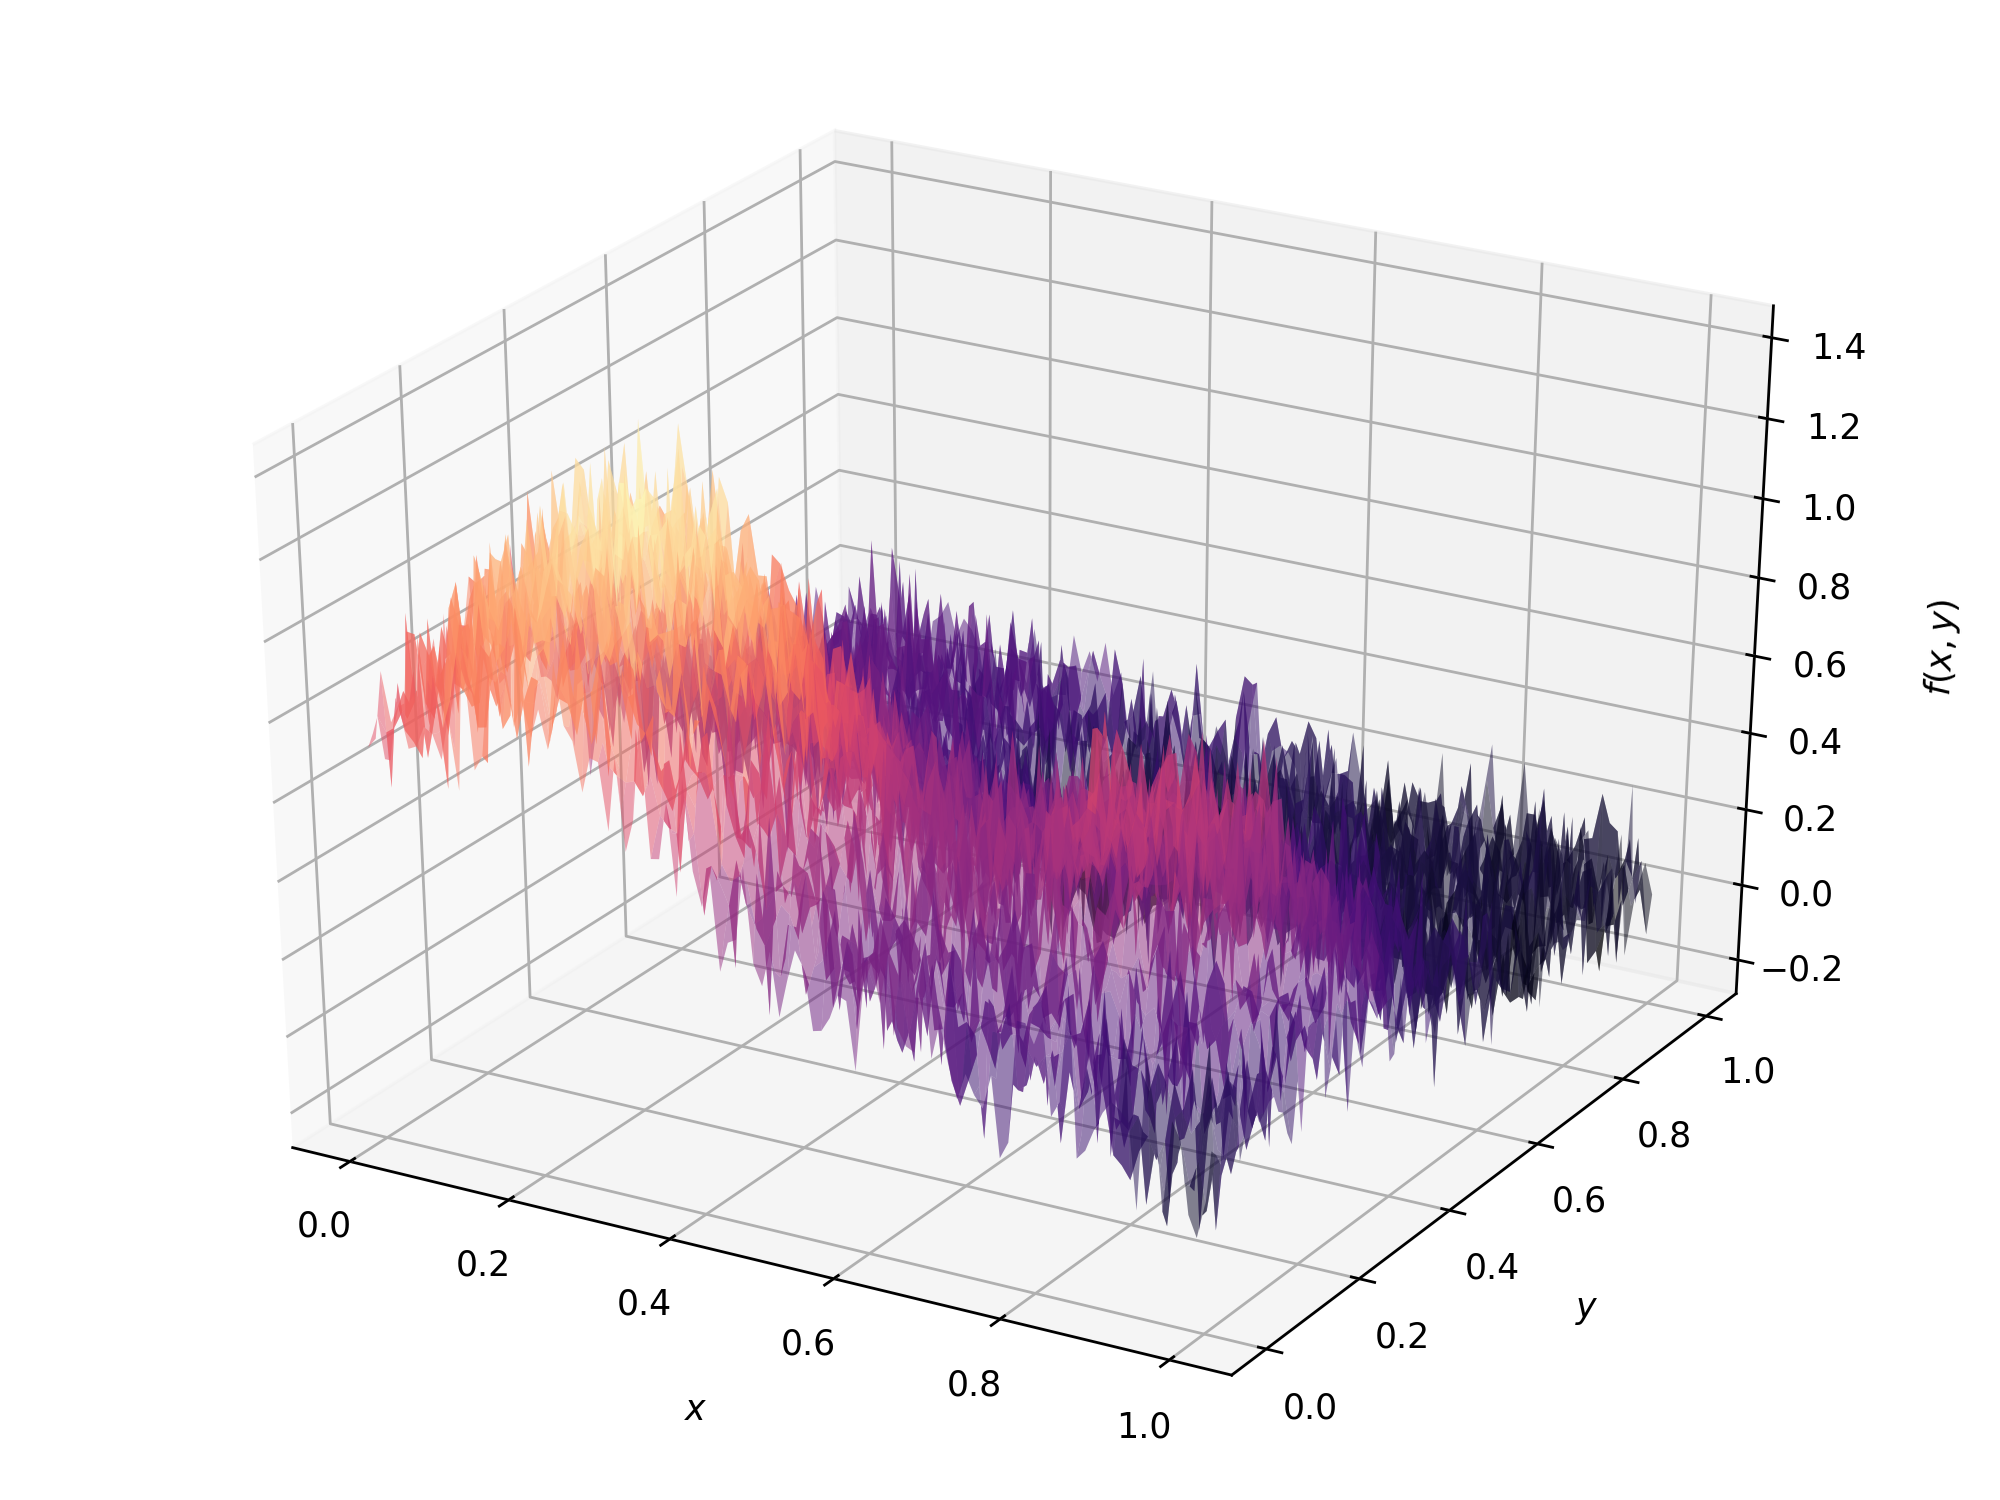
\includegraphics[width = 0.5\textwidth, center]{../franke_output/Franke_noise.png}
	\caption{The \textit{Franke function} for $x$ and $y$ values ranging from zero to one, with a Gaussian noise $N(0,0.01)$\label{fig_Franke_noise}}
\end{figure}

\subsection*{Møsvatn Austfjell}

For our second dataset, we will be using real data taken from the \textit{U.S. Geological Survey} \cite{earthexplorer} official website \url{https://earthexplorer.usgs.gov/}.  More specifically, we will be using a \texttt{.tif} file containing altitude data for a rectangular region of Møsvatn Austfjell shown in Figure \ref{fig_austfjell}.

\begin{figure}[H]
	\centering
	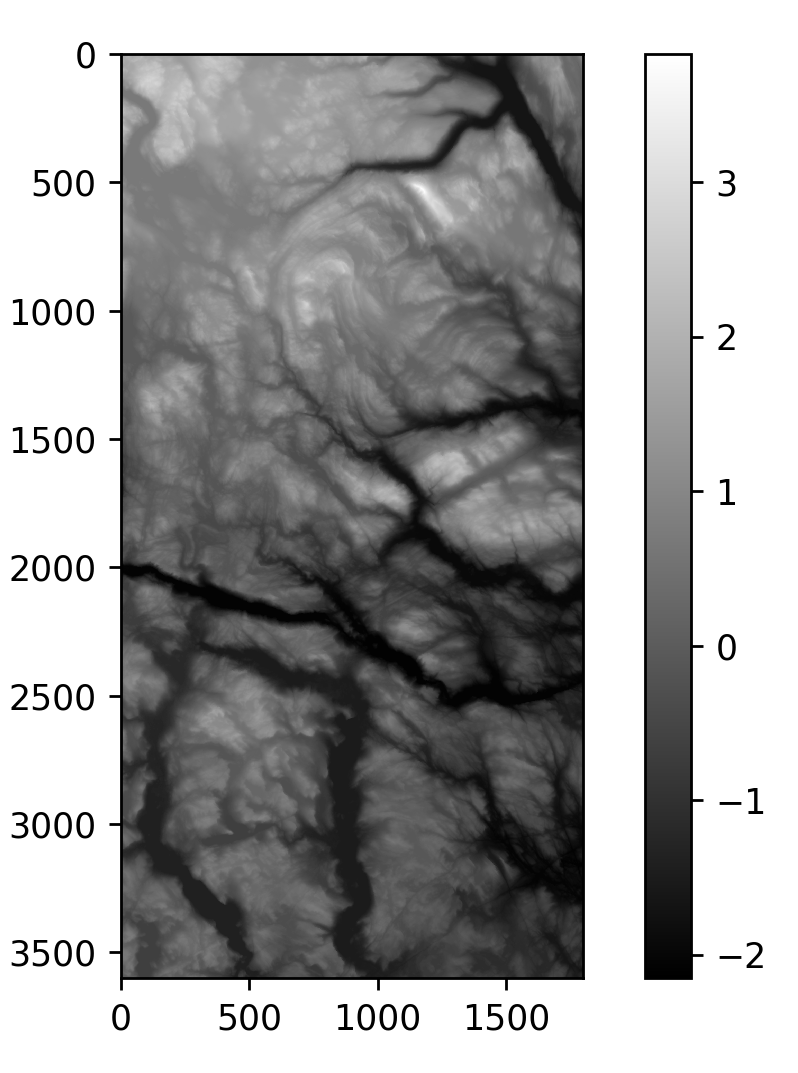
\includegraphics[width = 0.4\textwidth, center]{real_data.png}
	\caption{Altitude data from Møsvatn Austfjell, from the USGS website \cite{earthexplorer}.\label{fig_austfjell}}
\end{figure}	

\section*{Method}

\subsection*{Generalization of Multidimensional Polynomials}

If we wish to construct a $p$-dimensional polynomial of degree $d$, we need to know what terms need to be included to give us a completely generalized polynomial.  For a 1-D polynomial of second degree, we would have three terms:

\begin{equation*}
f(x) = \beta_1 + \beta_2 x + \beta_3 x^2
\end{equation*}

Where $\beta$ is a vector containing each coefficient.	For a 2-D polynomial of second degree, we would have 6 terms:

\begin{equation*}
f(x,y) = \beta_1 + \beta_2 x + \beta_3 y + \beta_4 xy + \beta_5 x^2 + \beta_6 y^2
\end{equation*}

And for a 3-D polynomial of second degree, we would have 10 terms:

\begin{align*}
f(x,y,z) &= \beta_1 + \beta_2 x + \beta_3 y + \beta_4 z + \beta_5 xy \\ &+ \beta_6 xz + \beta_7 yz + \beta_8 x^2 + \beta_9 y^2 + \beta_{10} z^2
\end{align*}

There are many possible combinations of $p$ and $d$, and the number of terms blows up significantly as these values increase.  We can, however, create a general expression \cite{2482654} for any $p$ and $d$ using summation notation:

\begin{equation}
\label{eq_method_0}
f(\mathbf{x}) = \sum_{\sum_{j = 1}^d i_j \leq p} \left( \beta_{i_1, i_2, \cdots, i_d} \prod_{k = 1}^d x_k^{i_k} \right)
\end{equation}

Alternatively, a simple \texttt{python} script can be used to find all the terms' exponents by calculating all permutations of the natural numbers from zero to $d$ in sets of length $p$, then removing all results whose sum is greater than $d$.

\begin{lstlisting}[showstringspaces=false,language=Python,firstnumber = 1]
powers = np.arange(0, degree + 1, 1)
powers = np.repeat(powers, p)
exponents = list(permutations(powers, p))
exponents = np.unique(exponents, axis = 0)

if p != 1:
expo_sum = np.sum(exponents, axis = 1)
valid_idx = np.where(np.less_equal(expo_sum, degree))[0]
exponents = np.array(exponents, dtype = np.int64)
exponents = exponents[valid_idx]
else:
exponents = np.array(exponents, dtype = np.int64)
\end{lstlisting}


\subsection*{Ordinary Least-Squares (OLS) Regression}

We are given a $p+1$-dimensional dataset\footnote{Meaning a set of $p$ input features and 1 output.} consisting of $N$ datapoints per feature such that:

\begin{equation}
\label{eq_method_1}
\mathbf{X} = \begin{bmatrix} X_{1,1} & X_{1,2} & \cdots & X_{1,p} \\ X_{2,1} & X_{2,2} & \cdots & X_{2,p} \\ \vdots & \vdots & \ddots & \vdots \\ X_{N,1} & X_{N,2} & \cdots & X_{N,p} \end{bmatrix} \qquad \mathbf{y} = \begin{bmatrix} y_1 \\ y_2 \\ \vdots \\ y_N \end{bmatrix}
\end{equation}

Where the $N \times p$ matrix $\mathbf{X}$ contains the dataset's \textit{input data}, and the $N$-vector $\mathbf{y}$ contains its \textit{output data}, such that each row in $\mathbf{X}$ corresponds to a single output in $\mathbf{y}$.

Now, we wish to find a $p$-dimensional polynomial of degree $d$ which most closely matches our dataset. We will need a design matrix $\mathbf{A}$; this will require using the knowledge presented in (\ref{eq_method_0}), since a design matrix should contain each polynomial term as an individual column.

Next, we will be using the method of \textit{least squares} \cite{hastie_tibshirani_friedman_2013}, whereby we attempt to minimize the \textit{residual sum of squares}:

\begin{equation*}
RSS(\beta) = \sum_{i=1}^N (y_i - \mathbf{A}_i^\textsc{t} \beta)^2 
\end{equation*}

Where $\mathbf{A}_i$ represents the $i$\textsuperscript{th} row in $\mathbf{A}$, and $beta$ is the set of coefficents in the aforementioned polynomial; in matrix form, this can be written more concisely:

\begin{equation*}
RSS(\beta) = (\mathbf{y} - \mathbf{A} \beta)^\textsc{t}(\mathbf{y} - \mathbf{A} \beta)
\end{equation*}

To minimize the $RSS$, we can differentiate it with respect to $\beta$ and set the right-hand side equal to zero – this allows us to solve for $\beta$, which will give us the coefficients to the polynomial that best matches our dataset:

\begin{equation*}
\mathbf{A}^\textsc{t} (\mathbf{y} - \mathbf{A} \beta) = 0 \iff \mathbf{A}^\textsc{t} y = \mathbf{A}^\textsc{t} \mathbf{A} \beta
\end{equation*}

Solving for $\beta$ then gives us our desired result:

\begin{equation}
\label{eq_method_2}
\beta = (\mathbf{A}^\textsc{t} \mathbf{A} ) ^{-1} \mathbf{A}^\textsc{t} \mathbf{y}
\end{equation}

Using the set of coefficients given by (\ref{eq_method_2}), we can then match the dataset from (\ref{eq_method_1}) as effectively as possible.

\subsection*{Ridge Regression}

The solution for $\beta$ given in (\ref{eq_method_2}) can be used without issue in many cases, but if the matrix $\mathbf{A}$ is singular\footnote{Meaning that $\text{det}(\mathbf{A}) = 0$}, we run into an issue – namely, we cannot take the inverse of a singular matrix!  As a result, we must look to more robust methods; one such method is called \textit{ridge regression}.  

The process of obtaining our vector of coefficients $\beta$ via ridge regression is functionally very similar to that of OLS.  The main difference is that we include an extra term in the residual sum of squares:

\begin{equation*}
RSS(\beta) = \sum_{i=1}^N (y_i - \mathbf{A}_i^\textsc{t} \beta)^2 + \lambda \sum_{i=1}^N \beta^2
\end{equation*}

In matrix form, this can be rewritten:	

\begin{equation*}
RSS(\beta) = (\mathbf{y} - \mathbf{A} \beta)^\textsc{t}(\mathbf{y} - \mathbf{A} \beta) + \lambda \beta^\textsc{t} \beta
\end{equation*}

Where $\lambda$, known as the \textit{hyperparameter}, is a scalar value. Performing the same process as in the previous subsection, we are left with a solution similar to that in (\ref{eq_method_2}):

\begin{equation}
\label{eq_method_3}
\beta = (\mathbf{A}^\textsc{t} \mathbf{A} + \lambda \mathbf{I}) ^{-1} \mathbf{A}^\textsc{t} \mathbf{y}
\end{equation}

In cases where $\mathbf{A}$ is singular, it is therefore possible to make very few changes to the OLS algorithm and still get a good result, one must simply optimize the hyperparameter and find a $\lambda$ that minimizes the \textit{mean squared error} (yet to be introduced) of our polynomial approximation.

\subsection*{\textsc{lasso} Regression}

\begin{algorithm}[H]
	\caption{The \textsc{lasso} algorithm, over the course of $500$ iterations.}
	\begin{algorithmic}[1]
		\State $z = \sum_i A_i^2$
		\State $i = 0$
		\While{$i \leq 500$}
		\State $i = i + 1$
		\State $j = 0$
		\While{j < p}
		\State $\hat{y} = \sum_{k \neq j} \beta A_{*,k}$
		\State $\rho = \sum_k A_{*,k} (\mathbf{y} - \mathbf{\hat{y}})$
		\If {$\rho < -\lambda/2$}
		\State $\beta_j = (\rho + \lambda/2)/z_j$
		\ElsIf {$\rho > \lambda/2$}
		\State $\beta_j = (\rho - \lambda/2)/z_j$
		\Else
		\State $\beta_j = 0$
		\EndIf
		\EndWhile		
		\EndWhile
	\end{algorithmic}
\end{algorithm}


The \textit{least absolute shrinkage and selection operator}, commonly abbreviated as \textit{\textsc{lasso}}, is a method that implements the \textbf{L1} norm in place of the \textbf{L2} (or Euclidian) norm used in ridge regression.  The residual sum of squares is therefore given by:

\begin{equation}
\label{eq_method_4}
RSS(\beta) = \sum_{i=1}^N (y_i - \mathbf{A}_i^\textsc{t} \beta)^2 + \lambda \sum_{i=1}^N |\beta|
\end{equation}

Unfortunately, differentiating the above with respect to $\beta$ will not work as intended, since we cannot take the matrix-form derivative of $\lambda \sum_{i=1}^N |\beta|$.  As a result, we must use an iterative \textit{gradient descent} method to minimize the right-hand side of (\ref{eq_method_4}).

\subsection*{Mean Squared Error}

To get a measure of success with respect to the implemented method and parameters, we can calculate the mean difference in the squares of each measured output $y_i$ and their respective predicted outputs $\hat{y}_i$:

\begin{equation}
MSE(\mathbf{y}, \mathbf{\hat{y}}) = \frac{1}{N} \sum_{i=1}^{N} (y_i - \hat{y}_i)^2 = \mathbb{E}\left[(\mathbf{y}-\hat{\mathbf{y}})^{2}\right]
\end{equation}

The lower the $MSE$, the closer the polynomial approximation is to the original dataset.  If it is too low, however, we run the risk of overfitting our dataset, which is not desireable either – fortunately, this not an issue within the scope of this report.

\subsection*{R\textsuperscript{2} Score}

Another measure of success is the \textit{coefficient of determination}, colloquially known as the $R^2$ score, is given by the following expression:

\begin{equation}
R^2 = 1 - \frac{\sum_{i=1}^N (y_i - \hat{y}_i)^2 }{\sum_{i=1}^N (y_i - \bar{y}_i)^2 }
\end{equation}

The closer $R^2$ is to one, the closer the polynomial approximation is to the input/output dataset, although a perfect score can once again arise due to overfitting just as in the case of the $MSE$.

\subsection*{Bias-Variance Tradeoff}

Before we continue, we can decompose the range of outputs $\mathbf{y}$ as follows:

\begin{equation}
\label{eq_method_5}
\mathbf{y}(\mathbf{X}) = f(\mathbf{X}) + N(0, \sigma) 
\end{equation}

Where $f(\mathbf{X})$ represents the \textit{actual} function used to generate the dataset, and $N(0,\sigma)$ is a Gaussian noise with a standard deviation of $\sigma$.

As a regression model increases in complexity\footnote{For a polynomial regression, this would refer to its \textit{degree}.}, it so happens that the \textit{variance} of a prediction increases.  Variance is defined as follows:

\begin{equation}
\label{eq_method_6}
\text{Var}(\mathbf{y}) = \frac{1}{n} \sum_{i=1}^{n} (y_i - \mathbb{E}[\mathbf{y}] )
\end{equation}

On the other hand, we have that the \textit{bias} of the prediction decreases as the complexity increases.  We define the bias as:

\begin{equation}
\label{eq_method_7}
\text{Bias}(\mathbf{y}) = \frac{1}{n} \sum_{i=1}^{n} (f_i - \mathbb{E}[\mathbf{y}] )
\end{equation}

Note that in order to calculate the bias, we need to know the original function $f$ used to generate $\mathbf{y}$.

Interestingly enough, taking the sum of (\ref{eq_method_6}) and (\ref{eq_method_7}) as well as $\sigma^2$ will yield the \textit{mean squared error}.  We will show this to be the case in the following subsection.

\subsubsection*{Derivation}

We wish to show that:
\begin{equation}
\label{eq_method_8}
\mathbb{E}\left[(\mathbf{y}-\hat{\mathbf{y}})^{2}\right]
=\frac{1}{n} \sum_{i=1}^{n}(f_{i}-\mathbb{E}[\hat{\mathbf{y}}])^{2}+\frac{1}{n} \sum_{i=1}^{n}(\hat{y}_{i}-\mathbb{E}[\hat{\mathbf{y}}])^{2}+\sigma^{2}
\end{equation}

We begin by rewriting the $MSE$ into summation notation, decomposing the terms as defined in (\ref{eq_method_5}), and adding/subtracting a term $\mathbb{E}[\hat{\mathbf{y}}]$:

\begin{align*}
\mathbb{E}\left[(\mathbf{y}-\hat{\mathbf{y}})^{2}\right] &= \frac{1}{n} \sum_{i=1}^{n} ( y_i - \hat{y}_i )^2 = \frac{1}{n} \sum_{i=1}^{n} ( f_i + \varepsilon - \hat{y}_i )^2 \\
&= \frac{1}{n} \sum_{i=1}^{n} ( f_i + \varepsilon - \hat{y}_i  + \mathbb{E}[\hat{\mathbf{y}}] - \mathbb{E}[\hat{\mathbf{y}}] )^2
\end{align*}

Next, we set $a \equiv f_i - \mathbb{E}[\hat{\mathbf{y}}] $ and $b \equiv \hat{y}_i - \mathbb{E}[\hat{\mathbf{y}}]$ and expand:

\begin{equation*}
\frac{1}{n} \sum_{i=1}^{n} (a - b + \varepsilon )^2
= \frac{1}{n} \sum_{i=1}^{n} ( a^2 - 2ab + b^2 - 2b\varepsilon + \varepsilon^2 + 2a\varepsilon )
\end{equation*}

The next few steps are messy, and require lots of algebraic manipulation:	

\begin{align*}	
&= \frac{1}{n} \sum_{i=1}^{n} ( f_i - \mathbb{E}[\hat{\mathbf{y}}] )^2 
+ \frac{1}{n} \sum_{i=1}^{n} ( \varepsilon^2 )
+ \frac{1}{n} \sum_{i=1}^{n} ( \hat{y}_i - \mathbb{E}[\hat{\mathbf{y}}] )^2 
\\&- \frac{2}{n} \sum_{i=1}^{n} \varepsilon ( \hat{y}_i - \mathbb{E}[\hat{\mathbf{y}}] )
+ \frac{2}{n} \sum_{i=1}^{n} \varepsilon ( f_i - \mathbb{E}[\hat{\mathbf{y}}] )
\\&- \frac{2}{n} \sum_{i=1}^{n} ( f_i - \mathbb{E}[\hat{\mathbf{y}}] ) ( \hat{y}_i - \mathbb{E}[\hat{\mathbf{y}}] )
= \frac{1}{n} \sum_{i=1}^{n} ( f_i - \mathbb{E}[\hat{\mathbf{y}}] )^2 
\\&+ \frac{1}{n} \sum_{i=1}^{n} ( \hat{y}_i - \mathbb{E}[\hat{\mathbf{y}}] )^2 
+ \sigma^2
- \mathbb{E}[\varepsilon] \frac{2}{n} \sum_{i=1}^{n} ( \hat{y}_i - \mathbb{E}[\hat{\mathbf{y}}] )
\\&+ \mathbb{E}[\varepsilon] \frac{2}{n} \sum_{i=1}^{n} ( f_i - \mathbb{E}[\hat{\mathbf{y}}] )
-\frac{2}{n} \sum_{i=1}^{n} ( f_i - \mathbb{E}[\hat{\mathbf{y}}] ) ( \hat{y}_i - \mathbb{E}[\hat{\mathbf{y}}] )
\end{align*}

Finally, we see that our original assumption given by (\ref{eq_method_8}) is correct.

\begin{equation*}
= \frac{1}{n} \sum_{i=1}^{n} ( f_i - \mathbb{E}[\hat{\mathbf{y}}] )^2 
+ \frac{1}{n} \sum_{i=1}^{n} ( \hat{y}_i - \mathbb{E}[\hat{\mathbf{y}}] )^2 
+ \sigma^2 \qquad \square
\end{equation*}

Where $\frac{1}{n} \sum_{i=1}^{n} ( f_i - \mathbb{E}[\hat{\mathbf{y}}] )$ is the \textit{bias} and
$\frac{1}{n} \sum_{i=1}^{n} ( \hat{y}_i - \mathbb{E}[\hat{\mathbf{y}}] )^2$ is the \textit{variance}.	

\subsection*{Cross-Validation}

So far, all our methods involving validation\footnote{This refers to calculating the $MSE$, variance, bias, and so on.} may have involved the separation of our data into a training and testing set, whereby the vector of coefficients is calculated using the \textit{training} set, and the validation is performed on the \textit{testing} set that remains.	There is however one more way to obtain a clearer picture of how well a model works: \textit{k-fold} cross validation.	

In short, once the training and testing set have been separated, we can choose a value for $k$.  Next, we divide the training set into $k$ equally sized parts\footnote{We can have slightly unequal-sized parts without it being an issue, if the size of the dataset doesn't divide perfectly into $k$.}.  The next step is to be performed $k$ times; here we take $k-1$ of the parts and combine them into a temporary training set, and leave the last part as our testing set, and we perform validation on the testing set, and save the values.  During each iteration, we must shuffle our parts such that each step has a unique training-testing split.

Finally, we can take all the calculated $MSE$ values, among others, and take their average.  This leaves us with a well-rounded result \textit{without} the need for more input data!

\section*{Results}
\label{sec:results}

Using our \texttt{class Regression}, we implemented each aforementioned regression methods; using cross-validation, we tested for a variety of conditions so as to optimize our potential models. 

\subsection*{The Franke Function}

\begin{figure}[H]
	\centering  
	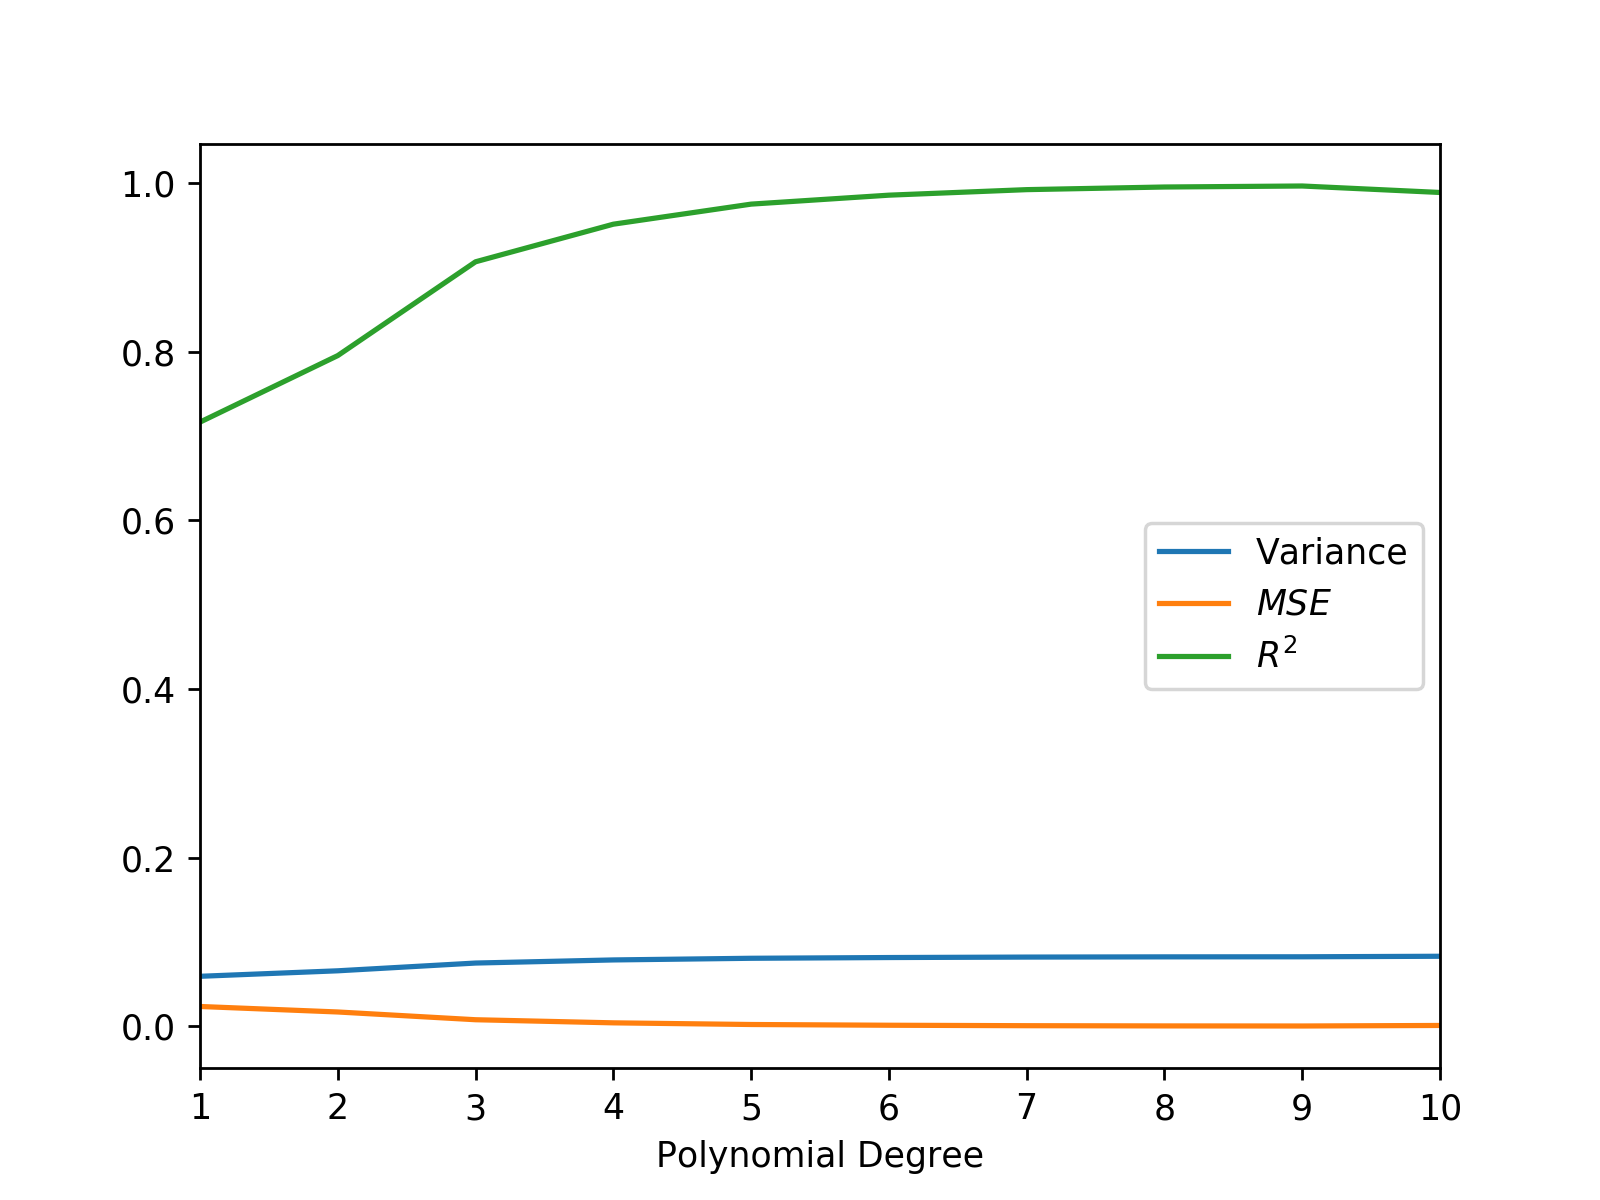
\includegraphics[width = 0.5\textwidth, center]{../franke_output/part_A.png}
	\caption{The $MSE$, the $R^2$-score, and the variance $\sigma$ in the vector of coefficients $\beta$, as functions of the polynomial degree after performing OLS on the Franke function}
	\label{fig_4}
\end{figure}

\begin{figure}[H]
	\centering 
	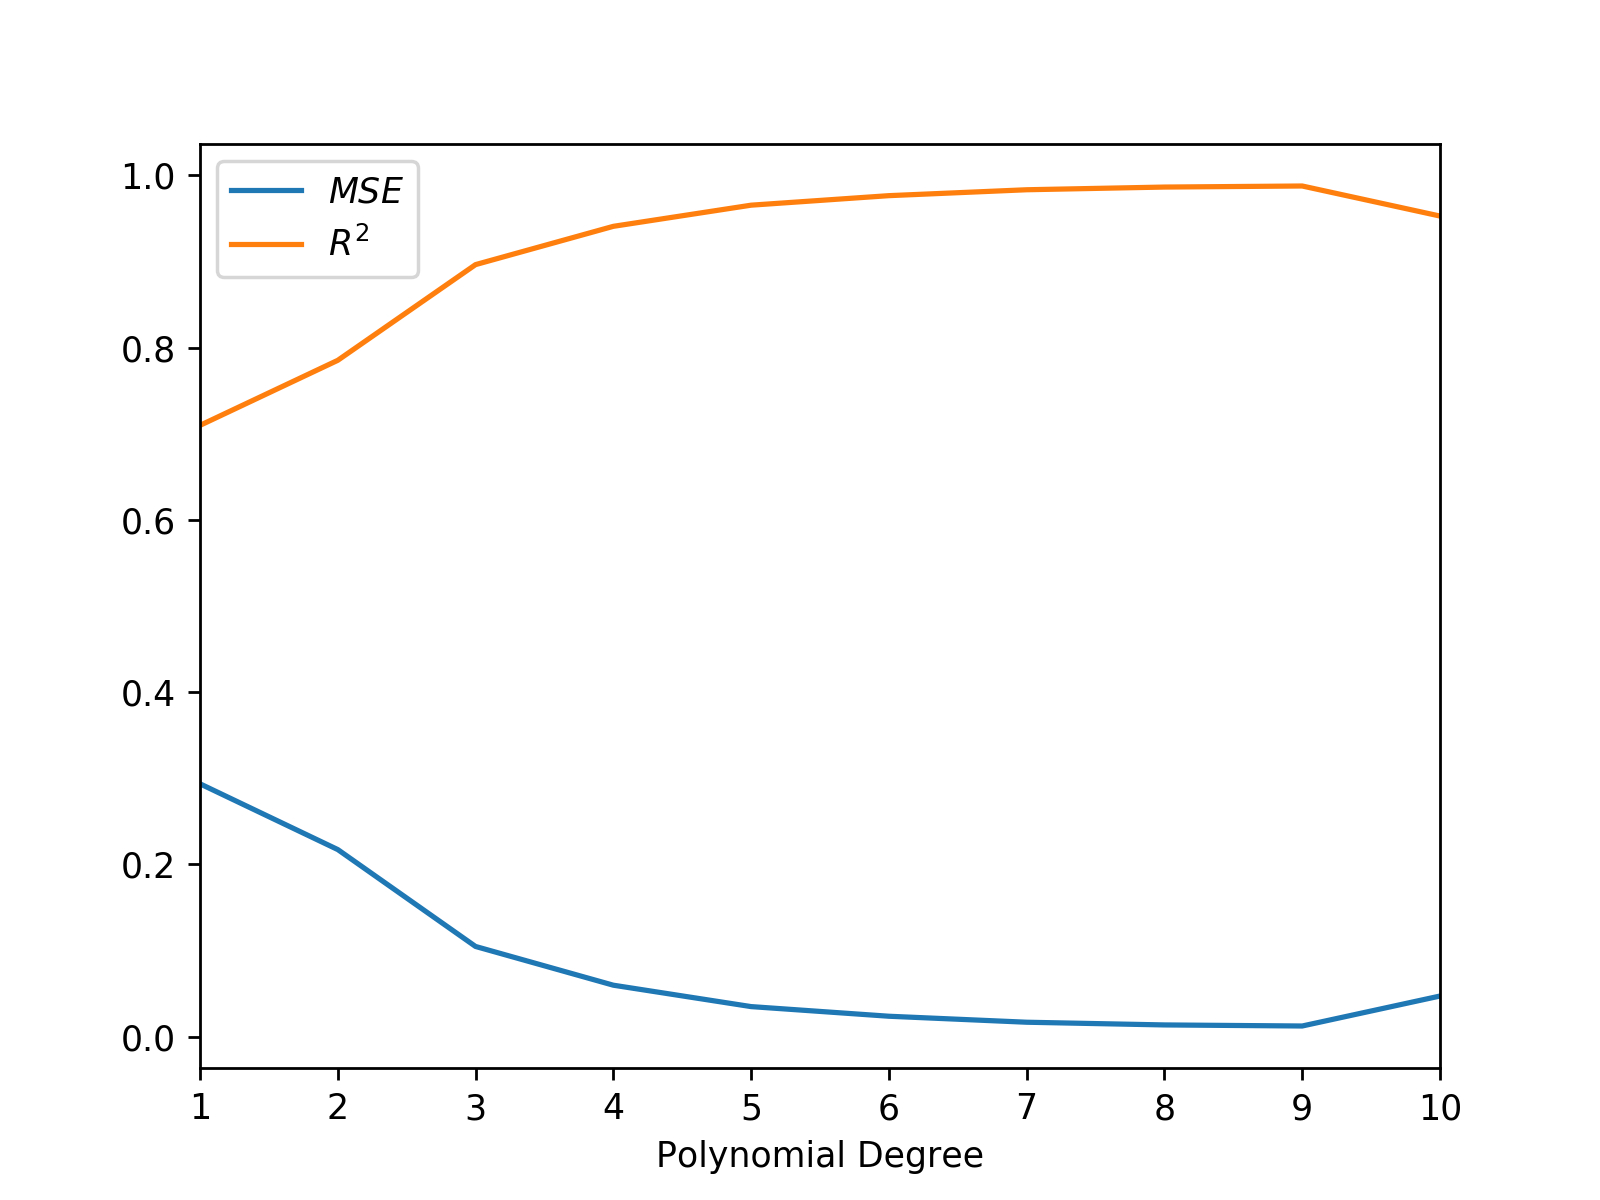
\includegraphics[width = 0.5\textwidth, center]{../franke_output/part_B.png}
	\caption{The $MSE$, the $R^2$-score, and the variance $\sigma$ in the vector of coefficients $\beta$ as functions of the polynomial degree after performing \textit{OLS} on the Franke function.  Using 12-fold cross validation.}
	\label{fig_5}
\end{figure}

\begin{figure}[H]
	\centering 
	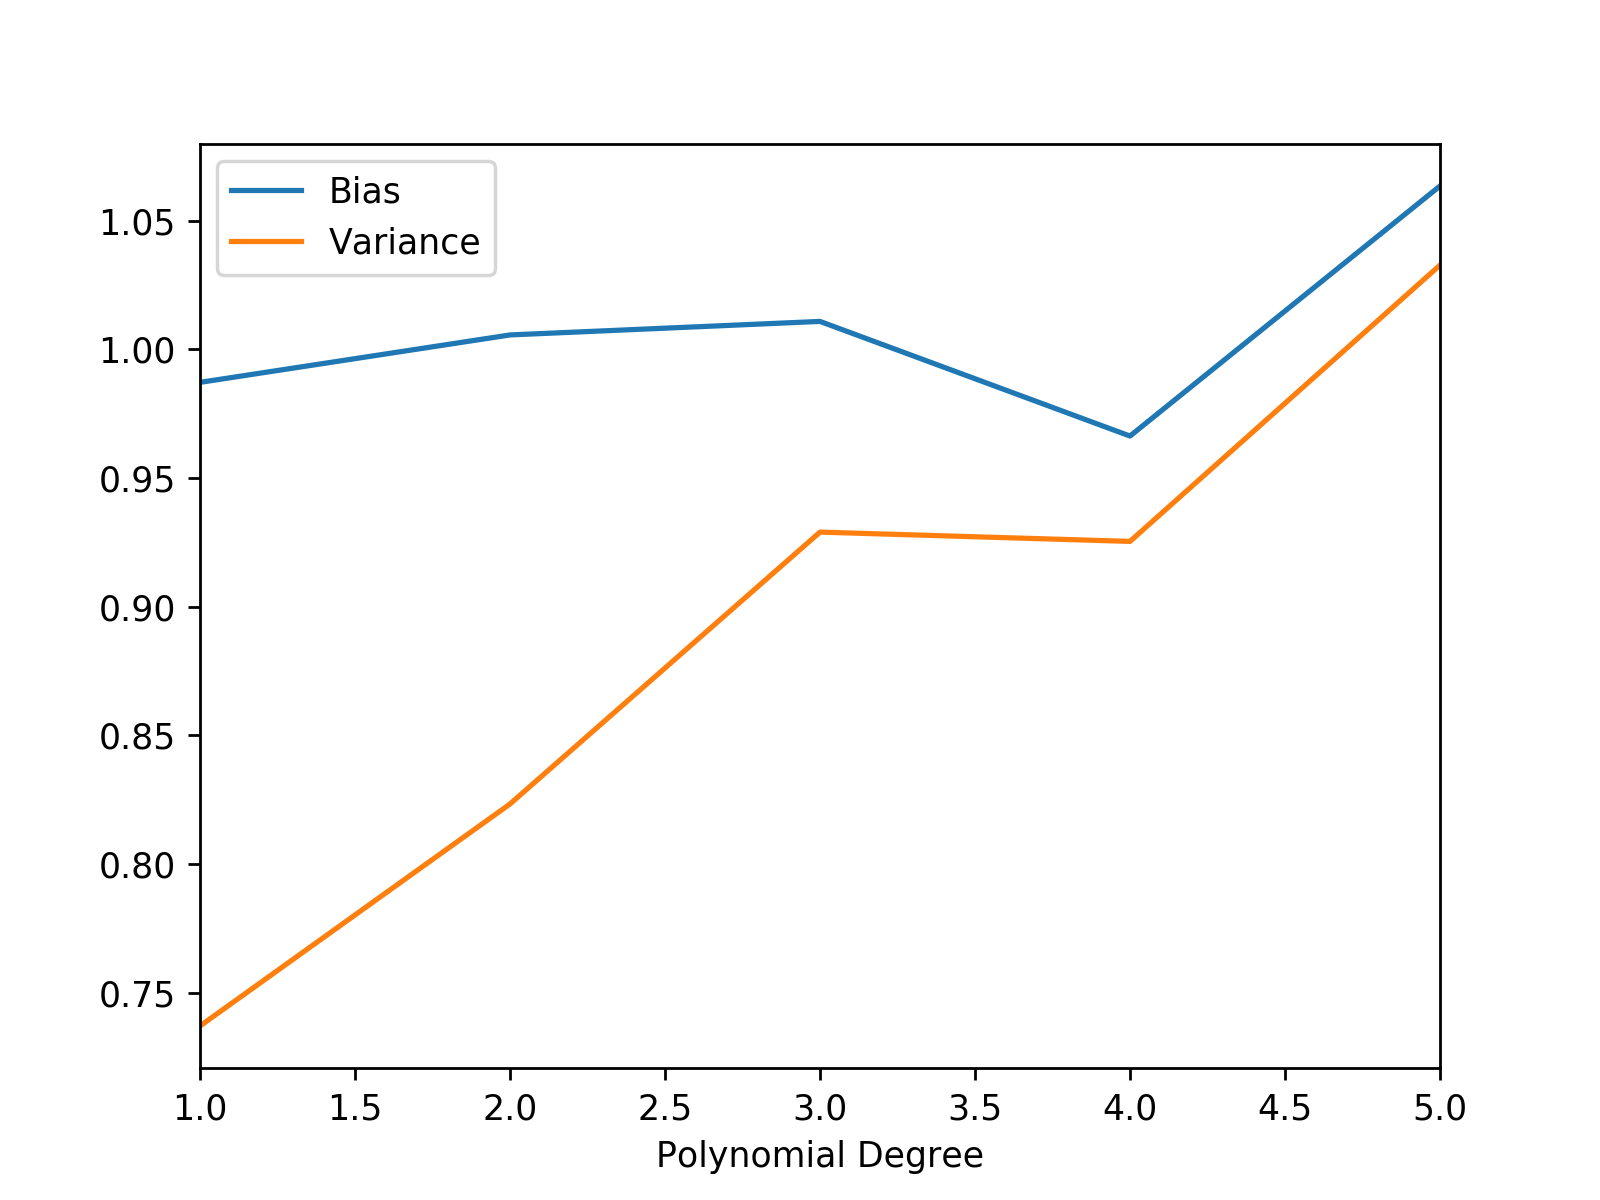
\includegraphics[width = 0.5\textwidth, center]{../franke_output/part_C_1.png}
	\caption{The \textit{bias} and \textit{variance} as functions of the polynomial degree after performing \textit{OLS} on the Franke function}
	\label{fig_6}
\end{figure}

\begin{figure}[H]
	\centering 
	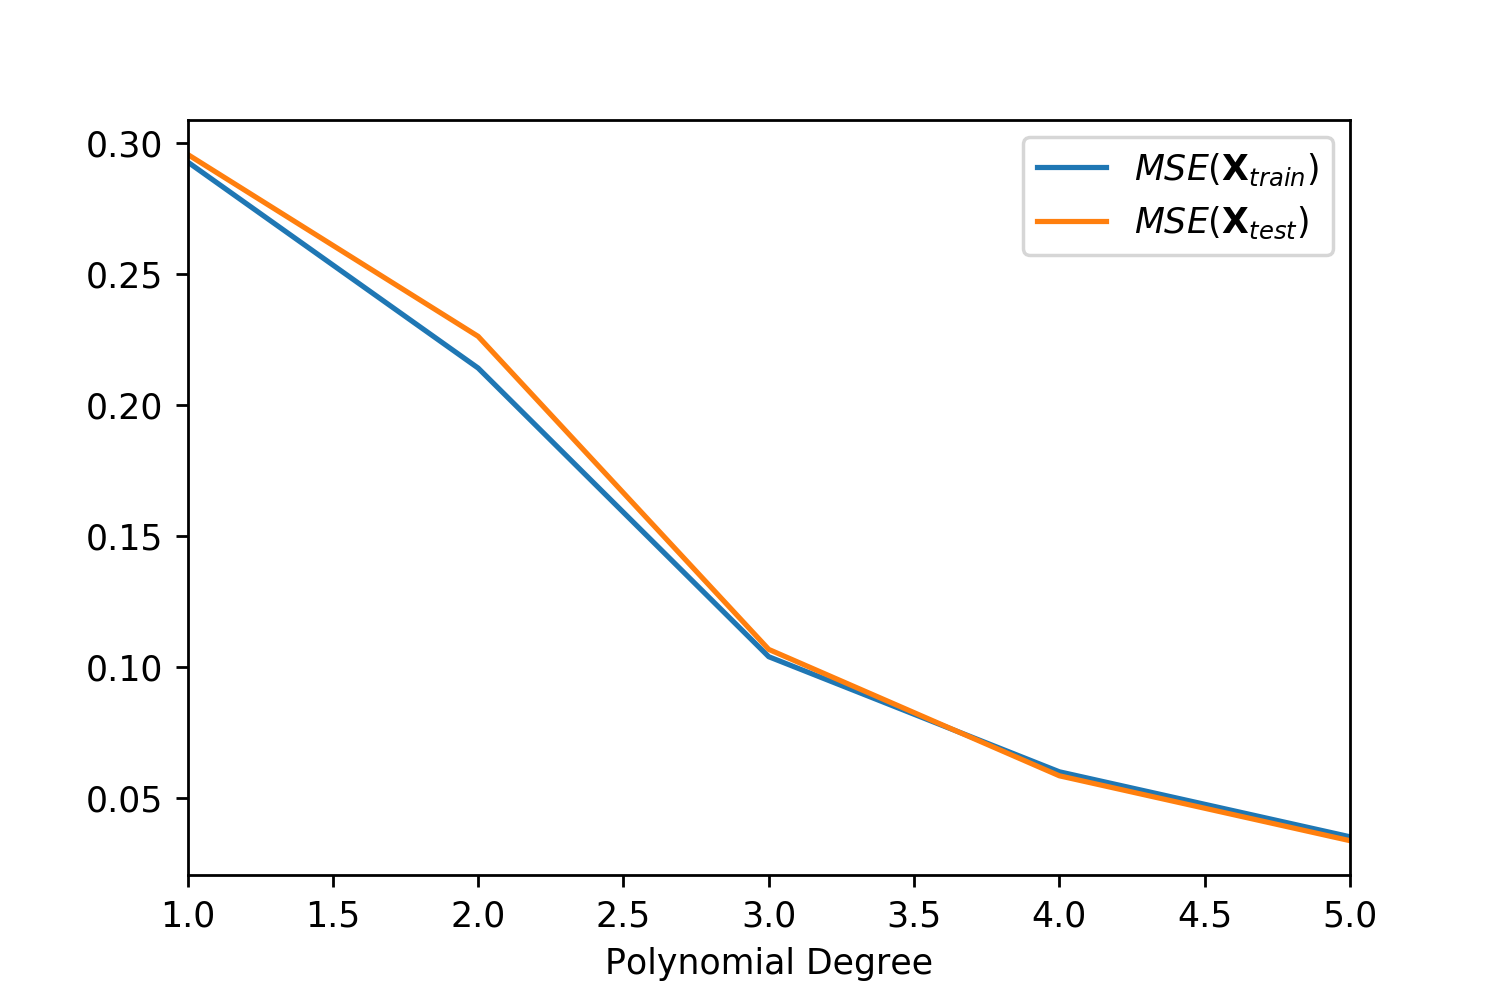
\includegraphics[width = 0.5\textwidth, center]{../franke_output/part_C_2.png}
	\caption{The $MSE$ for the \textit{training data} and the \textit{testing data}, as a function of the polynomial degree after performing \textit{OLS} on the Franke function}
	\label{fig_7}
\end{figure}

\begin{figure}[H]
	\centering 
	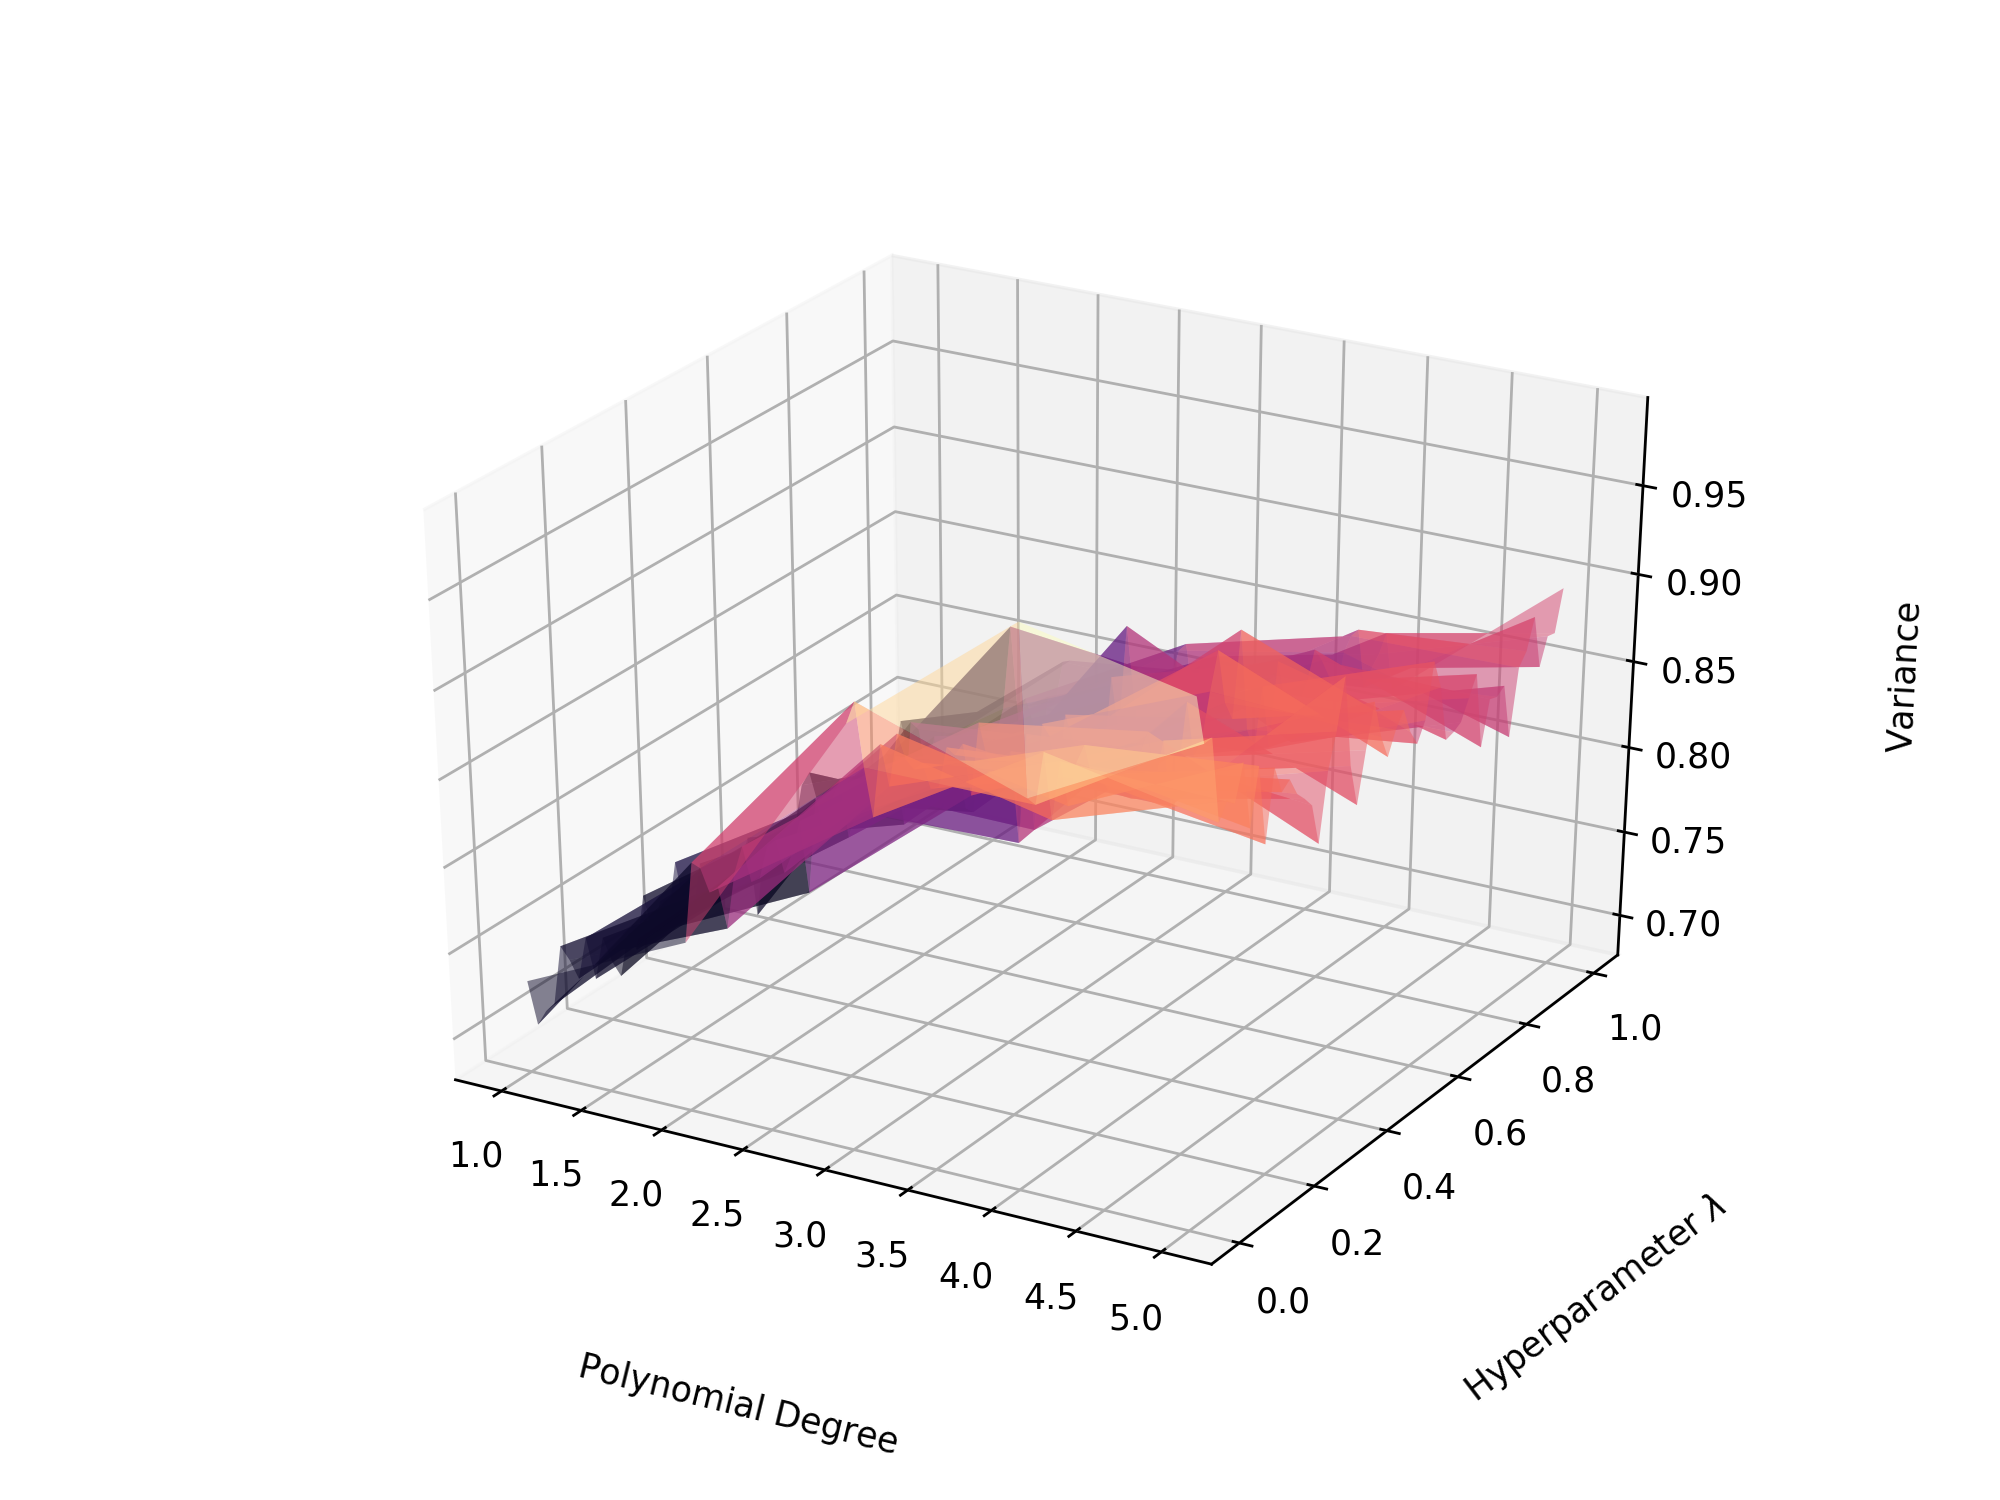
\includegraphics[width = 0.5\textwidth, center]{../franke_output/part_D_1.png}
	\caption{The \textit{variance} as a function of polynomial degree and hyperparameter $\lambda$, after performing \textit{Ridge regression} on the Franke function}
	\label{fig_8}
\end{figure}

\begin{figure}[H]
	\centering 
	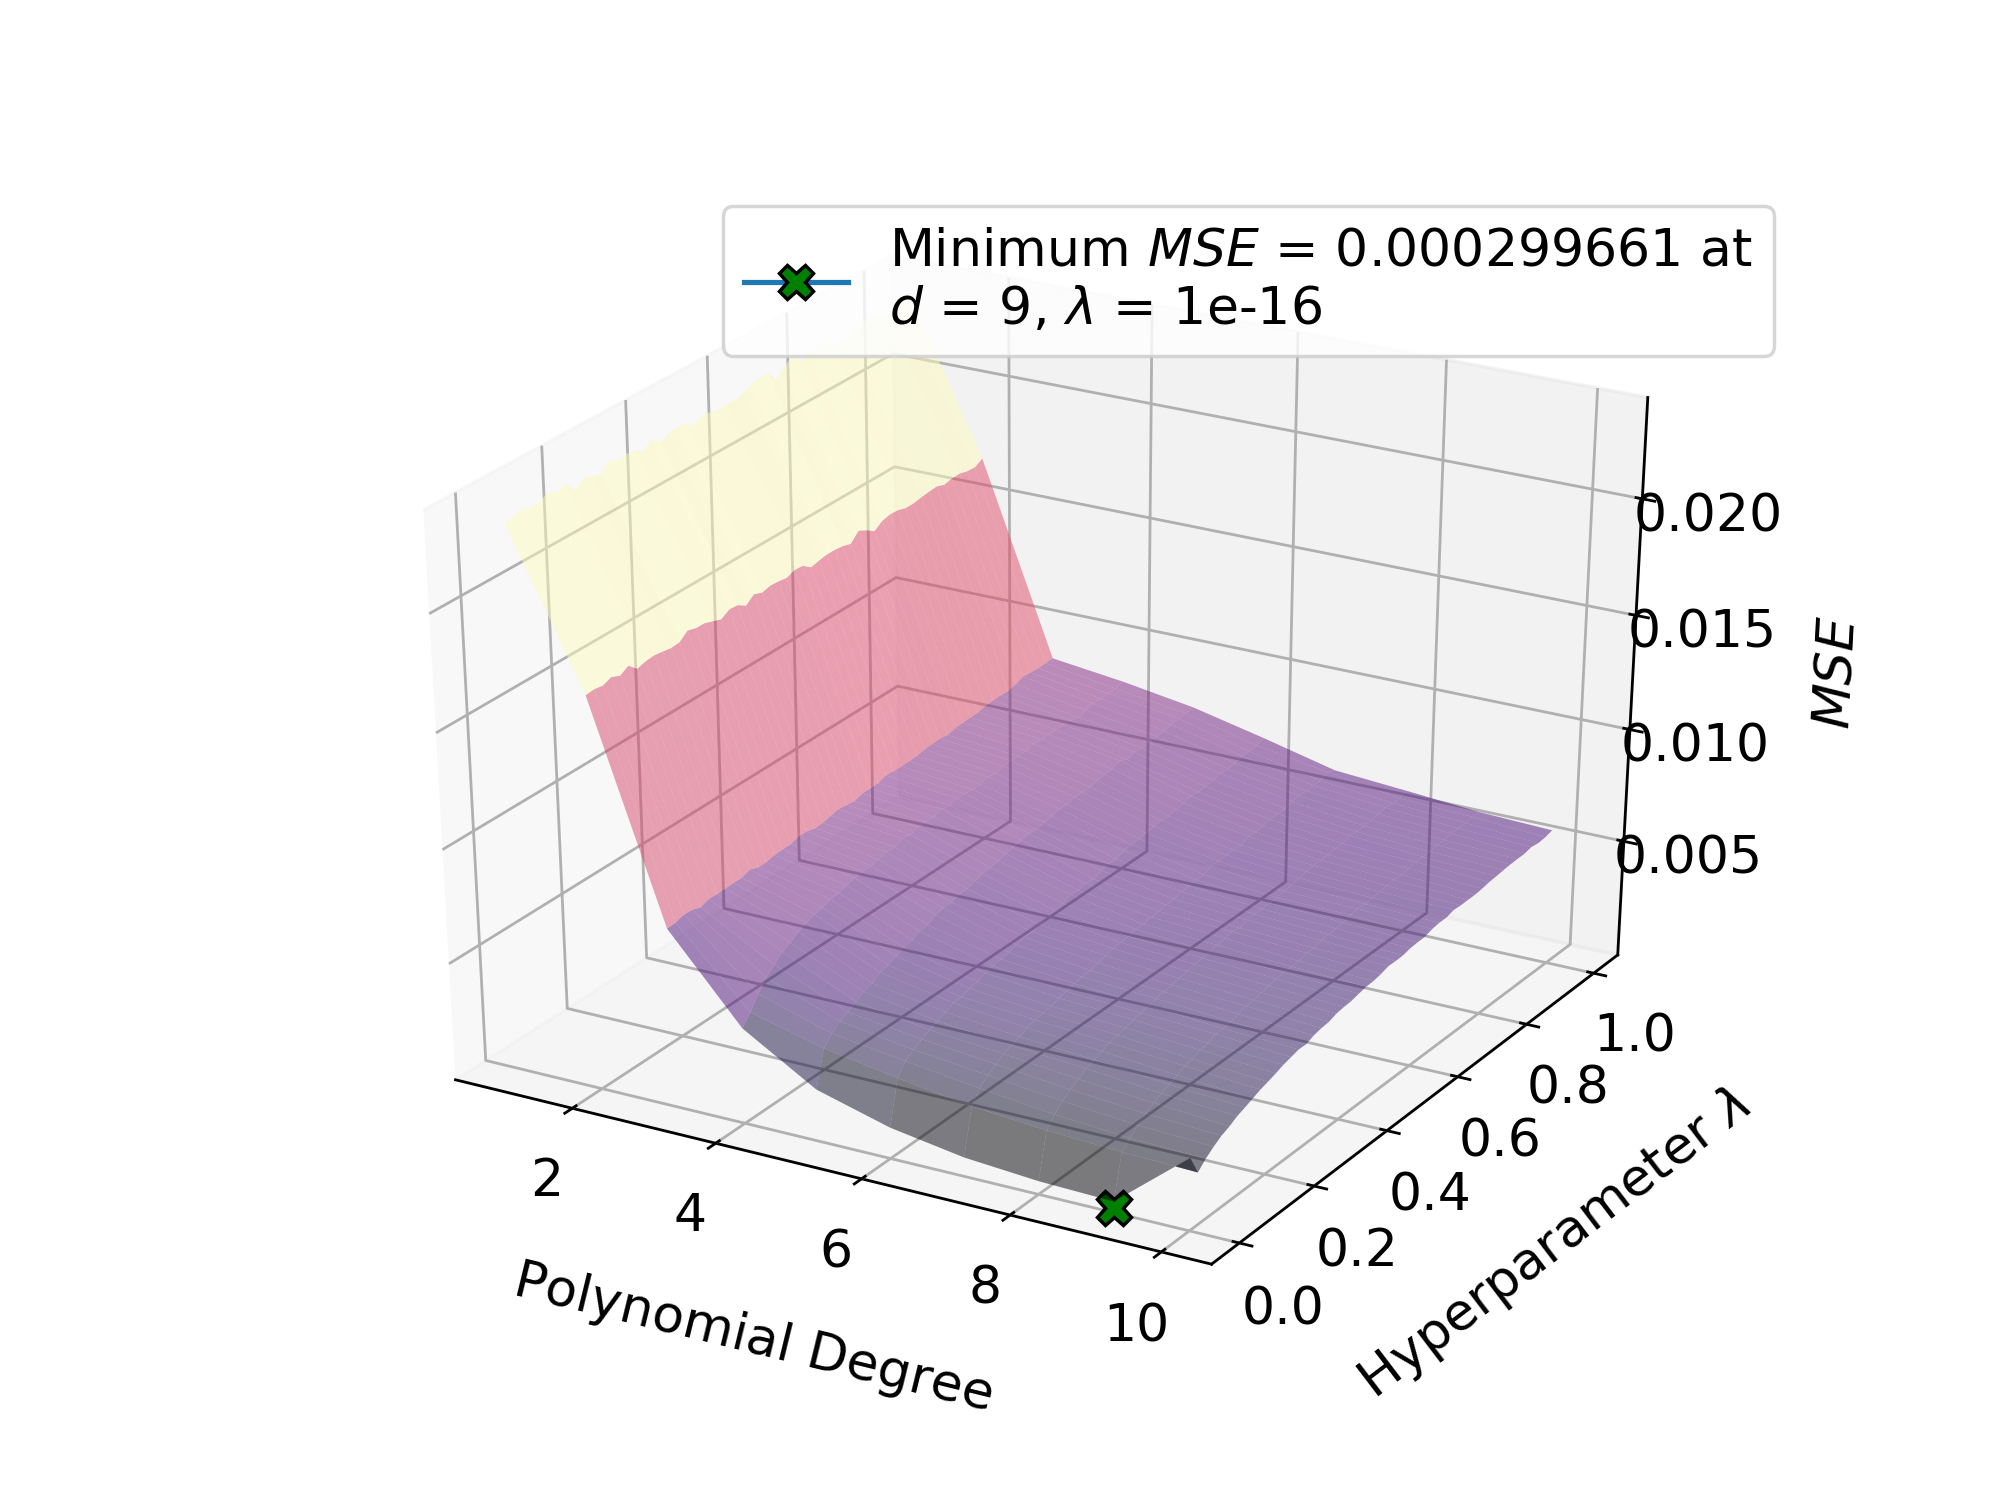
\includegraphics[width = 0.5\textwidth, center]{../franke_output/part_D_2.png}
	\caption{The $MSE$ as a function of the polynomial degree and hyperparameter $\lambda$ after performing \textit{Ridge regression} on the Franke function}
	\label{fig_9}
\end{figure}

\begin{figure}[H]
	\centering 
	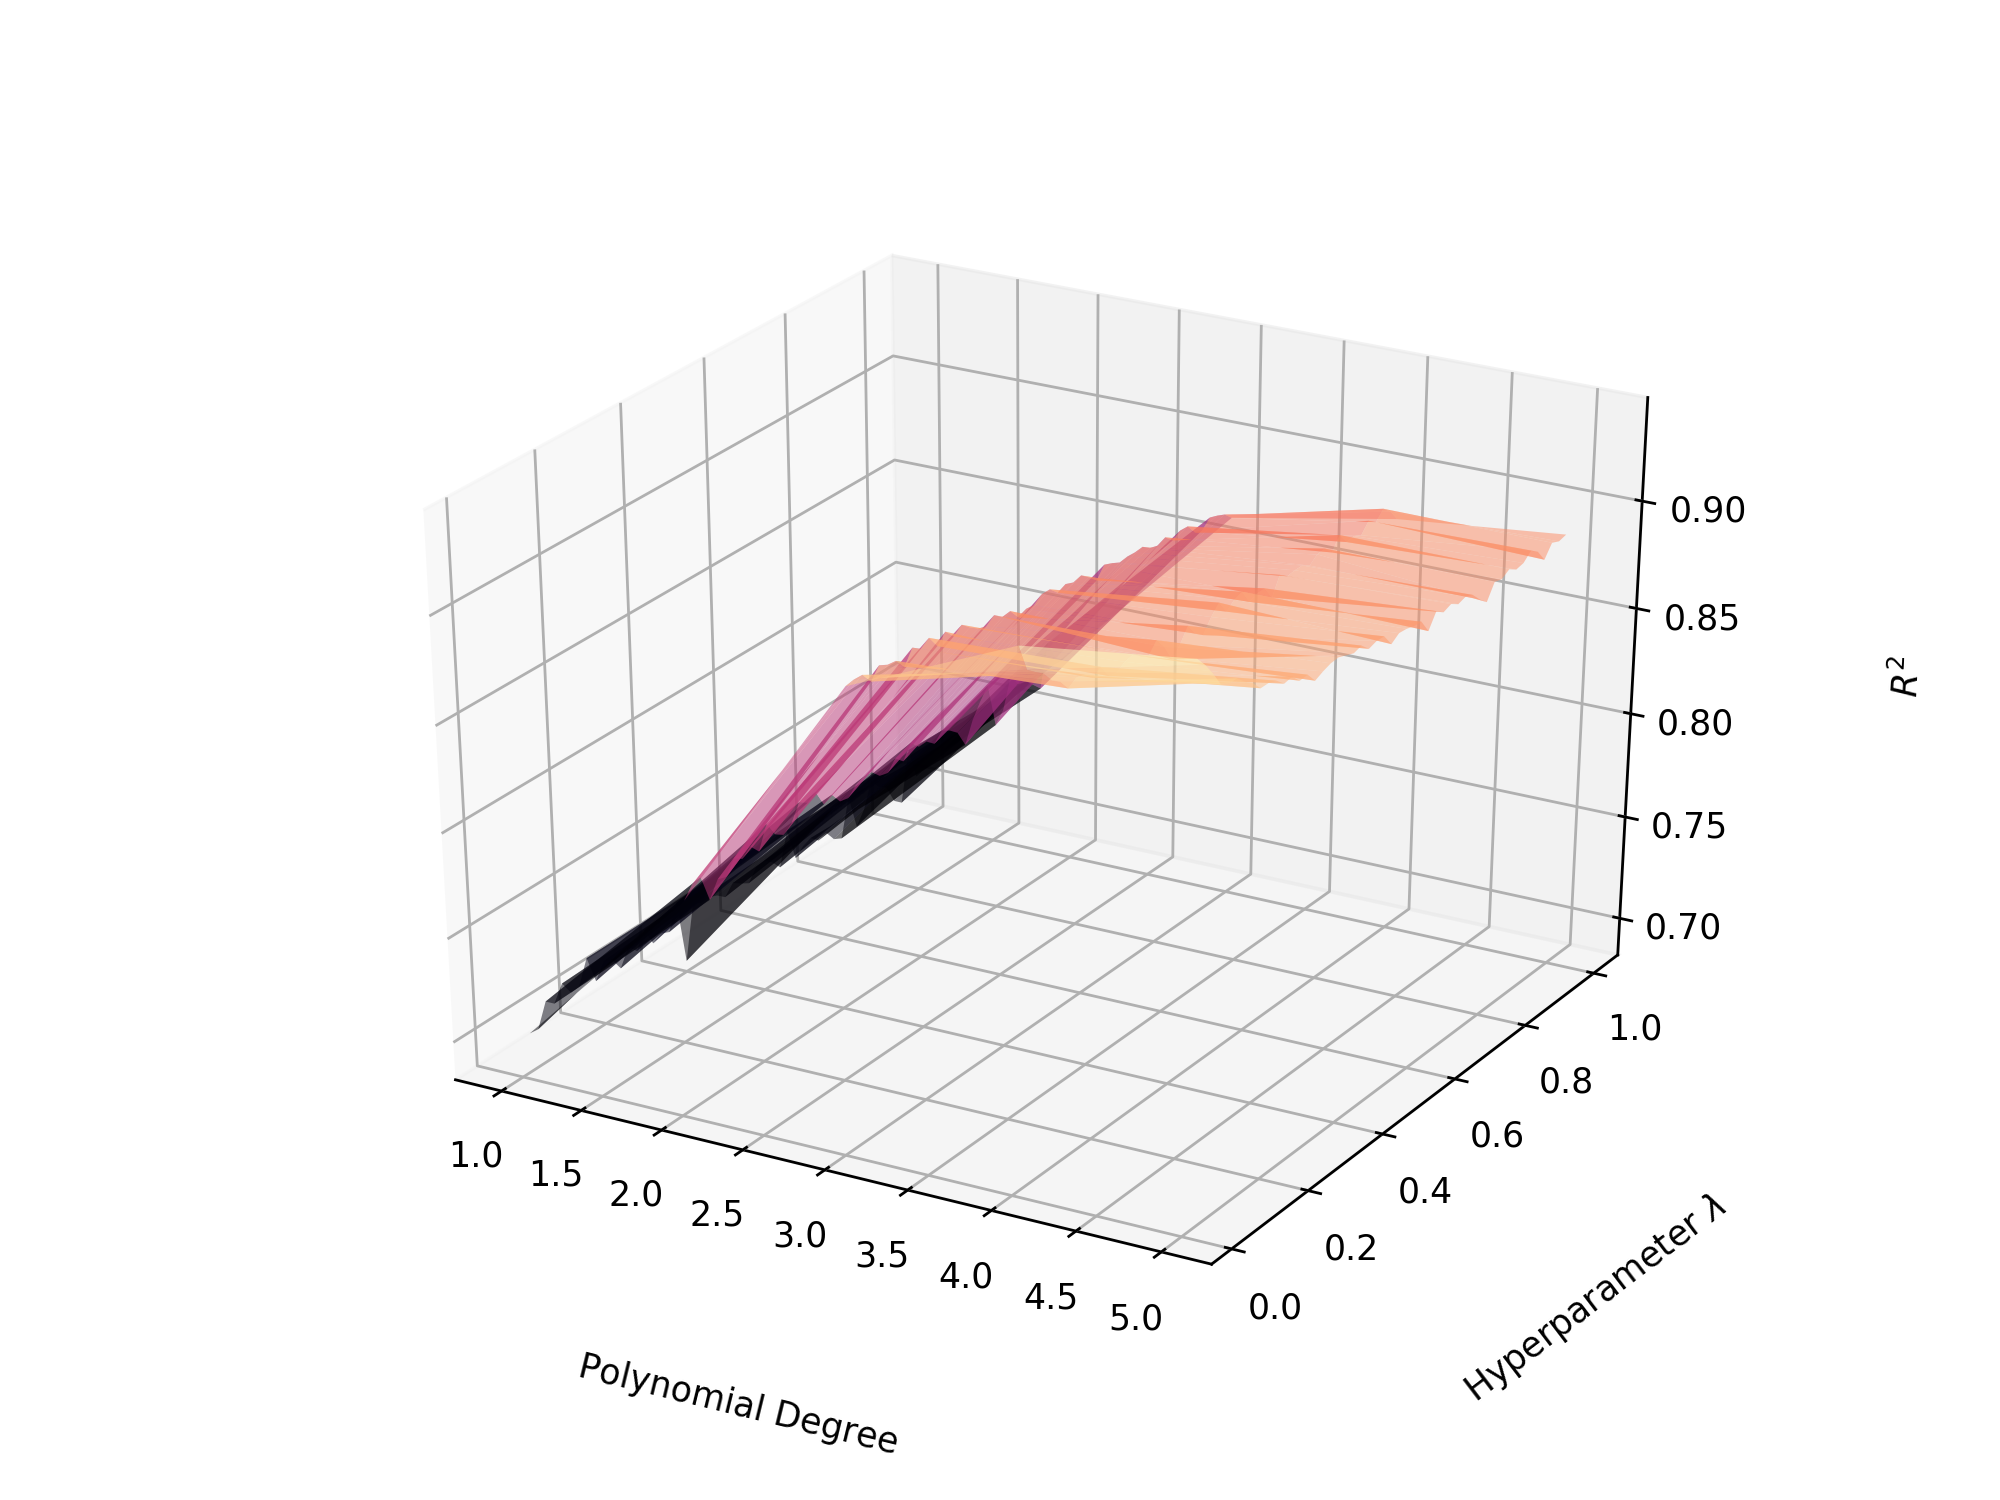
\includegraphics[width = 0.5\textwidth, center]{../franke_output/part_D_3.png}
	\caption{The $R^2$-score as a function of the polynomial degree and hyperparameter $\lambda$ after performing \textit{Ridge regression} on the Franke function}
	\label{fig_10}
\end{figure}

\begin{figure}[H]
	\centering 
	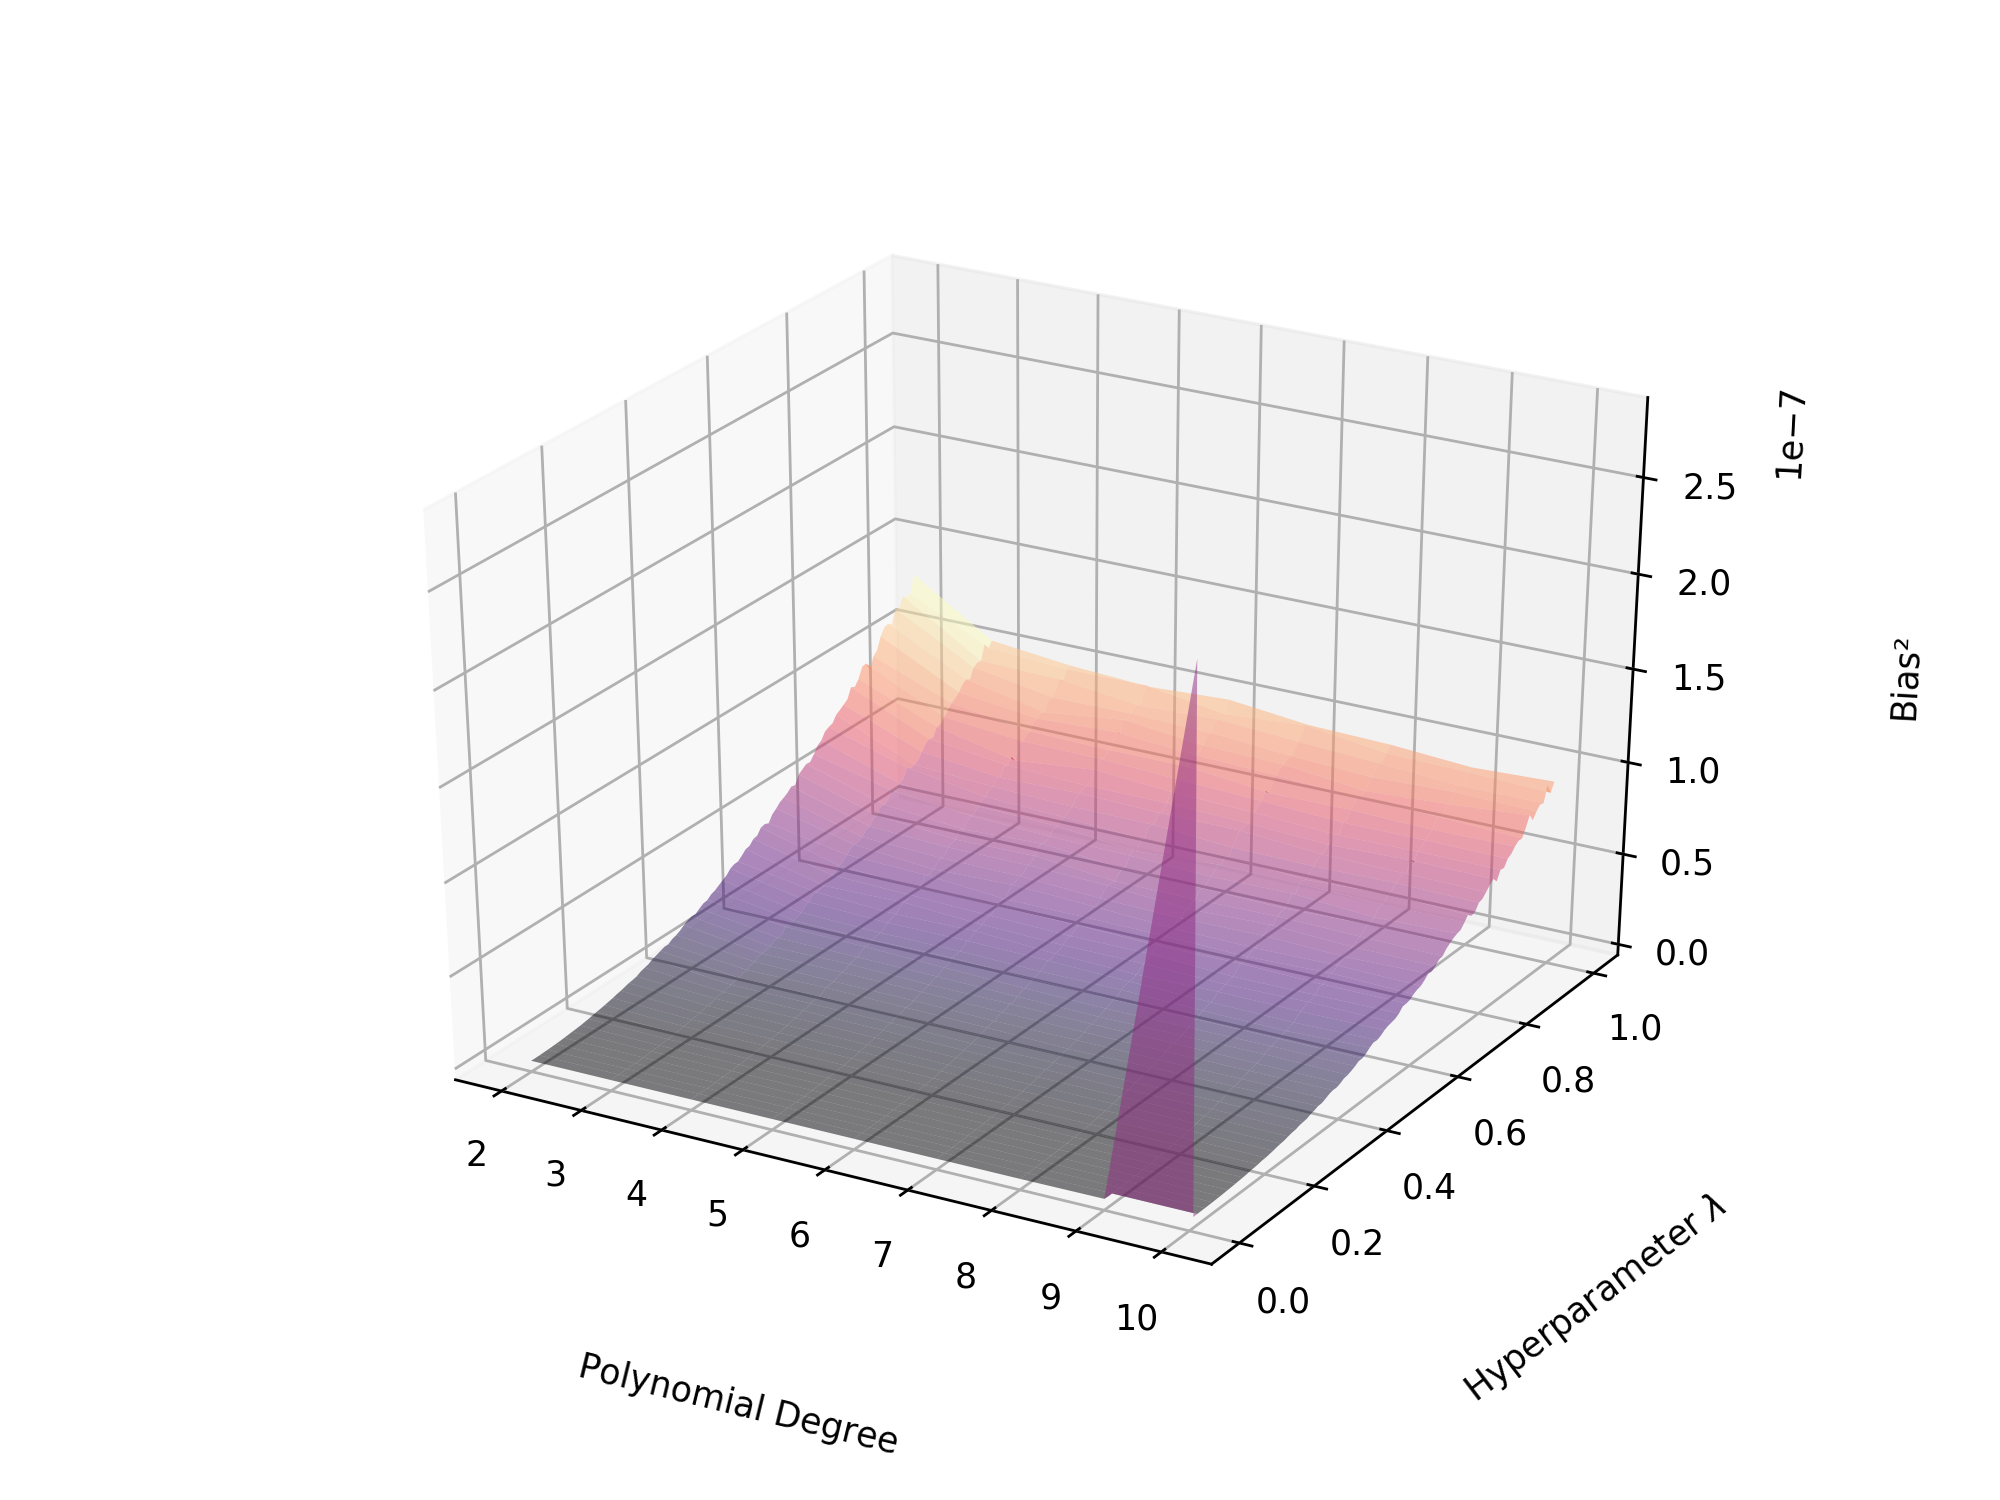
\includegraphics[width = 0.5\textwidth, center]{../franke_output/part_D_4.png}
	\caption{The \textit{squared bias} as a function of the polynomial degree and hyperparameter $\lambda$ after performing \textit{Ridge regression} on the Franke function}
	\label{fig_11}
\end{figure}

\begin{figure}[H]
	\centering 
	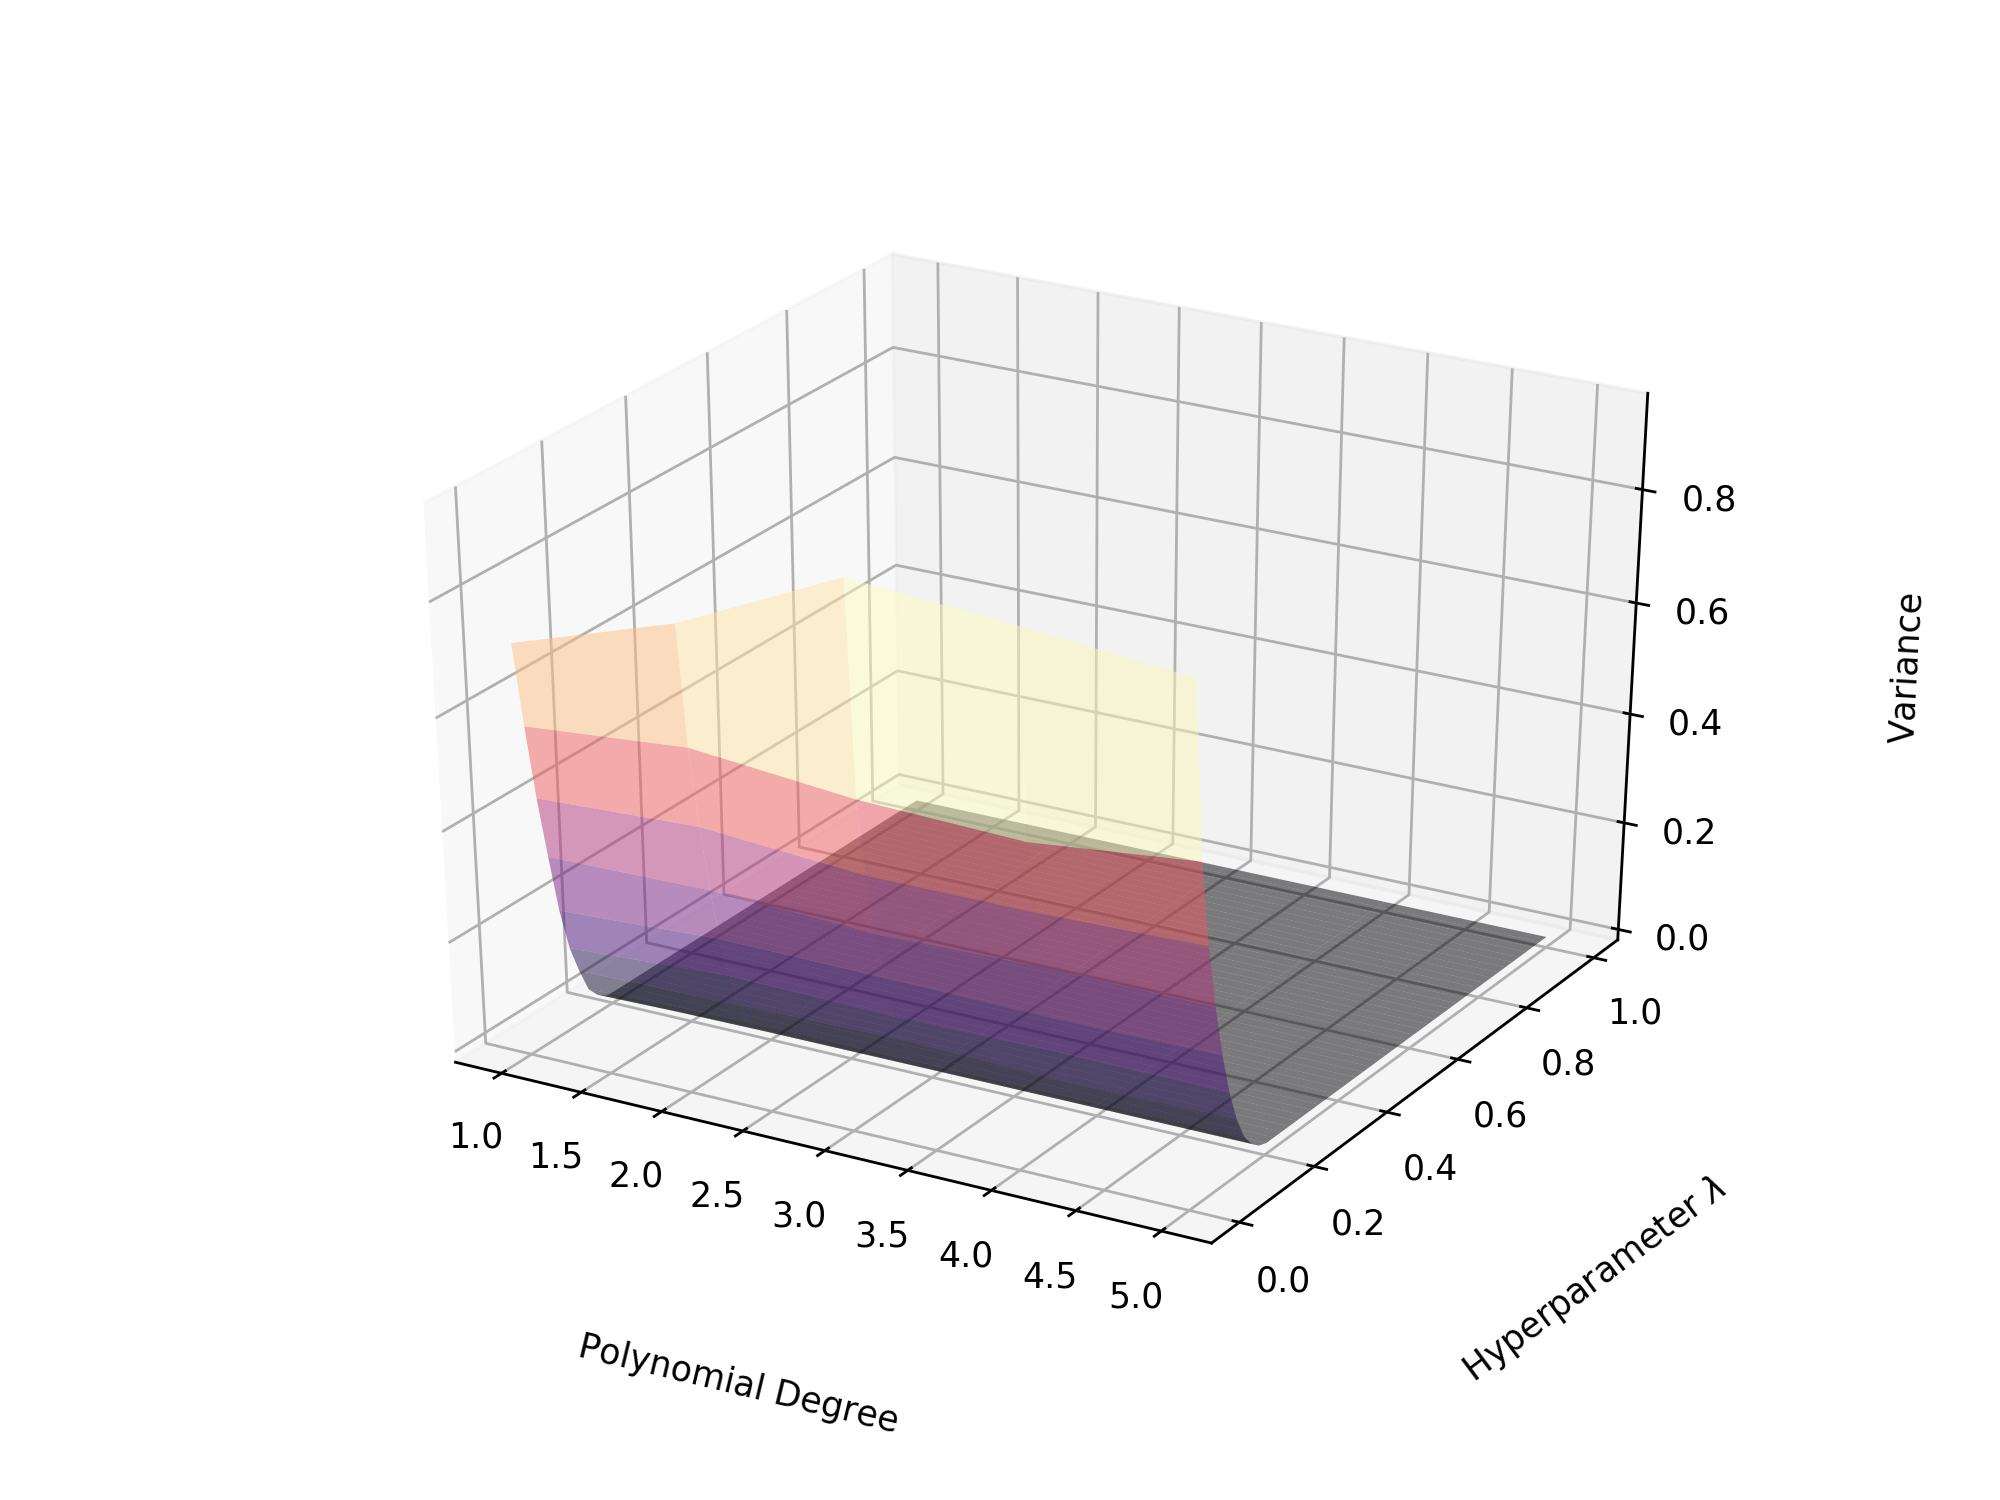
\includegraphics[width = 0.5\textwidth, center]{../franke_output/part_E_1.png}
	\caption{The \textit{variance} as a function of the polynomial degree and hyperparameter $\lambda$ after performing \textit{\textsc{lasso} regression} on the Franke function}
	\label{fig_12}
\end{figure}

\begin{figure}[H]
	\centering 
	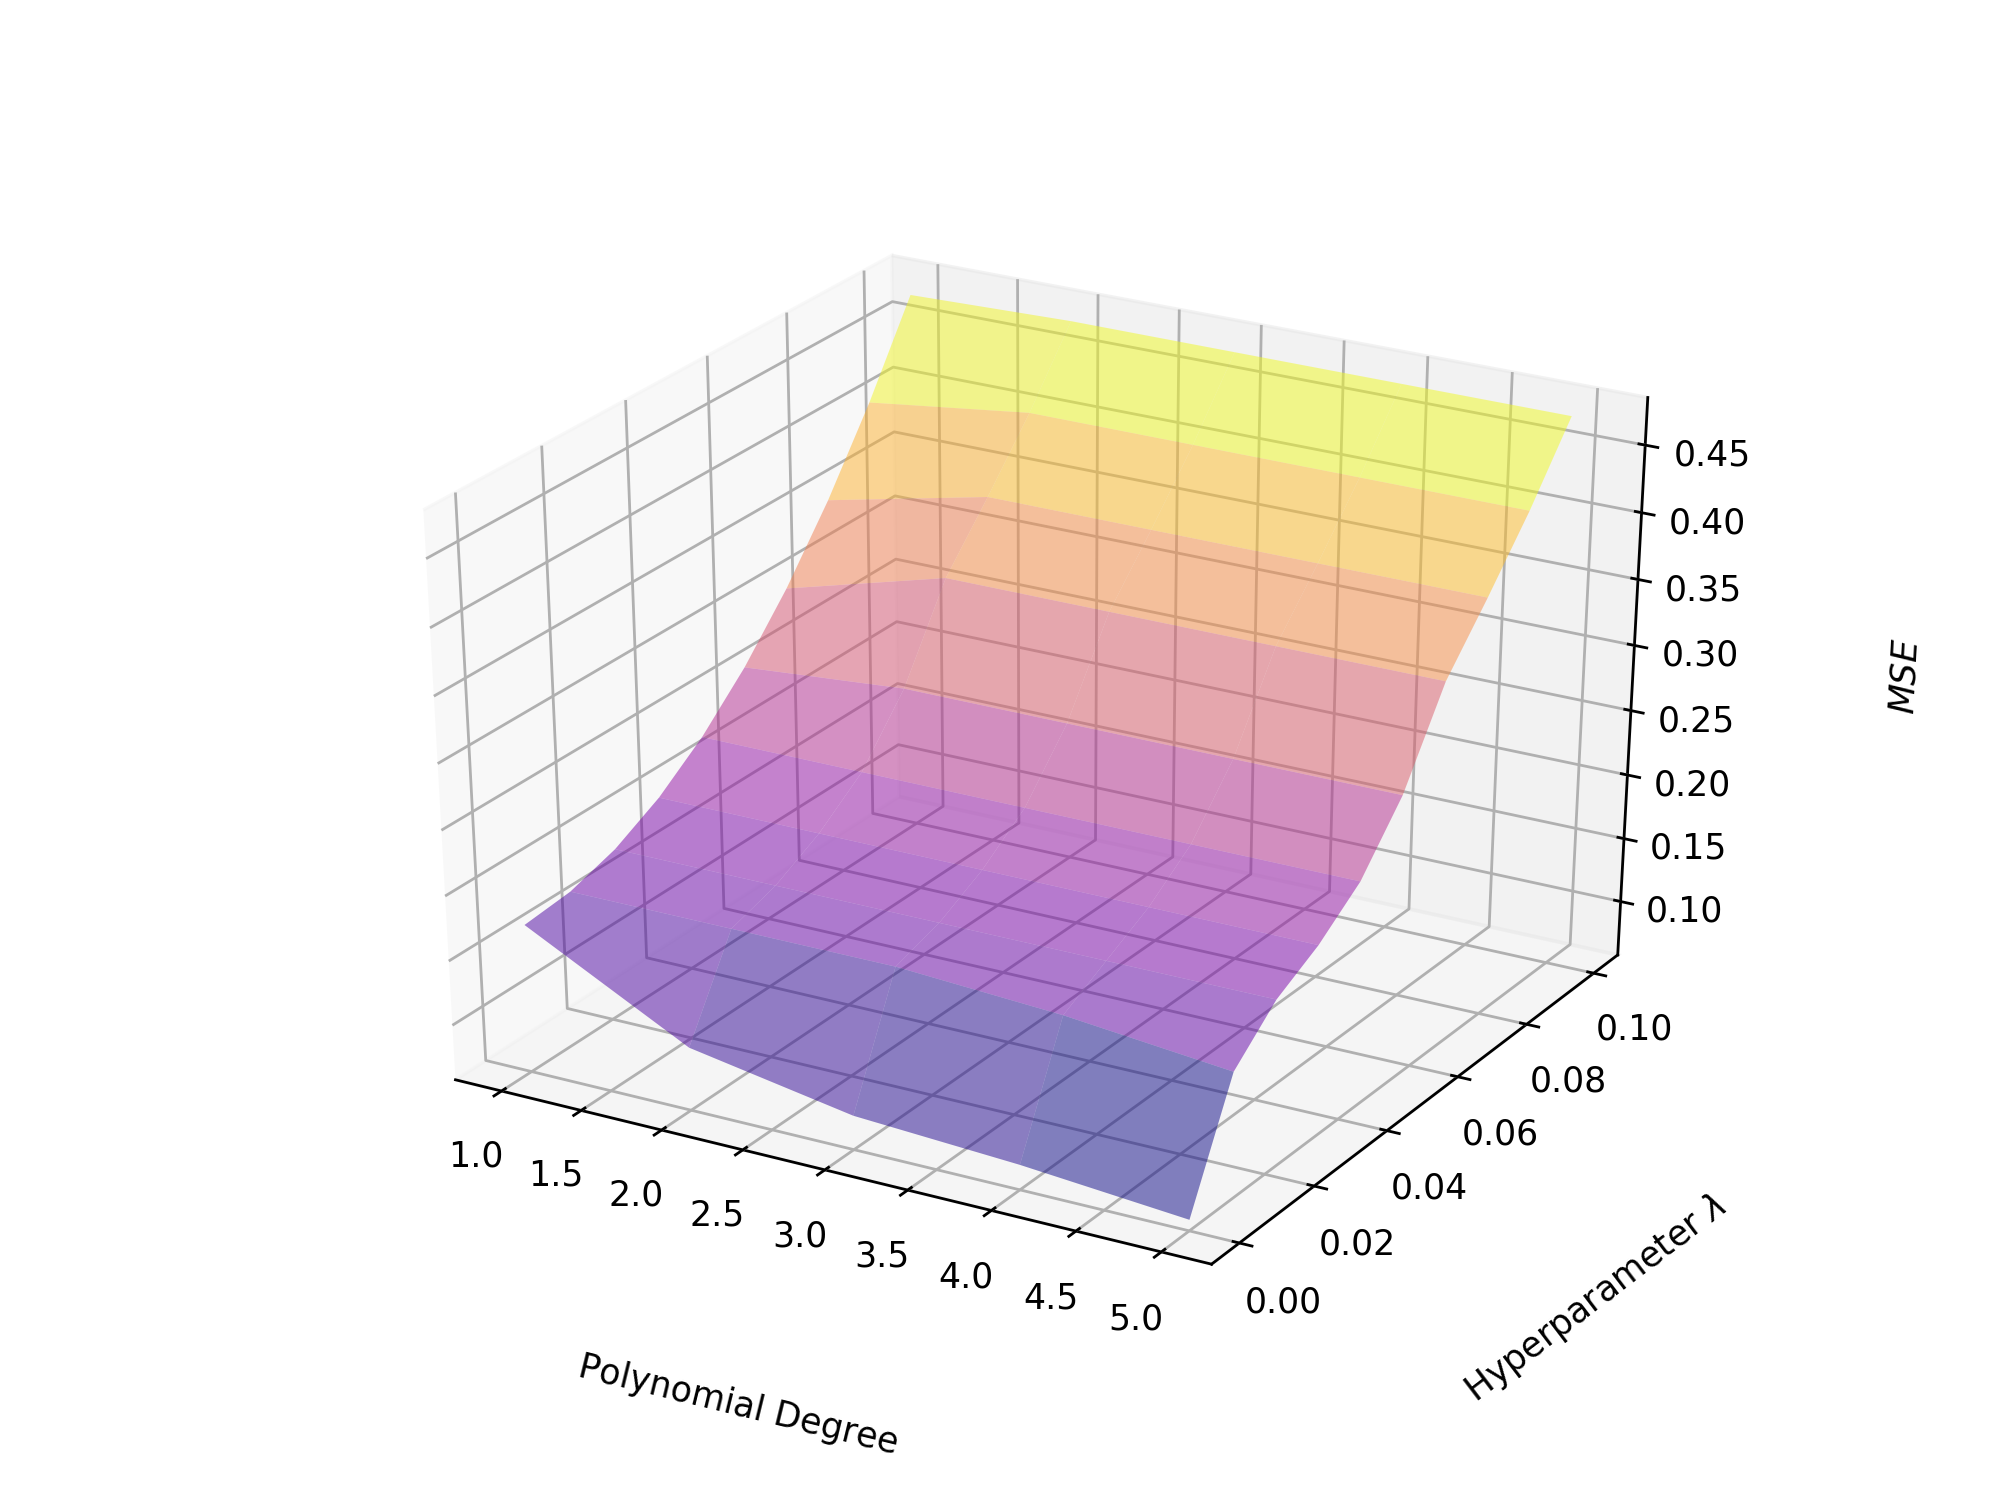
\includegraphics[width = 0.5\textwidth, center]{../franke_output/part_E_2.png}
	\caption{The $MSE$ as a function of the polynomial degree and hyperparameter $\lambda$ after performing \textit{\textsc{lasso} regression} on the Franke function}
	\label{fig_13}
\end{figure}

\begin{figure}[H]
	\centering 
	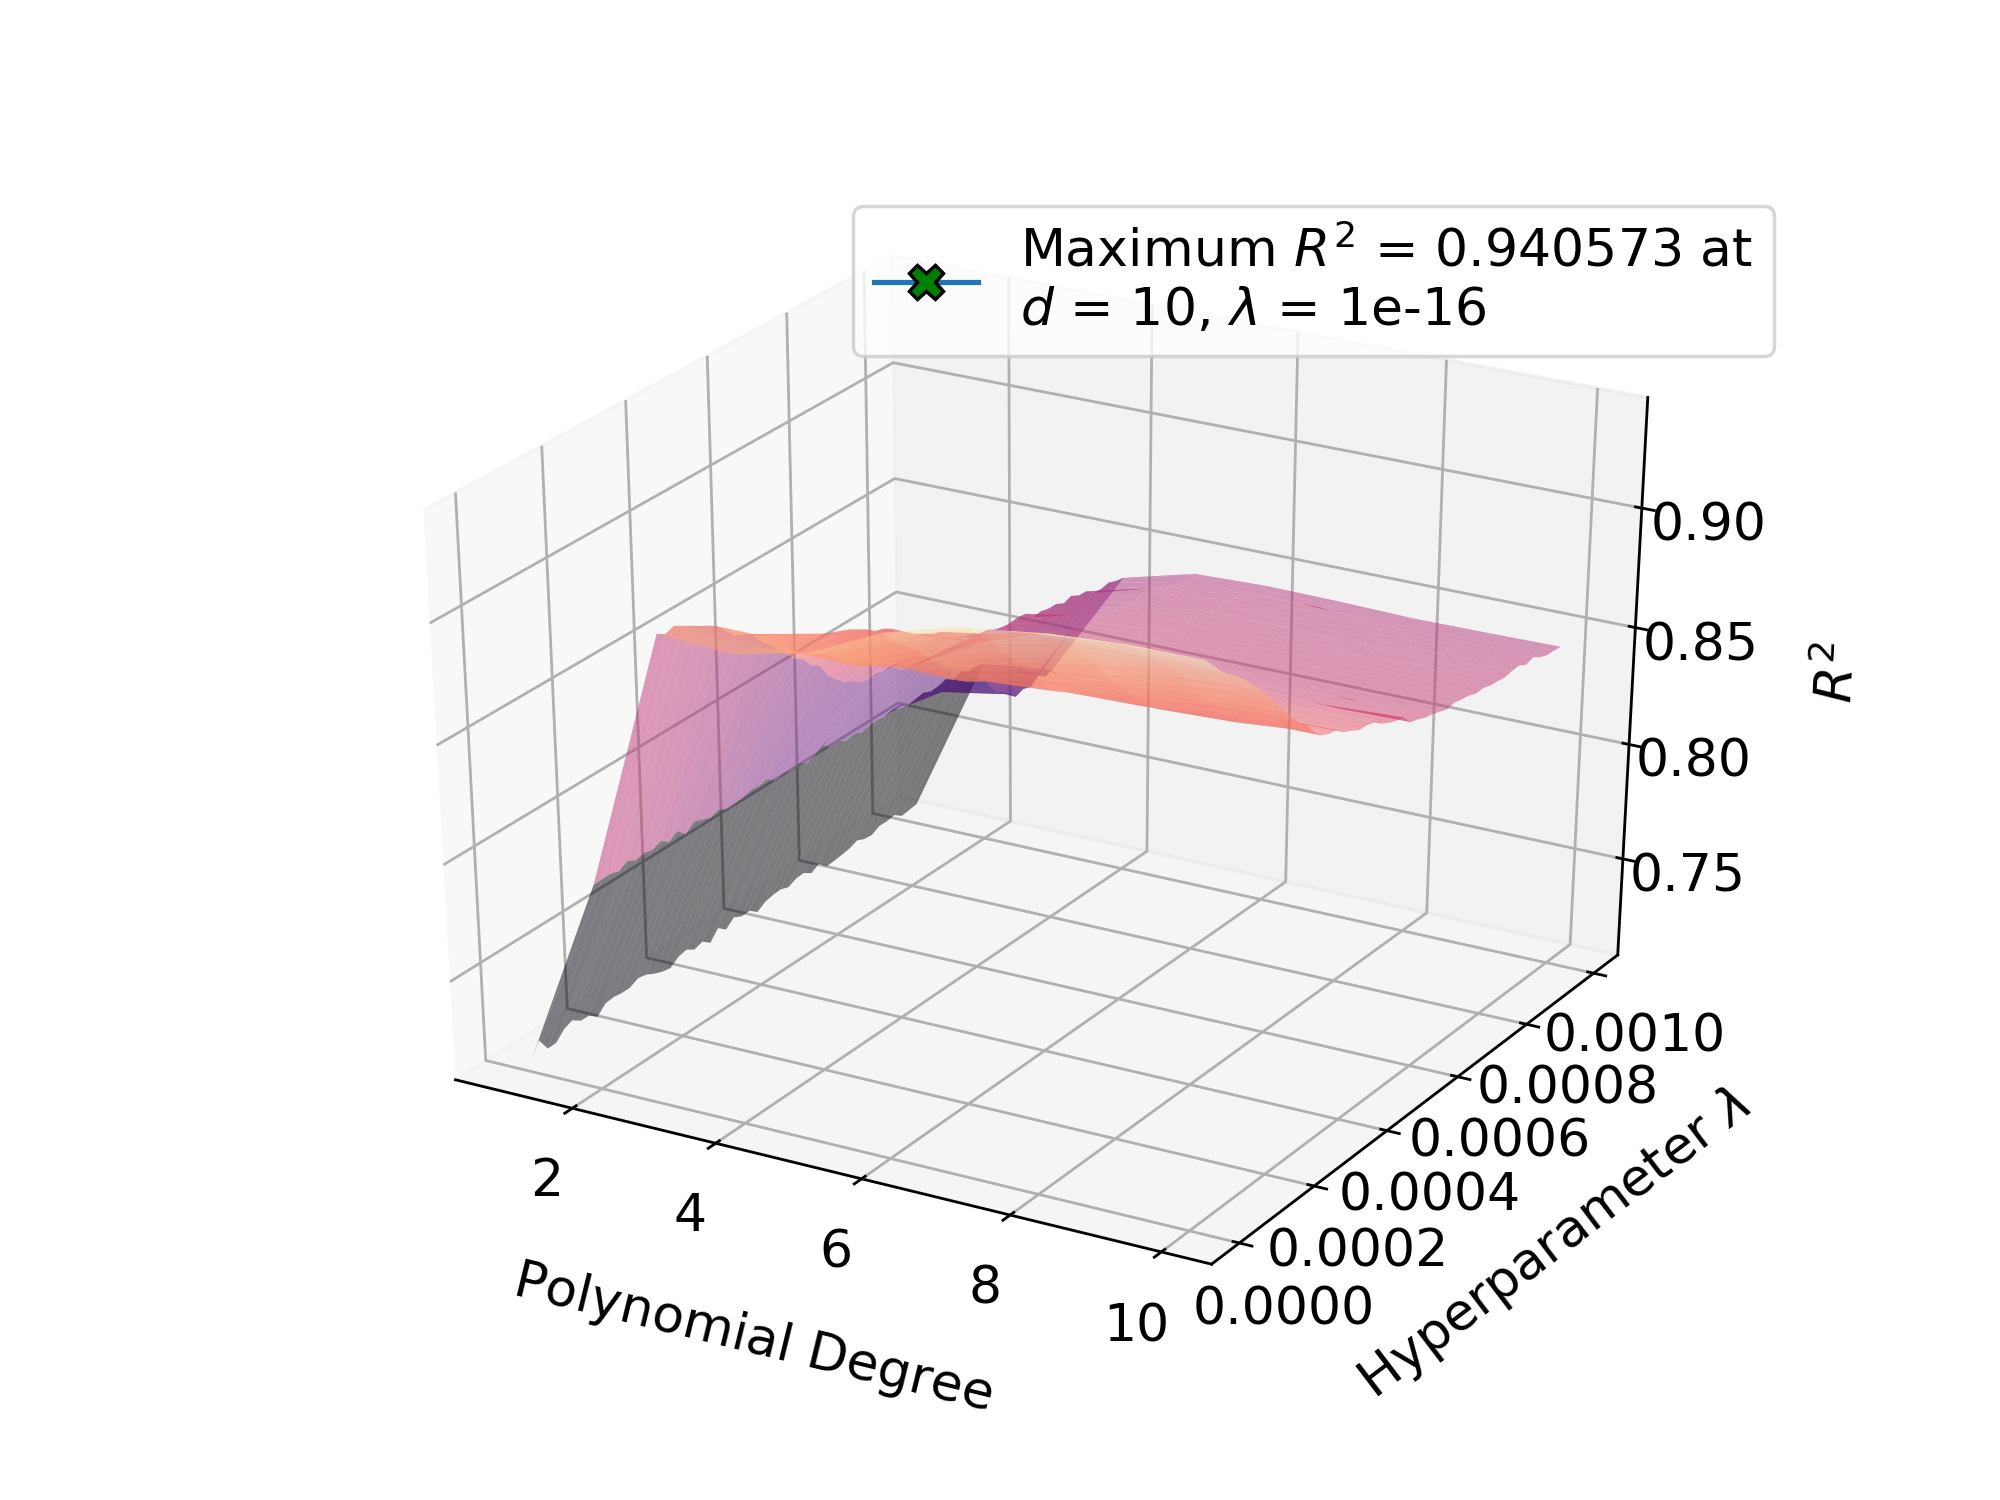
\includegraphics[width = 0.5\textwidth, center]{../franke_output/part_E_3.png}
	\caption{The $R^2$-score as a function of the polynomial degree and hyperparameter $\lambda$ after performing \textit{\textsc{lasso} regression} on the Franke function}
	\label{fig_14}
\end{figure}

\begin{figure}[H]
	\centering 
	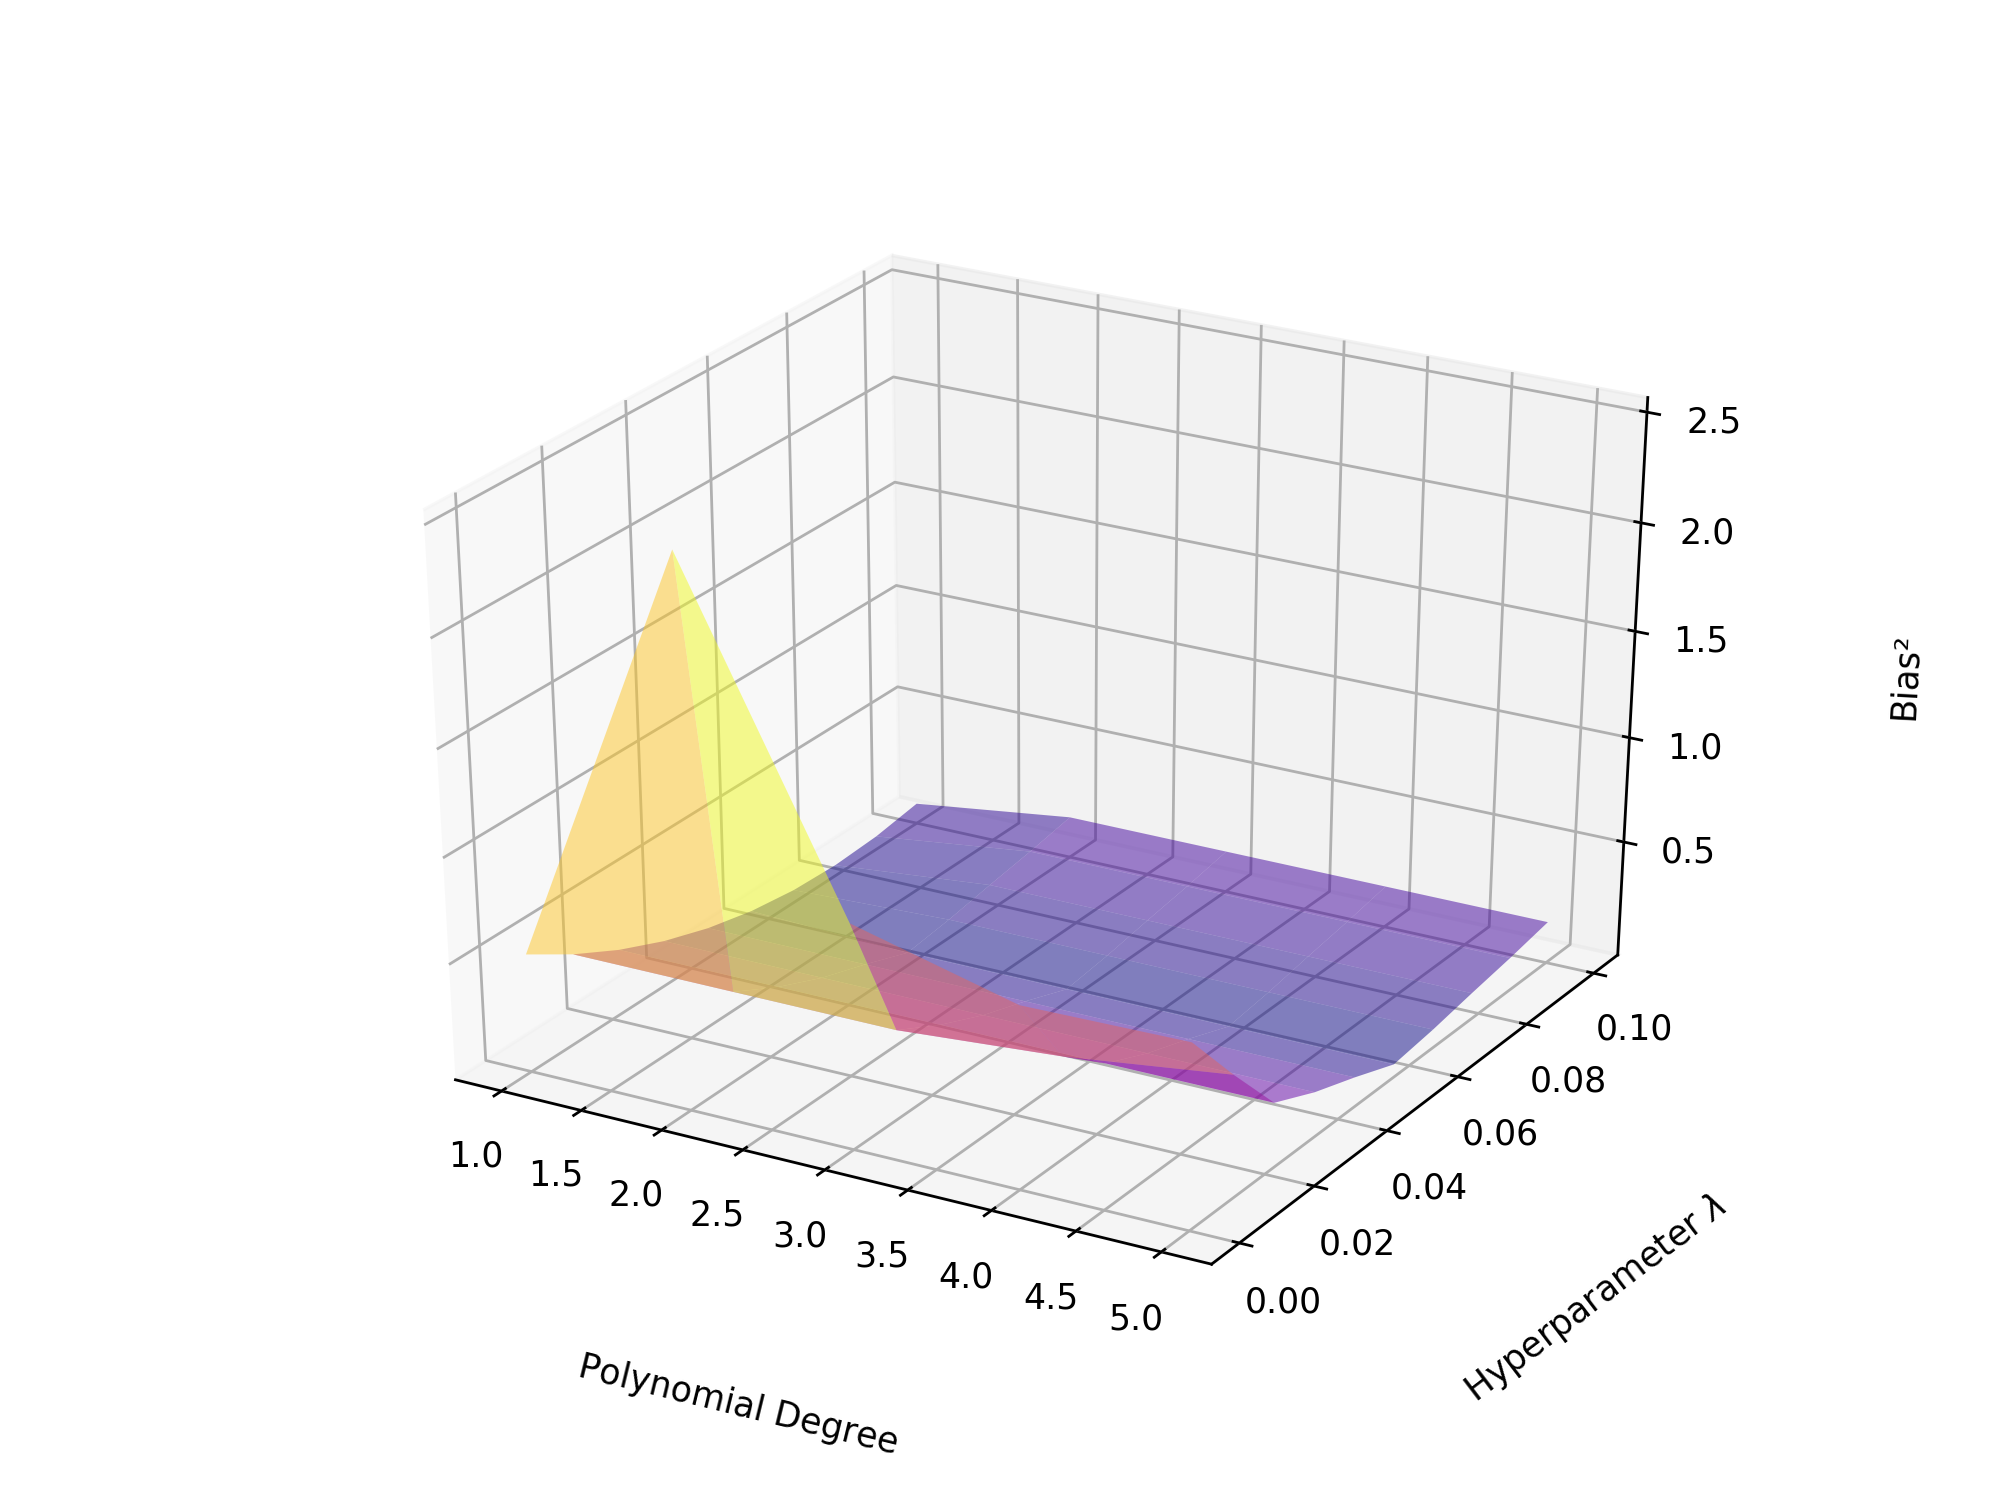
\includegraphics[width = 0.5\textwidth, center]{../franke_output/part_E_4.png}
	\caption{The \textit{squared bias} as a function of the polynomial degree and hyperparameter $\lambda$ after performing \textit{\textsc{lasso} regression} on the Franke function}
	\label{fig_15}
\end{figure}

\subsection*{Møsvatn Austfjell}

\begin{figure}[H]
	\centering 
	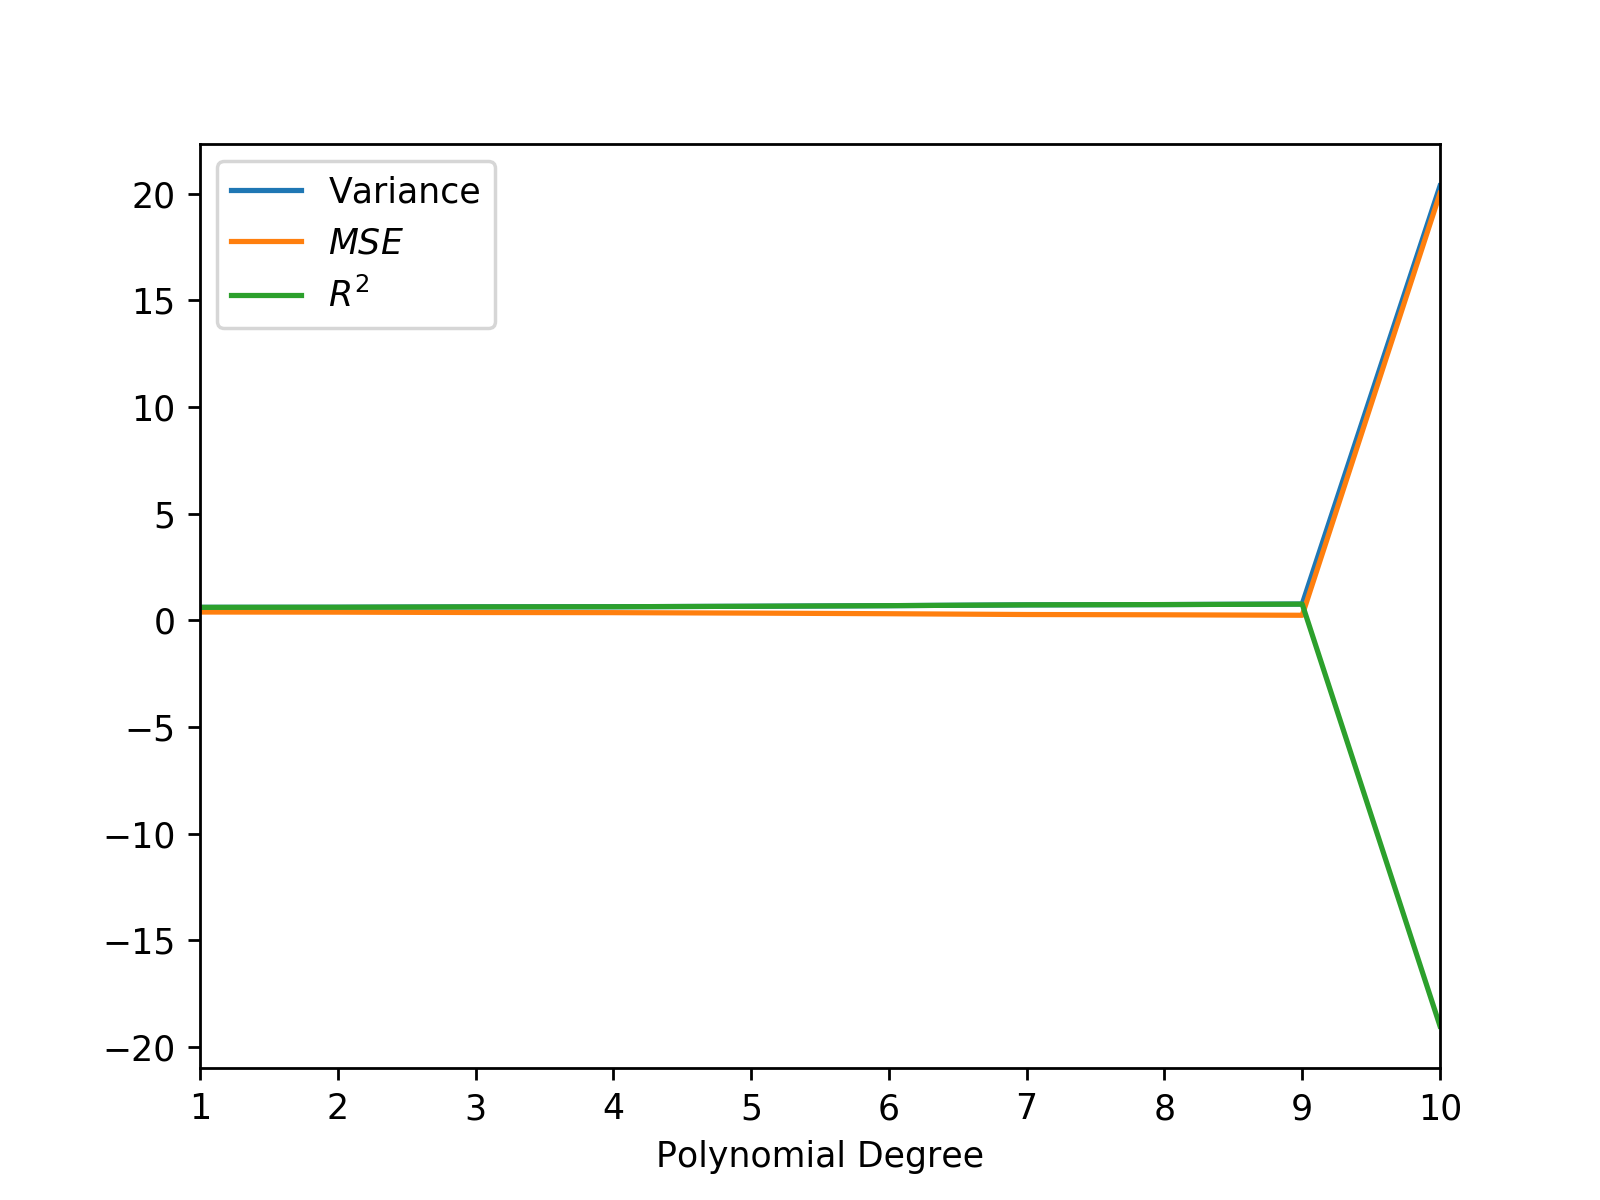
\includegraphics[width = 0.5\textwidth, center]{../real_output/part_A.png}
	\caption{The $MSE$, $R^2$-score and variance $\sigma$ of the vector of coefficients $\beta$ as a function of the polynomial degree after performing \textit{OLS} on real terrain data from \textit{Møsvatn Austfjell}}
	\label{fig_16}
\end{figure}

\begin{figure}[H]
	\centering 
	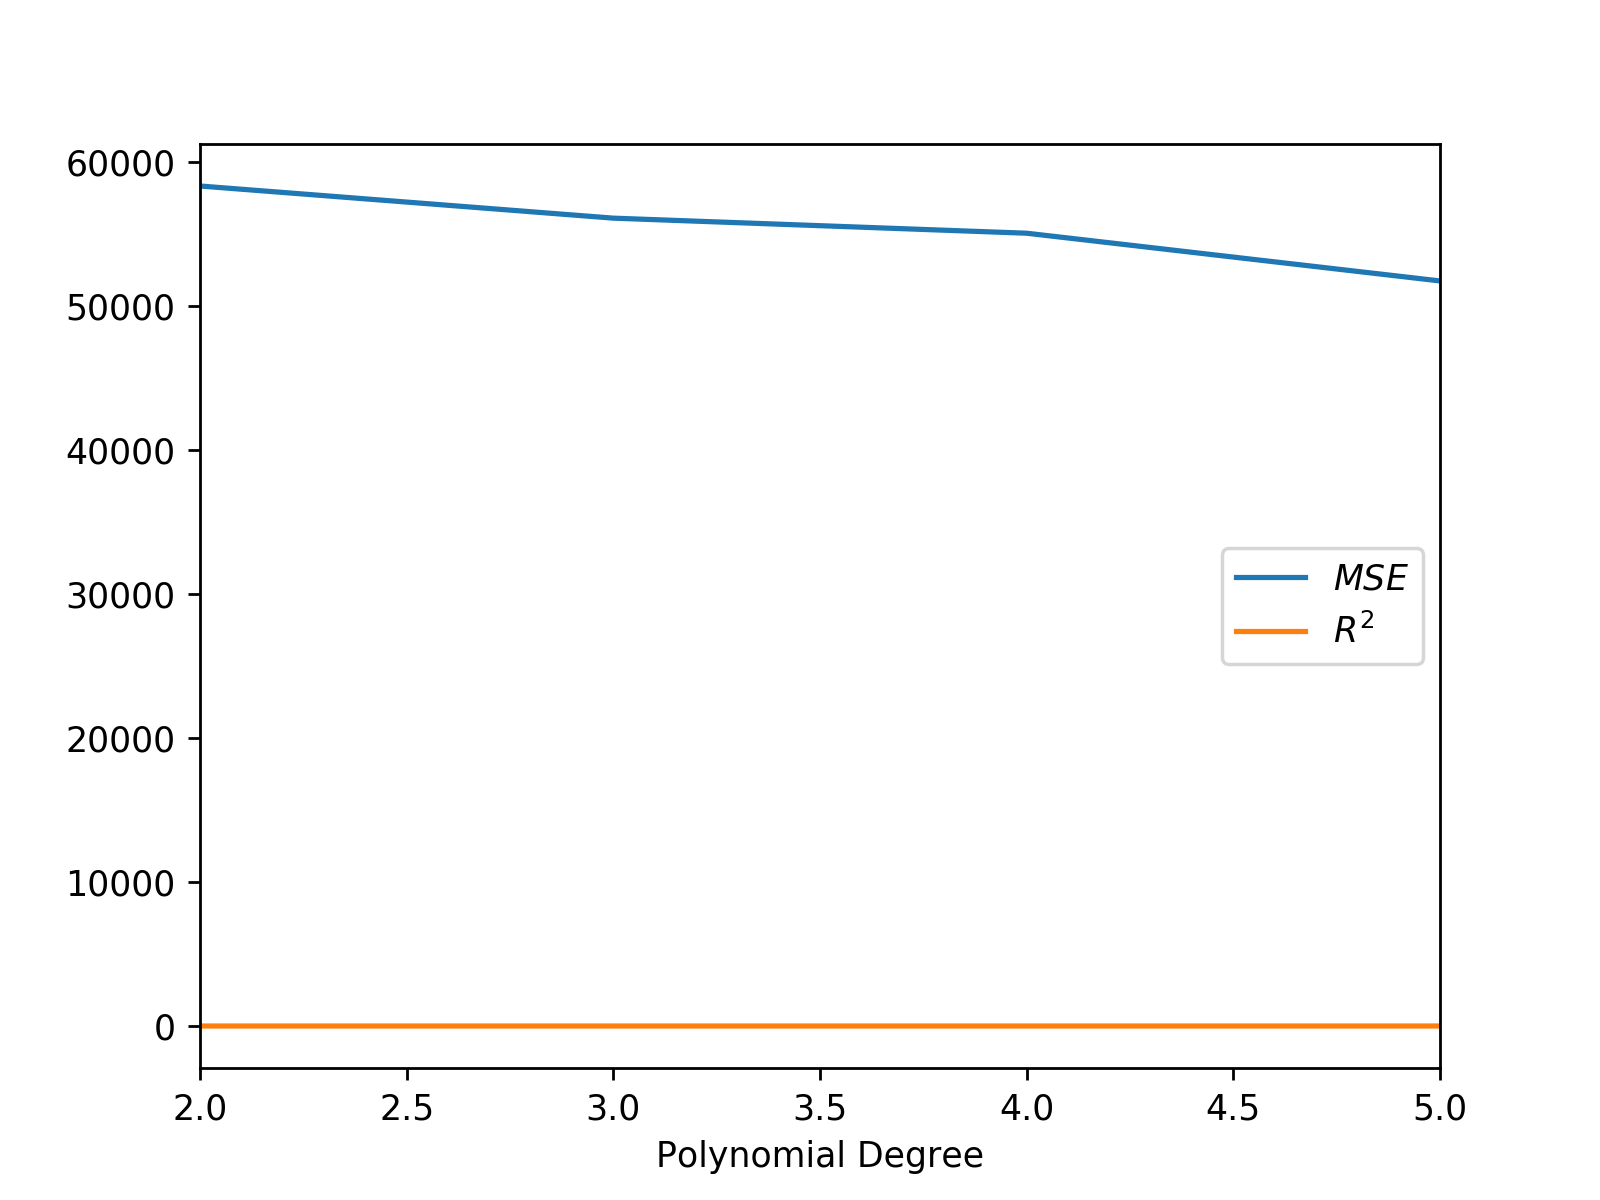
\includegraphics[width = 0.5\textwidth, center]{../real_output/part_B.png}
	\caption{The $MSE$, $R^2$-score and variance $\sigma$ of the vector of coefficients $\beta$ as a function of the polynomial degree after performing \textit{OLS} on real terrain data from \textit{Møsvatn Austfjell}. Using 12-fold cross validation.}
	\label{fig_17}
\end{figure}

\begin{figure}[H]
	\centering 
	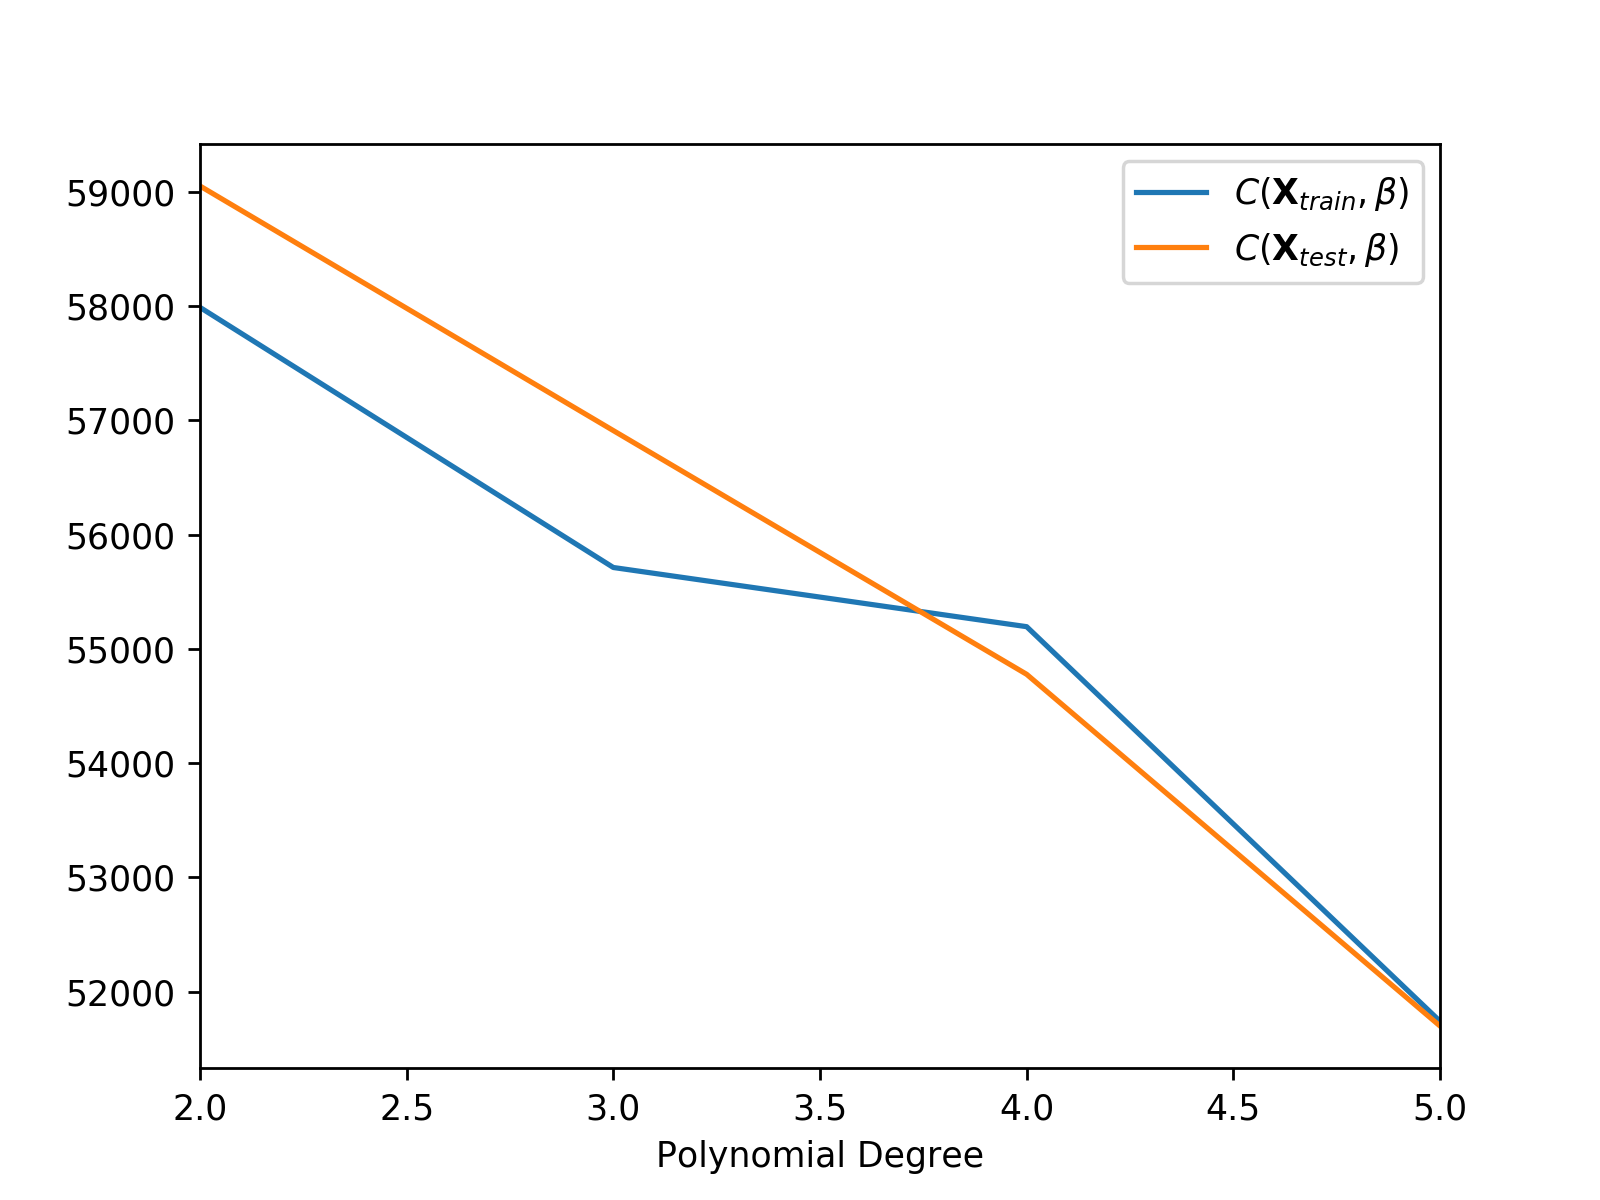
\includegraphics[width = 0.5\textwidth, center]{../real_output/part_C_2.png}
	\caption{The $MSE$ for the \textit{training data} and the \textit{testing data}, as a function of the polynomial degree after performing \textit{OLS} on real terrain data from \textit{Møsvatn Austfjell}}
	\label{fig_18}
\end{figure}

\begin{figure}[H]
	\centering 
	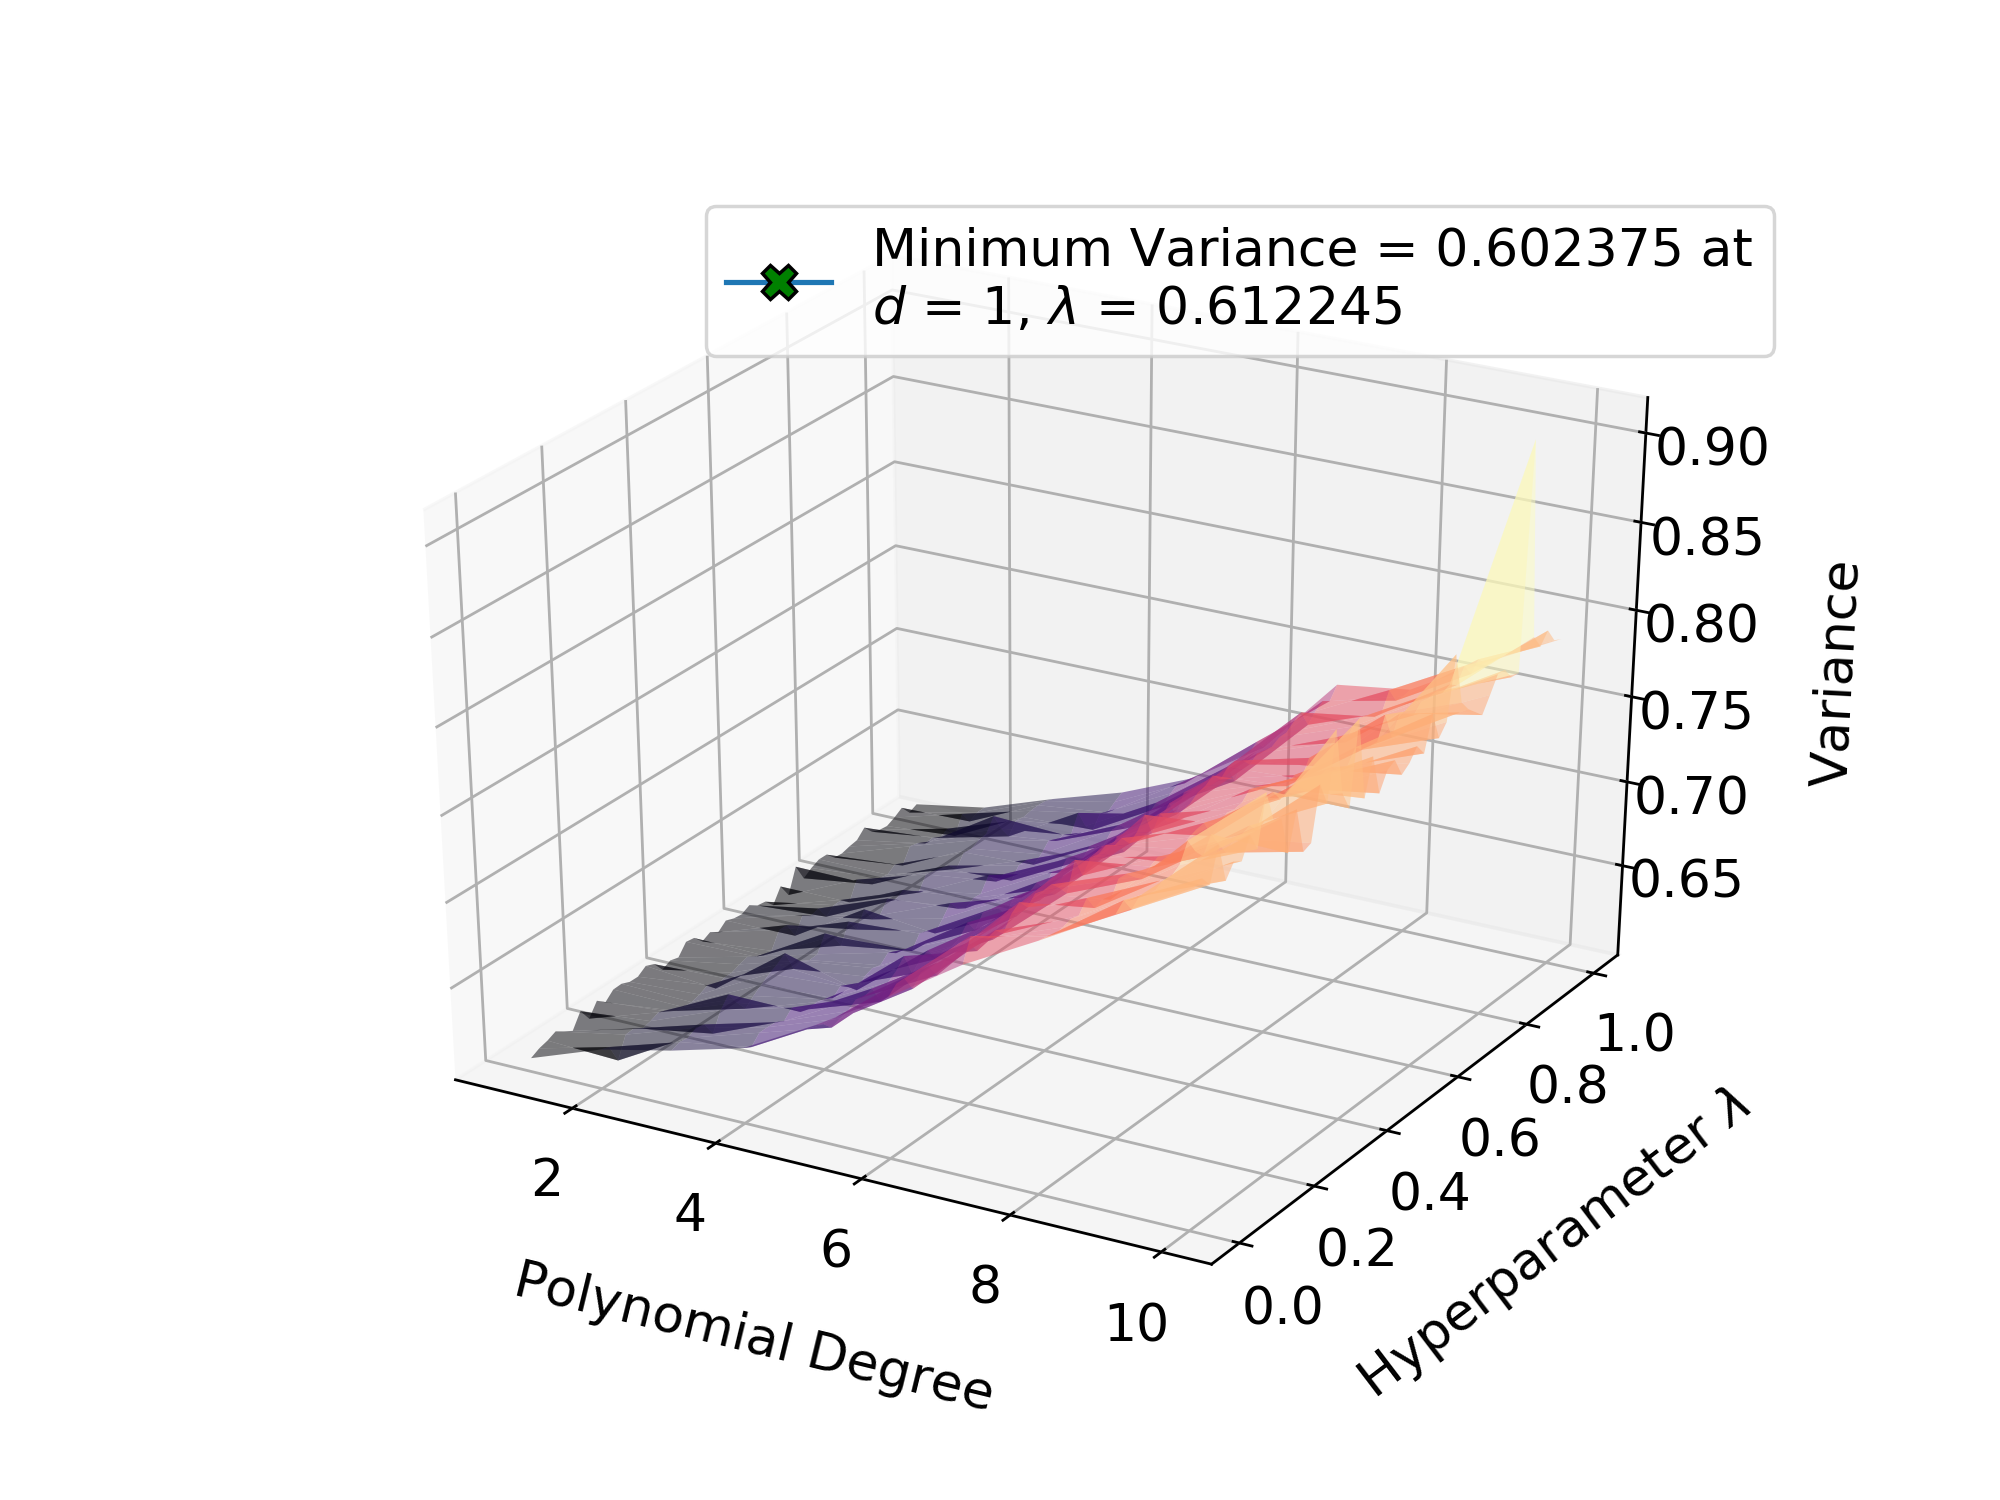
\includegraphics[width = 0.5\textwidth, center]{../real_output/part_D_1.png}
	\caption{The \textit{variance} as a function of the polynomial degree and hyperparameter $\lambda$ after performing \textit{Ridge regression} on real terrain data from \textit{Møsvatn Austfjell}}
	\label{fig_19}
\end{figure}

\begin{figure}[H]
	\centering 
	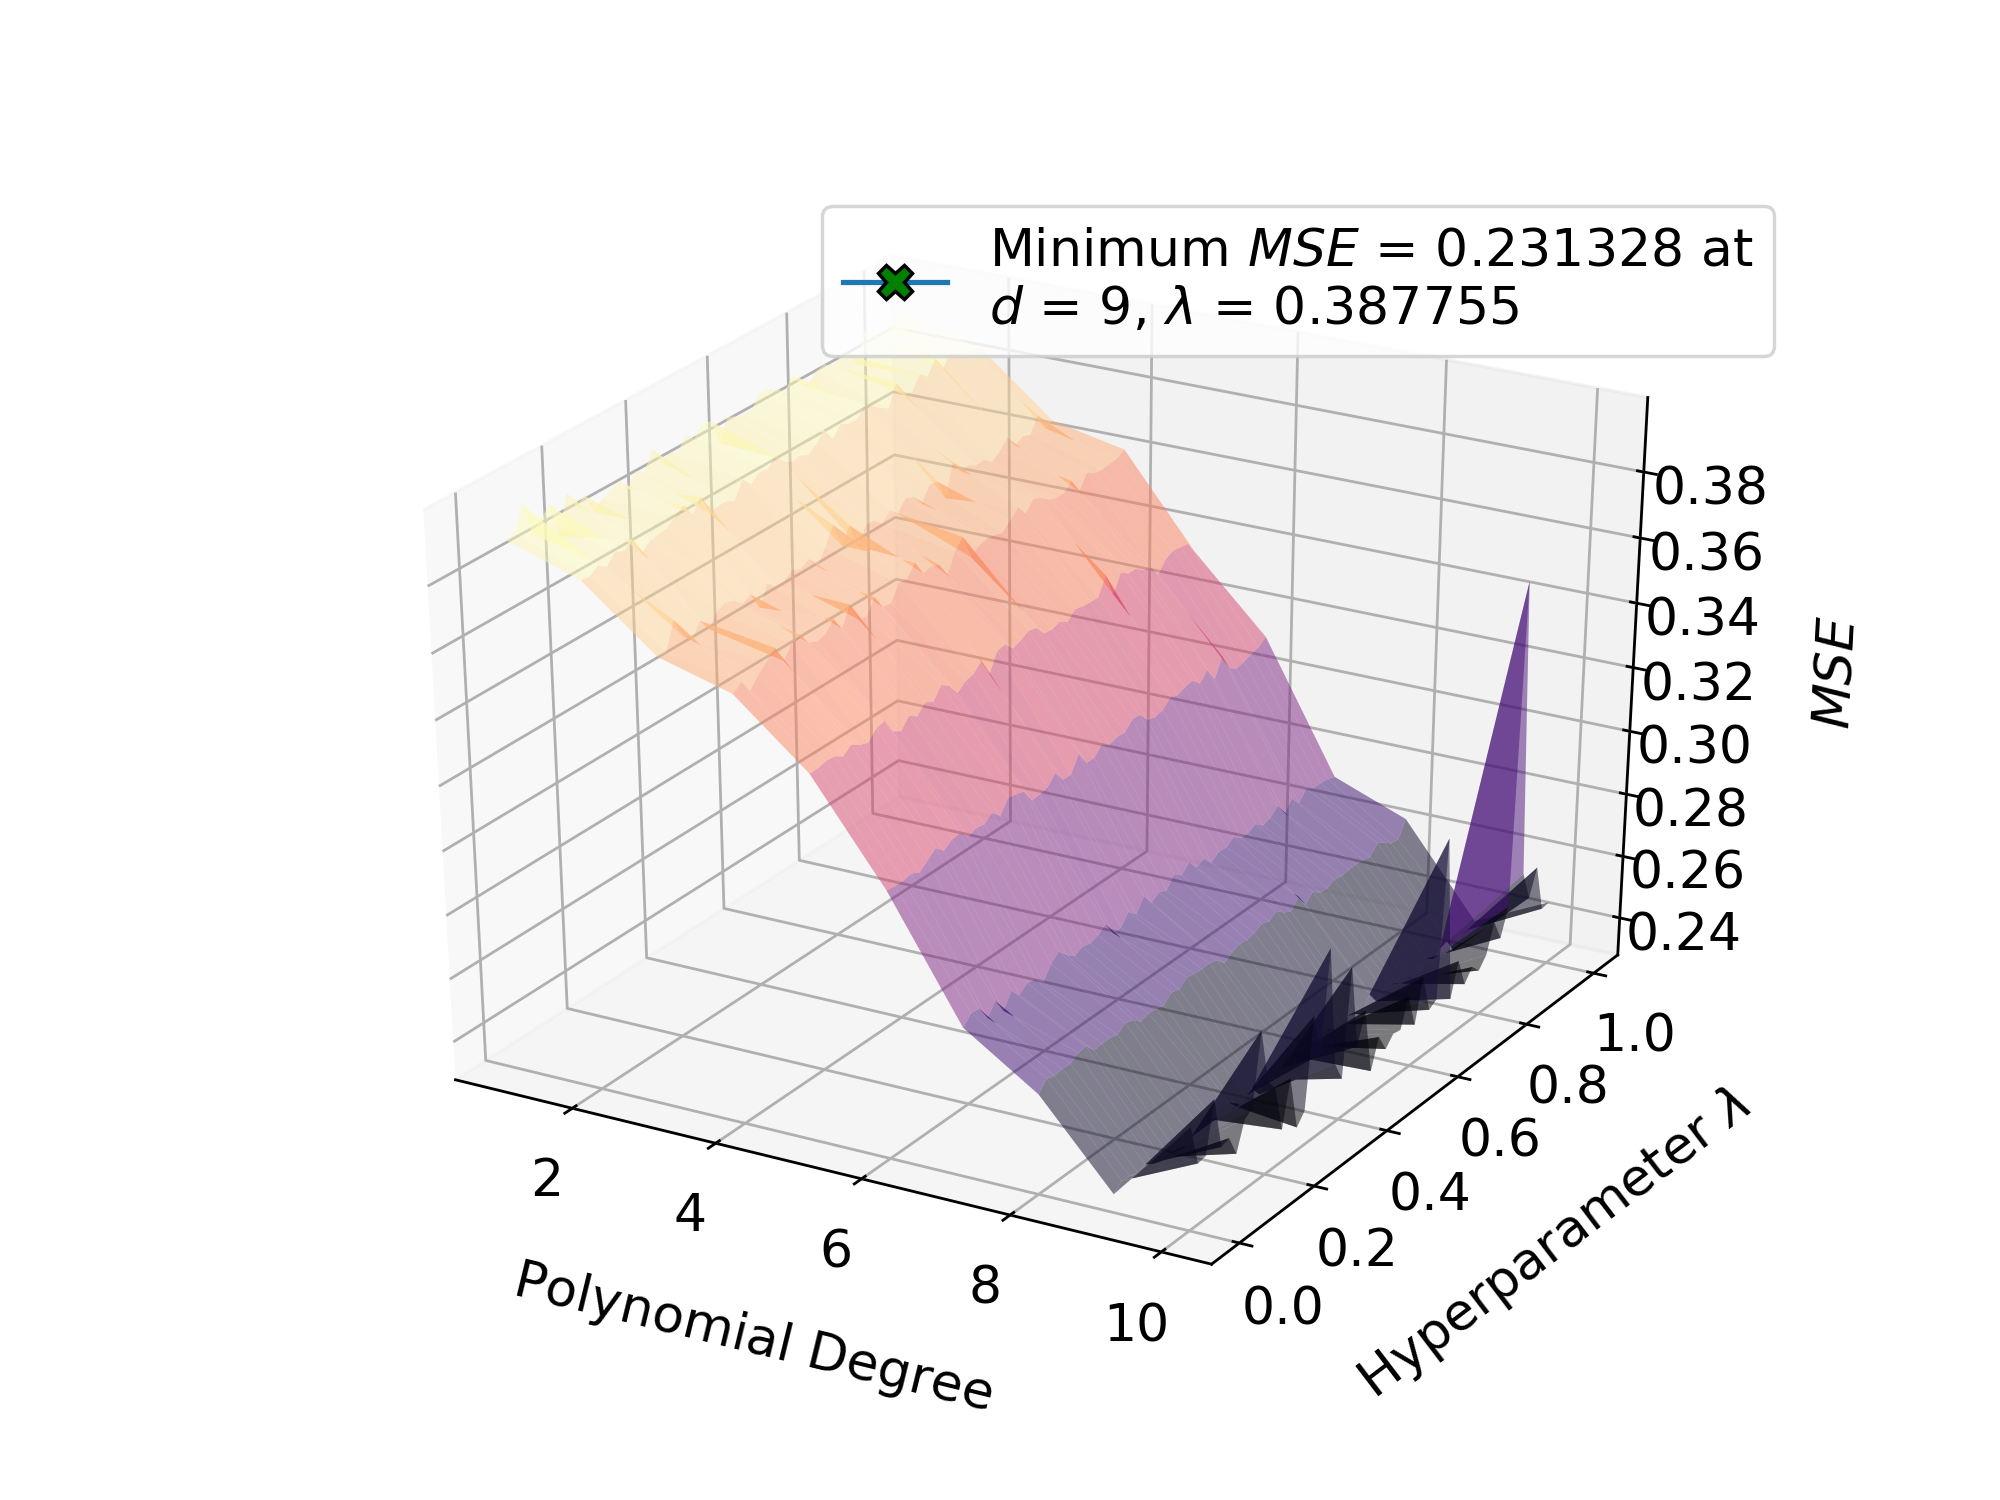
\includegraphics[width = 0.5\textwidth, center]{../real_output/part_D_2.png}
	\caption{The $MSE$ as a function of the polynomial degree and the hyperparameter $\lambda$ after performing \textit{Ridge regression} on real terrain data from \textit{Møsvatn Austfjell}}
	\label{fig_20}
\end{figure}

\begin{figure}[H]
	\centering 
	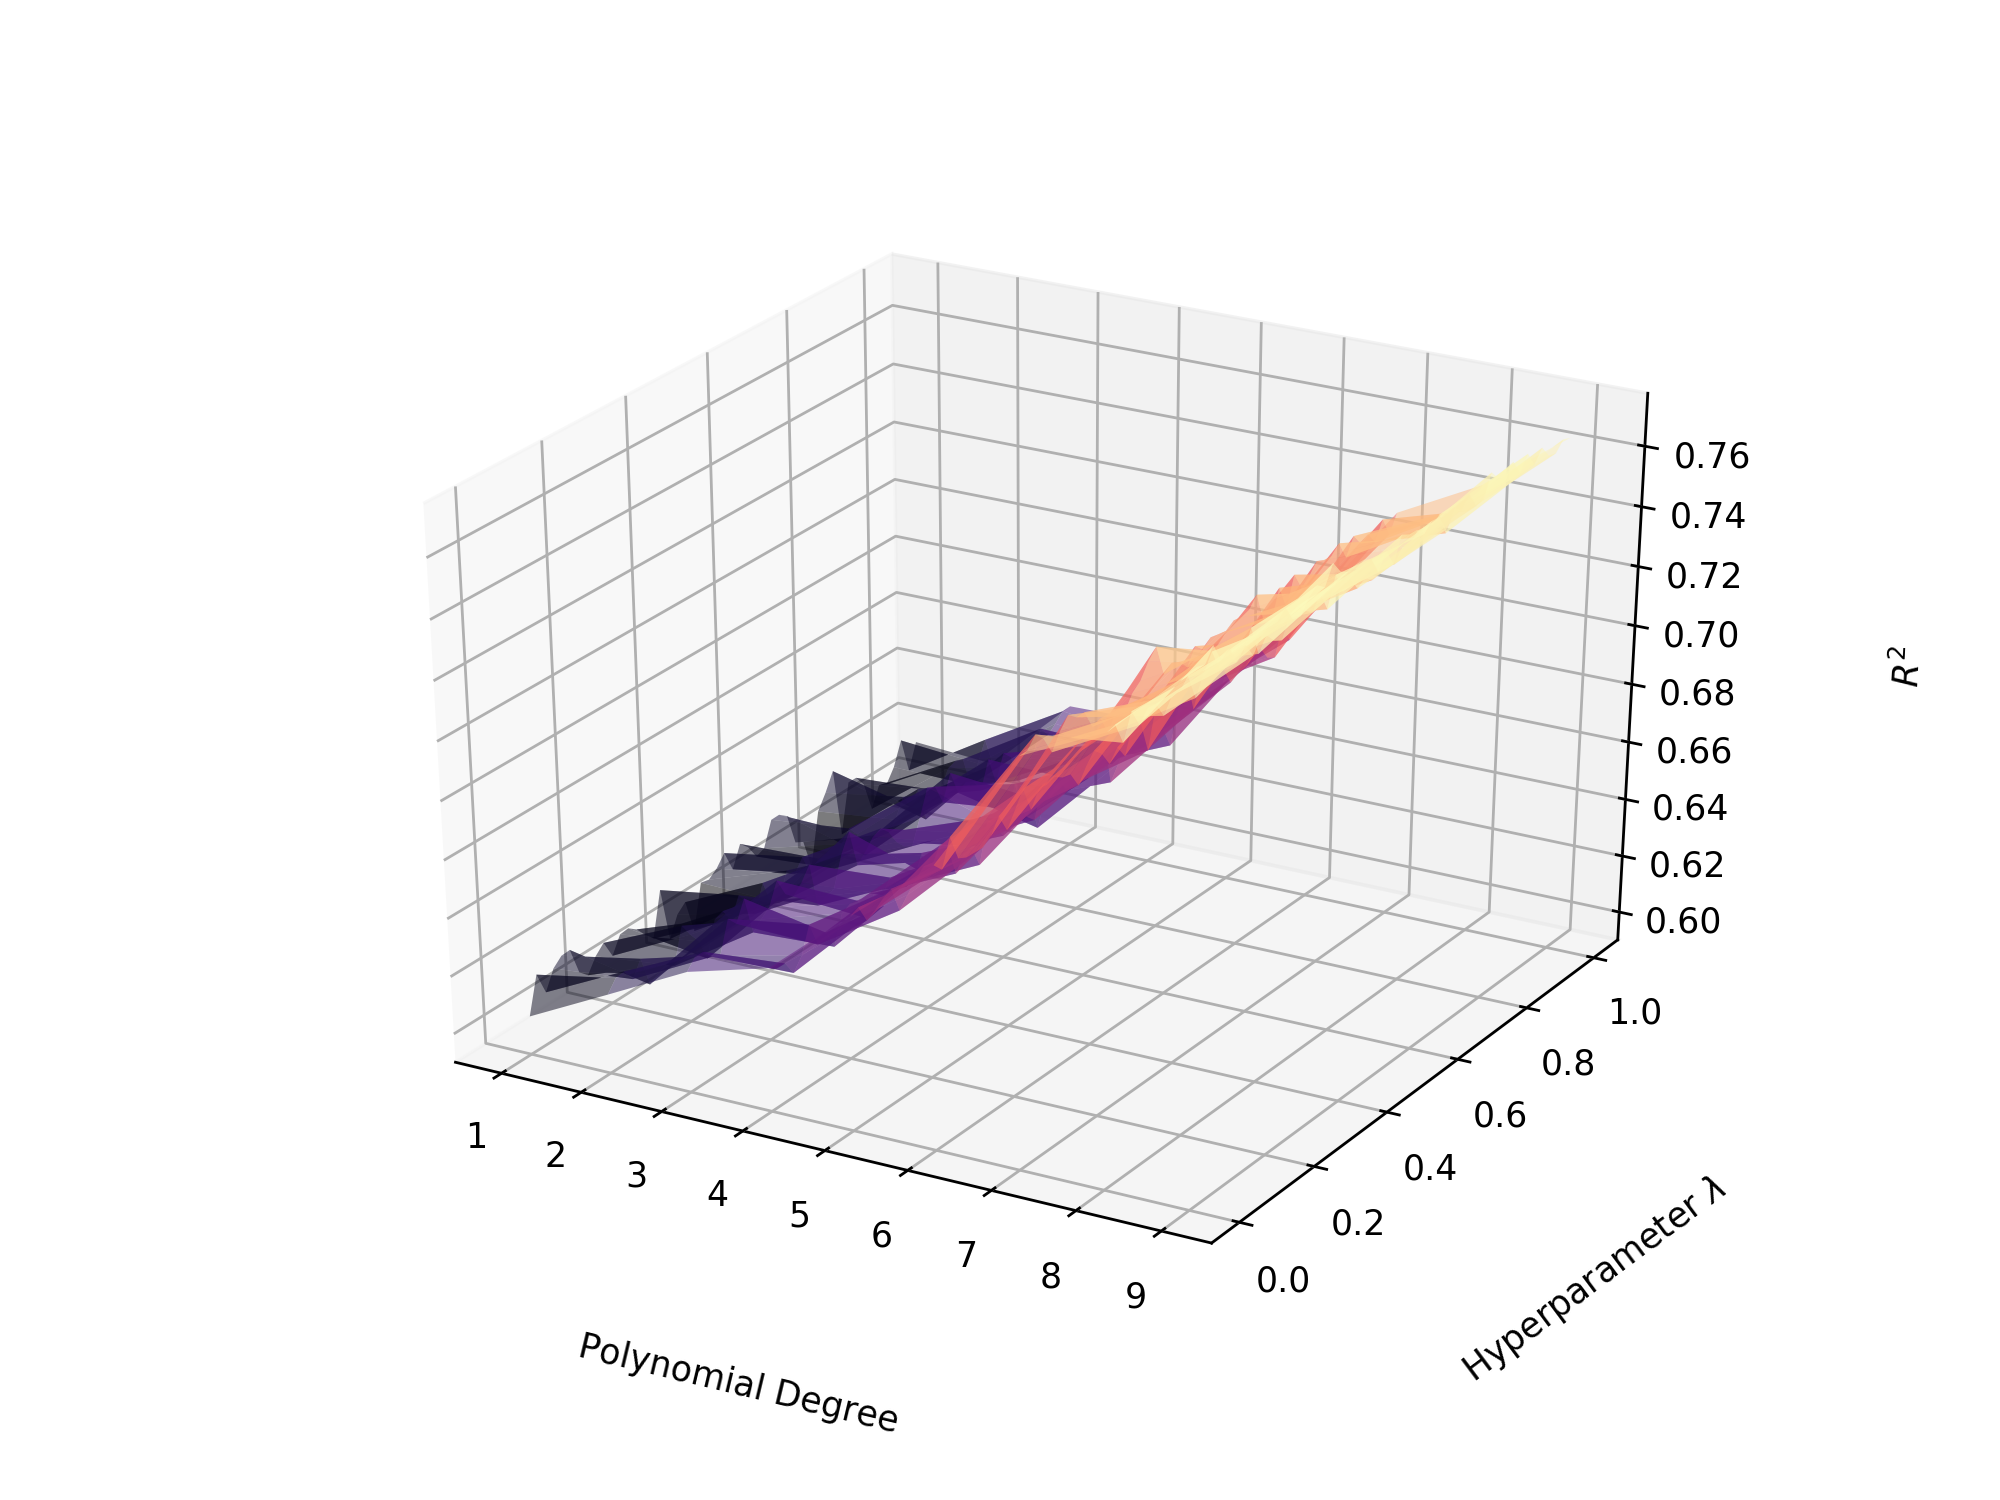
\includegraphics[width = 0.5\textwidth, center]{../real_output/part_D_3.png}
	\caption{The $R^2$-score as a function of the polynomial degree and hyperparameter $\lambda$ after performing \textit{Ridge regression} on real terrain data from \textit{Møsvatn Austfjell}}
	\label{fig_21}
\end{figure}

\begin{figure}[H]
	\centering 
	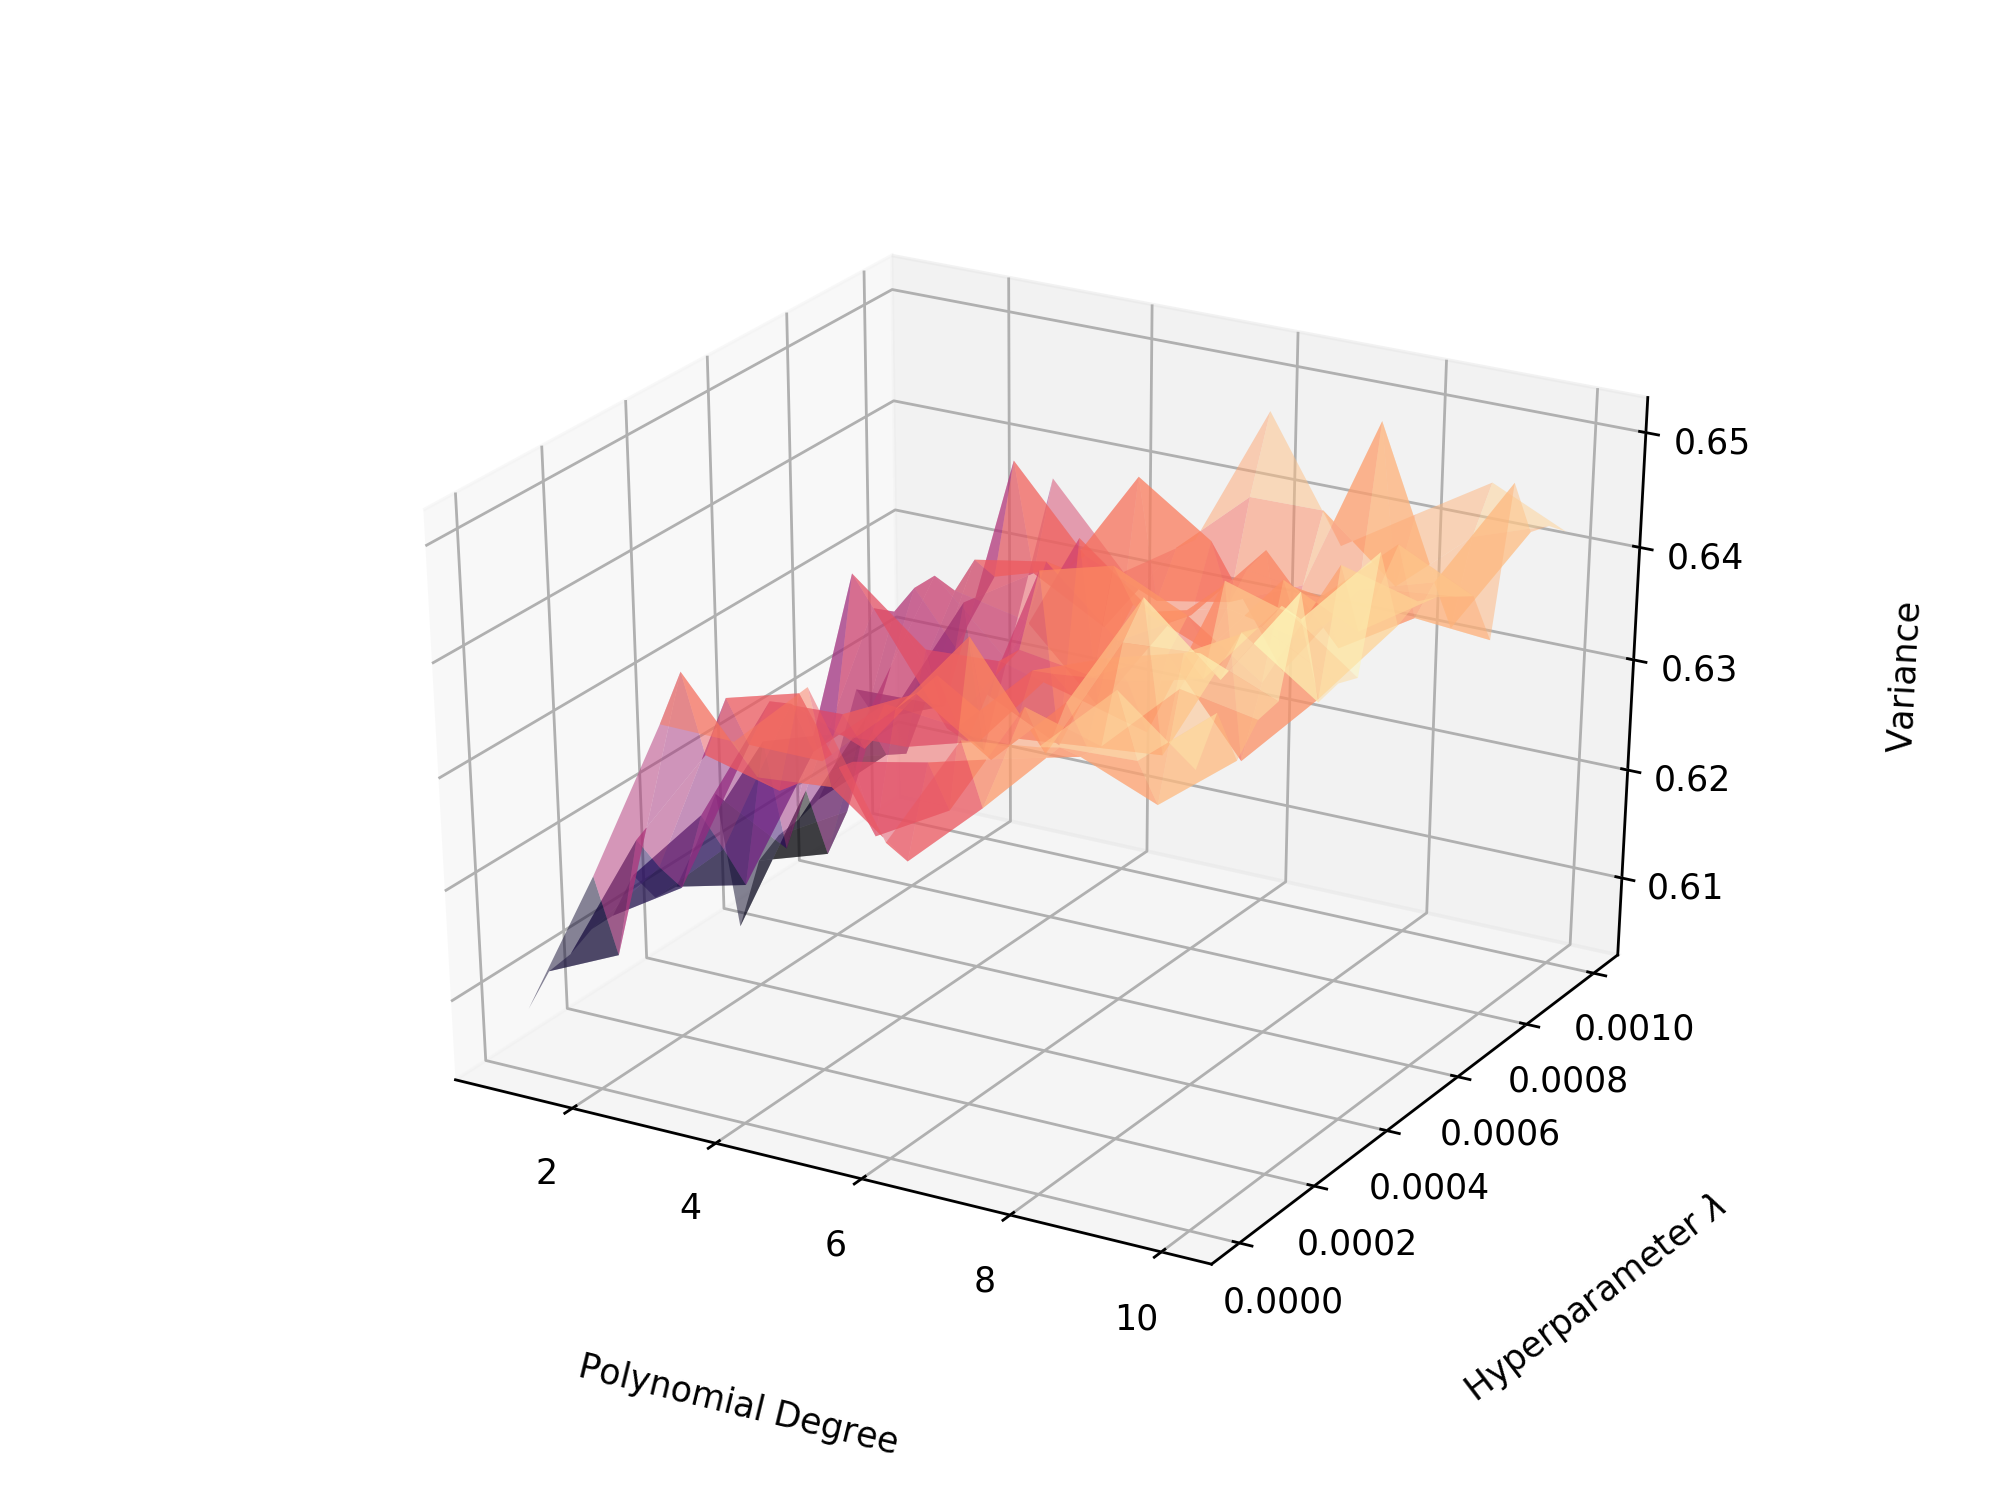
\includegraphics[width = 0.5\textwidth, center]{../real_output/part_E_1.png}
	\caption{The \textit{variance} as a function of the polynomial degree and hyperparameter $\lambda$ after performing \textit{\textsc{lasso} regression} on real terrain data from \textit{Møsvatn Austfjell}}
	\label{fig_22}
\end{figure}

\begin{figure}[H]
	\centering 
	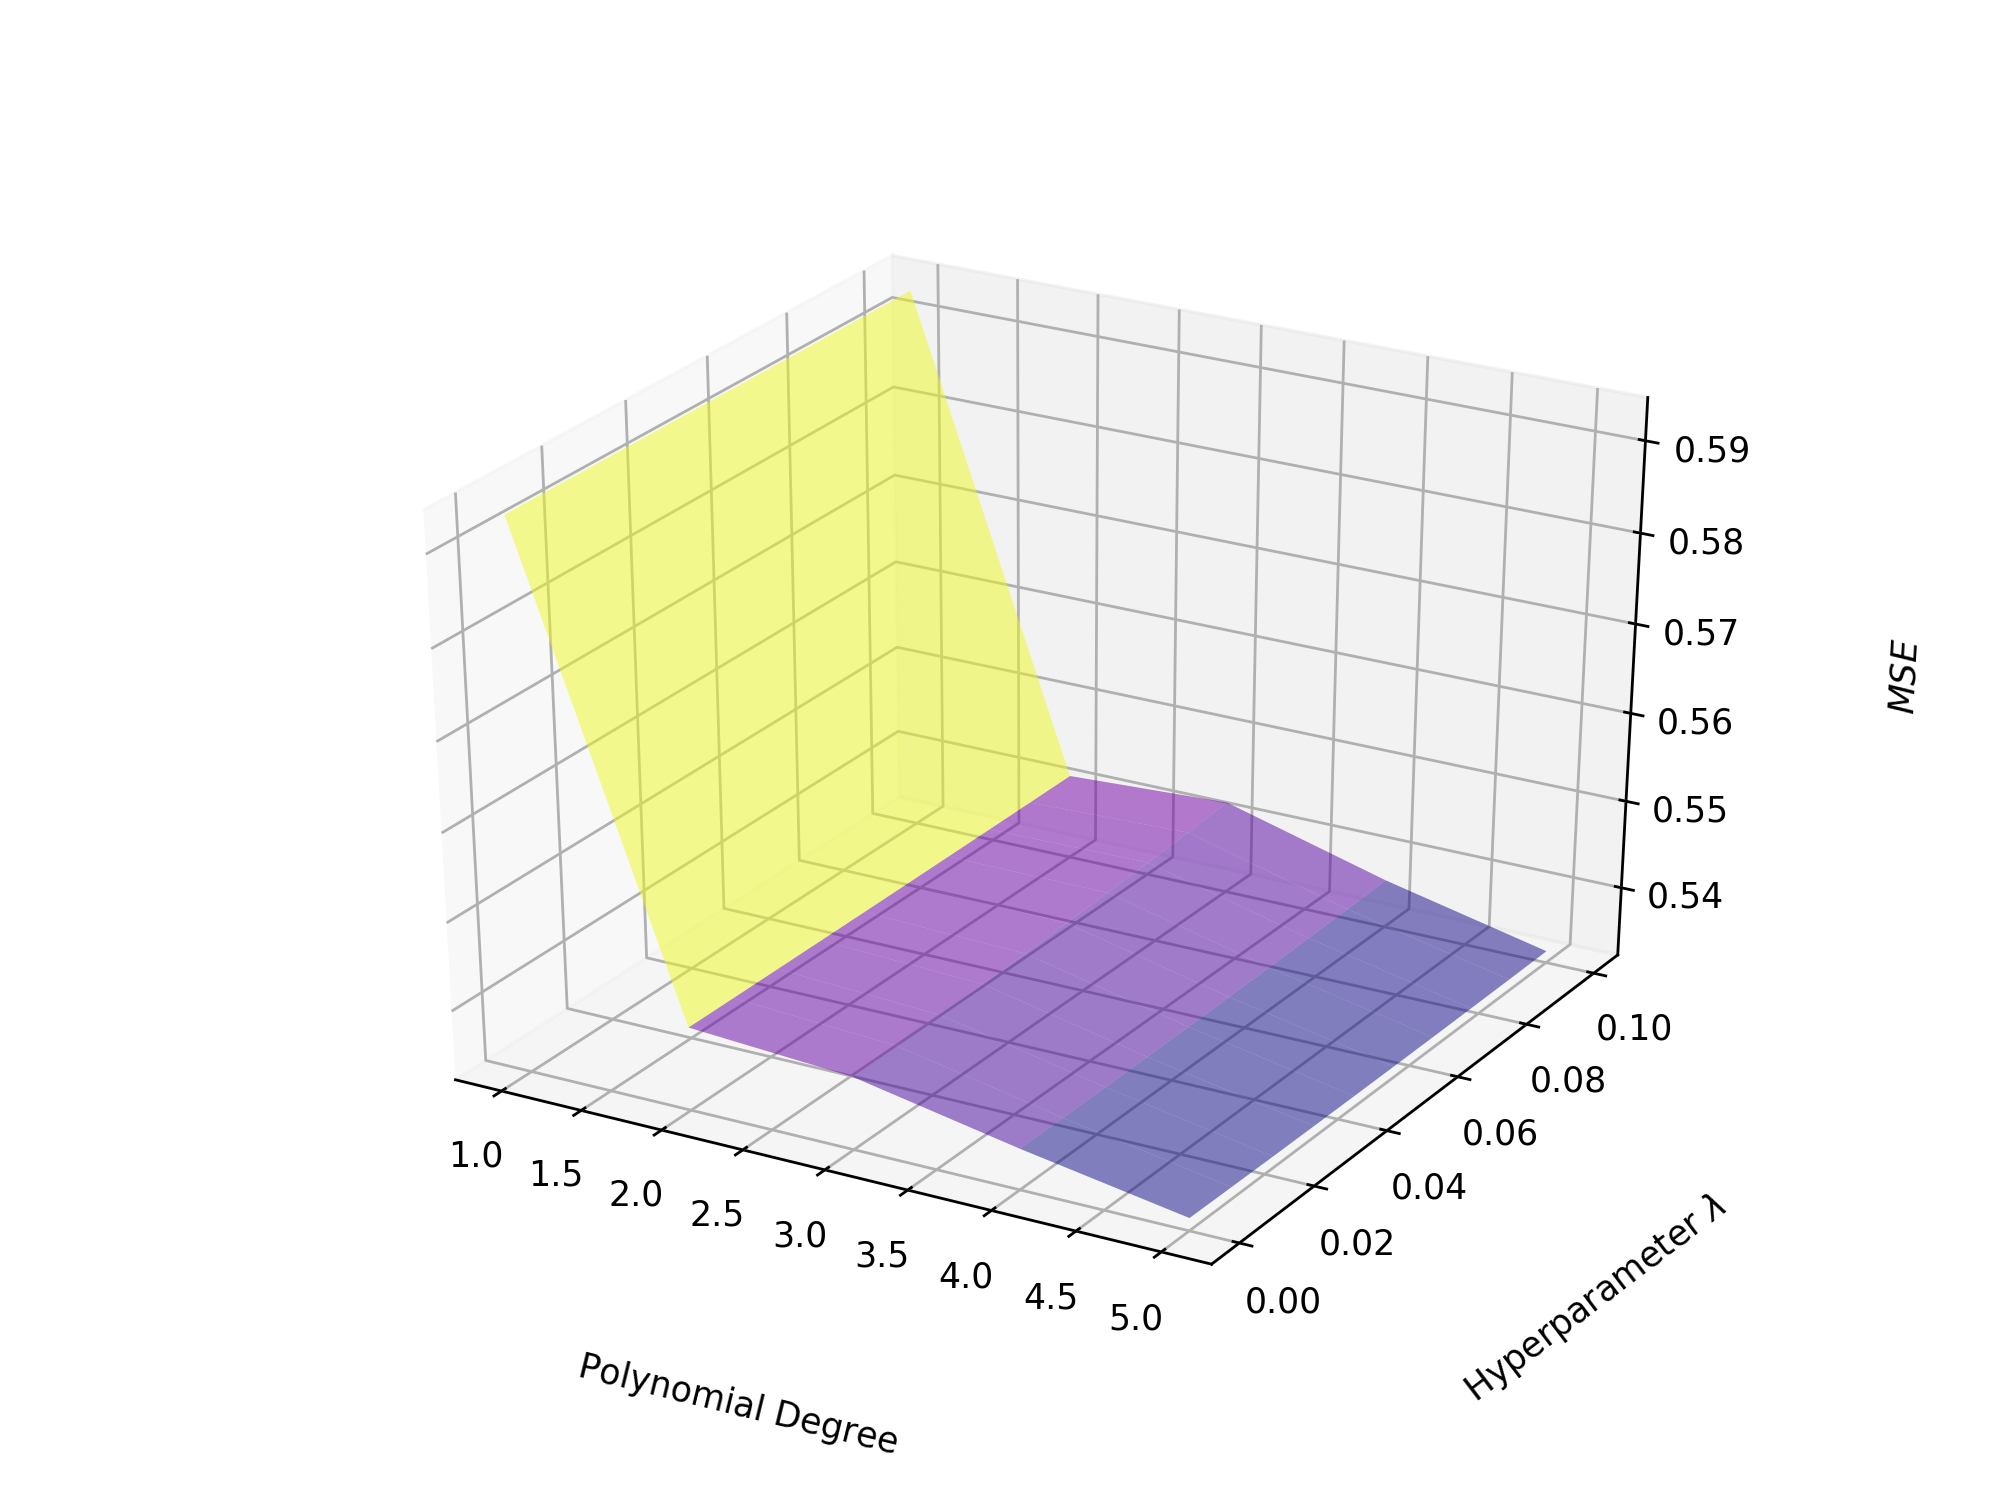
\includegraphics[width = 0.5\textwidth, center]{../real_output/part_E_2.png}
	\caption{Plots of the $MSE$ as a function of the polynomial degree and hyperparameter $\lambda$ after performing \textit{\textsc{lasso} regression} on real terrain data from \textit{Møsvatn Austfjell}}
	\label{fig_23}
\end{figure}

\begin{figure}[H]
	\centering 
	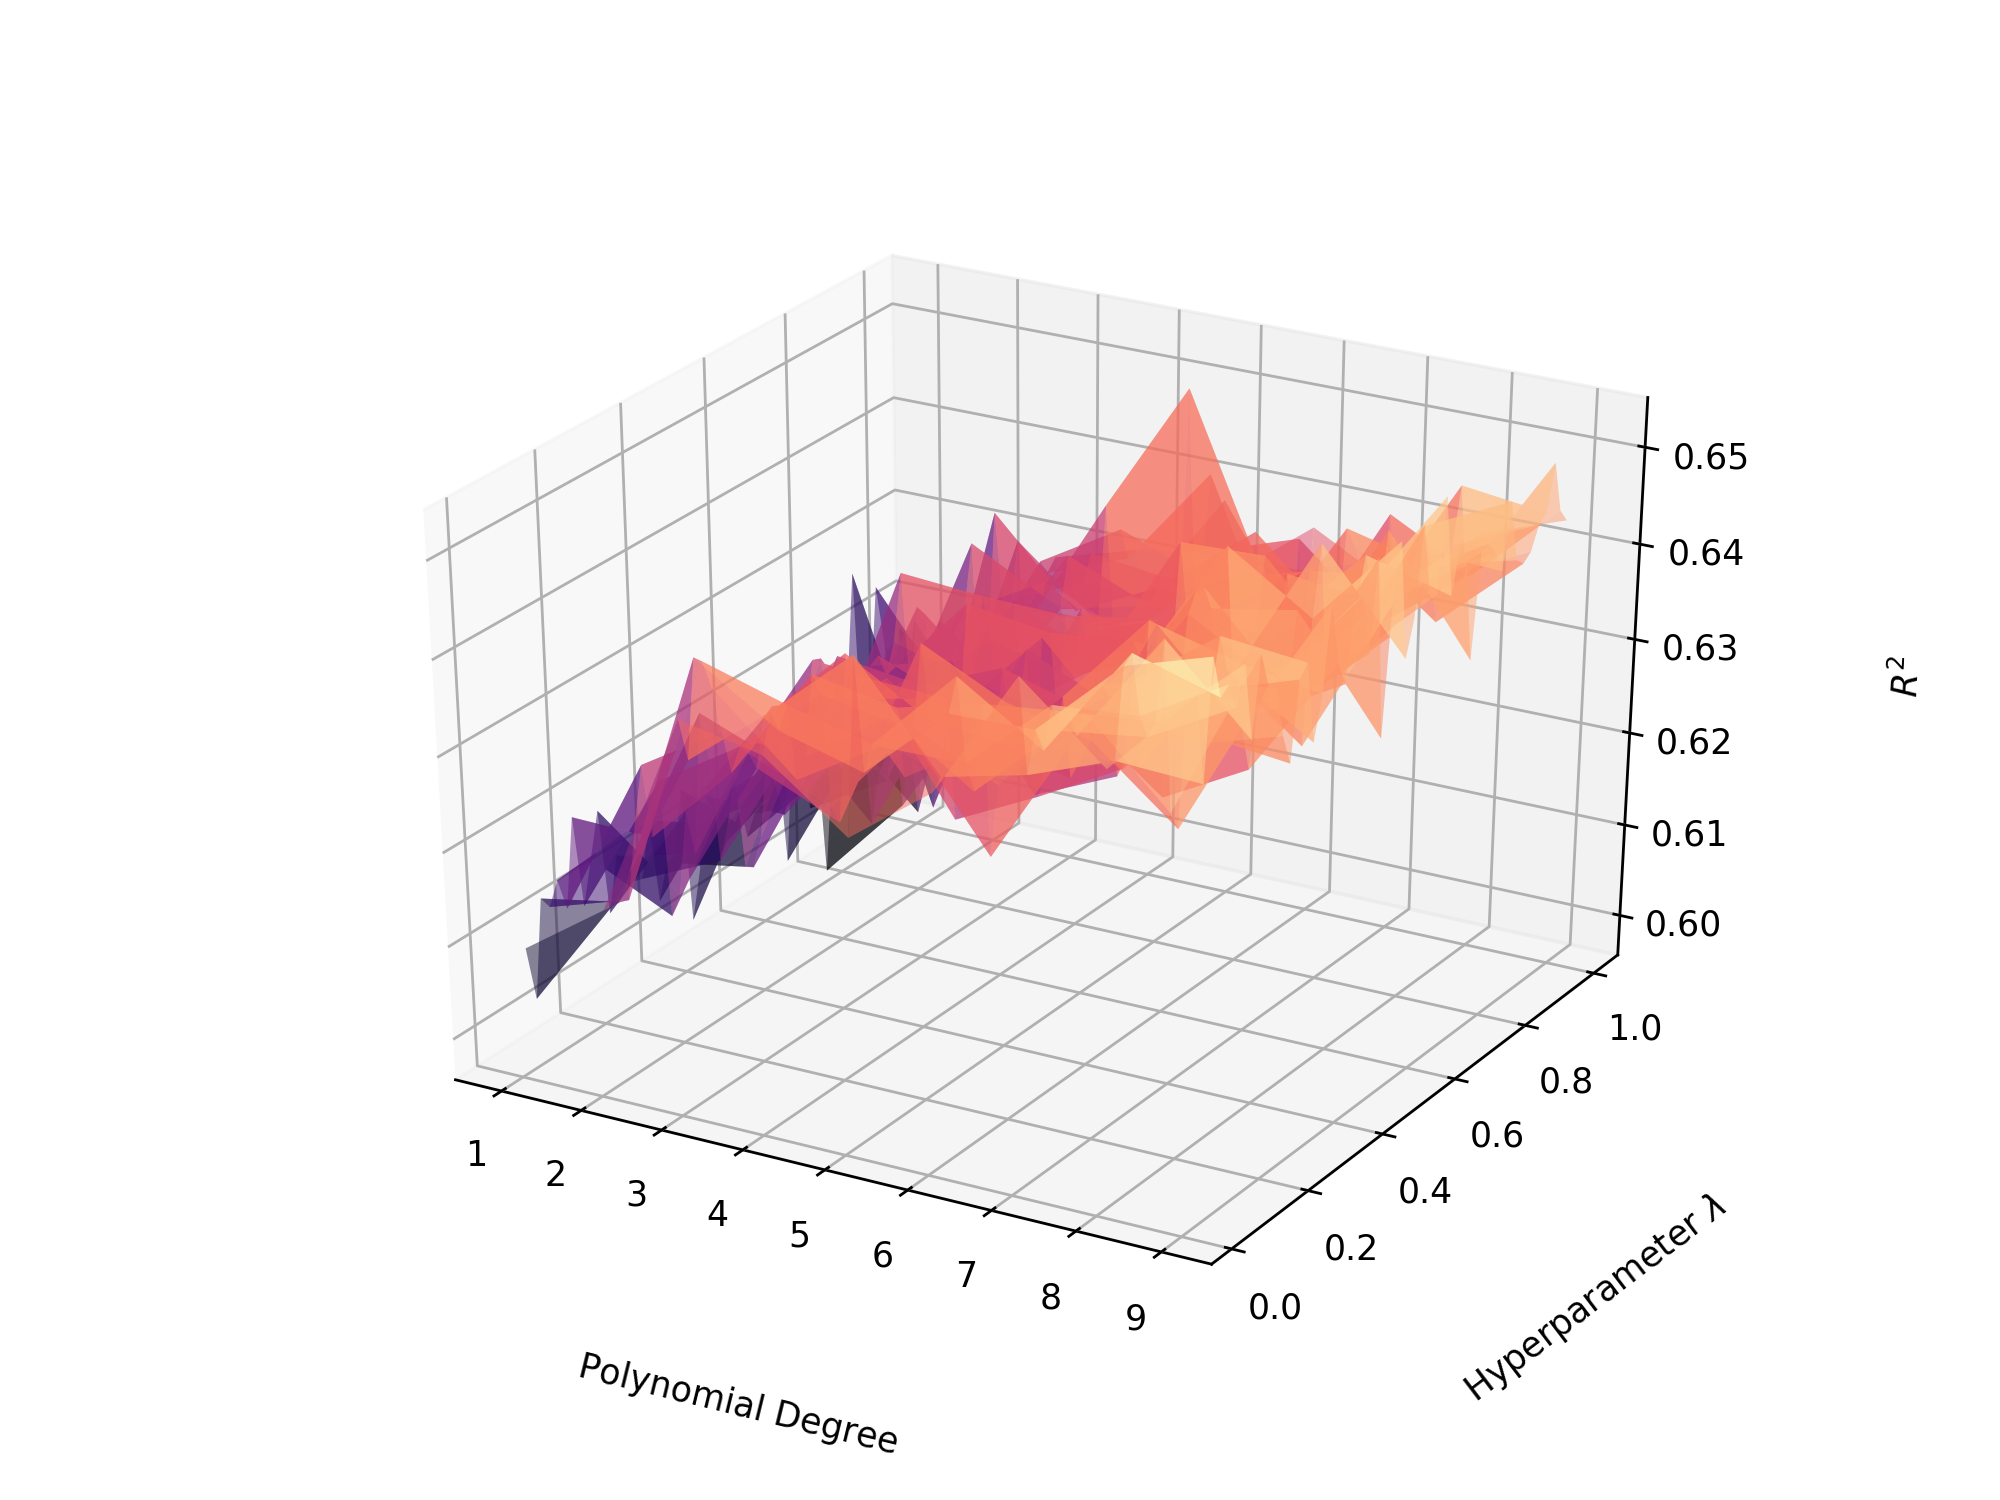
\includegraphics[width = 0.5\textwidth, center]{../real_output/part_E_3.png}
	\caption{The $R^2$-score as a function of the polynomial degre and hyperparameter $\lambda$ after performing \textit{\textsc{lasso} regression} on real terrain data from \textit{Møsvatn Austfjell}}
	\label{fig_24}
\end{figure}

\section*{Discussion}
\label{sec:discussion}

\subsection*{The Franke Function}

In Figure \ref{fig_4}, we see that the \textit{variance} increases as a function of complexity (as expected). It seems that the $R^2$-score also increases up until the polynomial degree reaches 10, where it begins to decrease.  Finally, we see that the $MSE$ decreases, though we will see this more clearly in Figure \ref{fig_7}.
 
In Figure \ref{fig_5}, it appears that implementing cross-validation leaves our results mostly unchanged from those in Figure \ref{fig_4}, though the decrease in the $R^2$-score is somewhat less pronounced.

Given that we know the \textit{Franke function}, we are able to calculate the \textit{bias} (with 12-fold cross-validation) in our model.  In Figure \ref{fig_6} We can see the \textit{bias-variance} tradeoff in action.  

In Figure \ref{fig_7}, we see that the $MSE$, on average, decreases up until we perform a 9\textsuperscript{th}-degree polynomial regression with 12-fold cross-validation\footnote{It can be assumed henceforth that all our data is obtained via 12-fold cross-validation, unless stated otherwise.}, and that this holds for both the \textit{training set} and the \textit{testing set}.

Once we begin to implement \textit{Ridge regression} for hyperparameters $\lambda \in [10^{-12}, 10^{-3}]$, we see that the variance in Figure \ref{fig_8} tends to increase at the same rate for most $\lambda$, with all diverging at degree 10.

In Figure \ref{fig_9}, we see that the $MSE$ decreases as a function of the polynomial degree up until it reaches 10, where it diverges at varying rates over $\lambda$.  In addition to this, we see that the best model for our system may be a 9\textsuperscript{th}-degree polynomial Ridge regression with $\lambda = 10^{-16}$; our $MSE$ is minimized at that point with a value of $2 \times 10^{-4}$.

The maximum $R^2$-score shown in Figure \ref{fig_10} also occurs at $d = 9$ with $\lambda = 10^{-16}$, which further confirm our previous assertions.

The plot of the squared bias in Figure \ref{fig_11}, is essentially a flat plane with a value close to 0.0824.  

Our \textsc{lasso} results are somewhat different.  Here, we see that the variance in Figure \ref{fig_12} depends much more on $\lambda$ than it does in Figure \ref{fig_8}.

The $MSE$ for \textsc{lasso} also differs from that of Ridge regression – in Figure \ref{fig_13}, we see that the optimal polynomial degree is 10, while the ideal $\lambda$ is still $10^{-16}$.
However, this time the $MSE$ is much larger: $0.005$, nearly 20 times that found in Figure \ref{fig_9}.

We see that the $R^2$-score in Figure \ref{fig_14} also performs worse than that in Figure \ref{fig_10}, with an optimal value of 0.94, whereas we have an optimal value of 0.99 in Figure \ref{fig_10}.  However, the ideal polynomial degree per $R^2$ is 9, rather than 10.

The bias for \textsc{lasso} in Figure \ref{fig_15} behaves similarly to that of Ridge regression; as such it is not very important in our evaluation of methods.

\subsection*{Møsvatn Austfjell}

In Figure \ref{fig_16}, we see that the $MSE$, $R^2$-score, and variance each diverge when evaluated for a 10\textsuperscript{th}-degree polynomial regression.

12-fold cross-validation gives us a clearer picture of what is happening, as seen in Figure \ref{fig_17}, where our variance, $MSE$, and $R^2$-score are much more modest than those we saw for the Franke function.

A closer look at the $MSE$ (of both the \textit{training set} and the \textit{testing set}) in Figure \ref{fig_18} show that a polynomial of degree 9 is optimal when performing OLS.

Figure \ref{fig_19}, which shows the variance as a function of polynomial degree and hyperparameter $\lambda$, behaves differently than it's Franke function counterpart\footnote{Seen in Figure \ref{fig_8}}; instead of flattening out, the variance consistently grows as the polynomial degree is increased\footnote{Though it is mostly constant with respect to $\lambda$.}

Interestingly enough, we see that the optimal polynomial degree in Figure \ref{fig_20} is 9, just as for the Franke function \footnote{Seen in Figure \ref{fig_9}.}.  However, the minimum $MSE$ is much larger than that of the Franke function, at 0.23, and the optimal hyperparameter is now $\lambda = 0.655$.

Figure \ref{fig_21} suggests a different hyperparameter of $\lambda = 0.31$, but continues to select 9 as the optimal polynomial degree.

Our implementation of \textsc{lasso} yields very different results now when dealing with this real life data.  We see in Figure \ref{fig_22} that there is much less stability in this variance, than that of the corresponding Figure \ref{fig_19}.

As for the optimal $MSE$ of our \textsc{lasso} regression, we see in Figure \ref{fig_23} that a polynomial of 10\textsuperscript{th} degree is optimal, with a minimum $MSE$ of 0.348. 

Finally, we see that our $R^2$-score in Figure \ref{fig_24} has an optimal value of 0.651, while still suggesting that a polynomial of degree 10 would give us the best results.

\section*{Conclusion}

This is likely due to the fact that we implemented matrix inversion without implementing the SVD. Perhaps a more robust algorithm would lead to higher degree polynomials giving us better values in the MSE, but the variance would certainly continue to increase. 

K-fold cross-validation is known to produce more stable results, as we discussed in our method section.

Interestingly enough, it seems as though our bias does not decrease as much as expected. 

We assume the reason that the $MSE$ begins to diverge once we perform a 10\textsuperscript{th}-degree polynomial regression is due to floating-point errors.

It is likely numerical instability that leads to diverging at varying rates, and this can likely not be avoided, though implementing the SVD might help.

It also seems that the our $MSE$ increases as a function of the hyperparameter $\lambda$, and that $10^{-16}$ is our best choice since smaller values will lead to floating point errors.

Given that the $R^2$-score in Figure \ref{fig_10} agrees as well, this could very well be the case.

We can assume that the variation in Figure \ref{fig_11} is simply a product of random number generation.

Perhaps if we had greater numerical precision, such as 128-bit precision, then we might be able to further decrease $\lambda$ and get even better results.

It is very likely that allowing the \textsc{lasso} function to converge at a larger number of iterations would improve the $MSE$.

Given the inconsistencies in \textsc{lasso}, as well as the fact that it performs worse on both the $MSE$ and $R^2$, it seems apparent that Ridge regression with an optimized $\lambda$ may be our ideal model.

It appears that cross-validation is necessary when dealing with a real life dataset, especially if given a dataset that is particularly sparse.

Once again, the fact that we are dealing with real life data leads to worse performance with regards to the $MSE$ and other validation metrics.

With a minimum $MSE$ of 0.25, we have to accept a good deal of imprecision in our regression, but that is simply a consequence of dealing with real data.  However, we can be confident that our model performs reliably, as the $MSE$ curves for the training and testing sets in Figure \ref{fig_18} differ little.

Since the geological features of our dataset do not match any polynomial particularly well, increasing the polynomial degree in Ridge regression will always lead to a larger variance.

The fact that two vastly different datasets \footnote{One a mathematical function, the other a scan of a landscape.} both have optimal polynomial regression degrees of 9, is suspicious.  We suspect that implementing another method, such as the SVD, might lead to more stability in our model; if this is to be the case, perhaps a higher degree polynomial regression would be successful, and reduce the $MSE$ further.

Perhaps the most important conclusion we can draw from our experience here is that when dealing with real life data, implementing Ridge regression over OLS is likely unnecessary, as we see that our results are all mostly independent of the hyperparameter $\lambda$.

It is also worth mentioning that \textsc{lasso} performs with far less stability than OLS or Ridge regression, and with a noticeably larger $MSE$ and variance, and smaller $R^2$-score.  It is likely that increasing the iteration limit for \textsc{lasso} would help improve this, but at an extreme performance penalty.

We should also note that the $MSE$, variance, and $R^2$ are all likely independent of the chosen hyperparameter $\lambda$ for \textsc{lasso}, just as they were for Ridge regression.

If we can draw any conclusion, it is that OLS and Ridge regression are equals when it comes to their performance, and that \textsc{lasso} gives poorer results.  This may not be the case if we allow for the \textsc{lasso} algorithm to iterate a larger number of times, but this is simply not possible given the constraints of our equipment.

\bibliography{bib}{}
\bibliographystyle{ieeetr}

\end{document}